% concatenated from main.tex
\documentclass[11pt,a4paper]{article}

\usepackage[utf8]{inputenc}
\usepackage[T1]{fontenc}
%\usepackage{geometry}
%\geometry{margin=2.5cm}
\usepackage{flafter,amsmath,amssymb,latexsym,psfrag,graphicx,color,indentfirst,bm}
\usepackage[amsthm]{ntheorem}
\theorembodyfont{\itshape}
\usepackage{mathrsfs}
\usepackage{bm}
\usepackage{enumerate}
\usepackage{hyperref}
\usepackage{xcolor}
\usepackage{float}
\numberwithin{equation}{section}
\newtheorem{theorem}{Theorem}[section]
\newtheorem{proposition}[theorem]{Proposition}
\newtheorem{lemma}[theorem]{Lemma}
\newtheorem{corollary}[theorem]{Corollary}
\newtheorem{assumption}{Assumption}
\newtheorem{property}[theorem]{Property}
\newtheorem{definition}{Definition}
\newtheorem{remark}[theorem]{Remark}
\newtheorem{problem}[theorem]{Problem}
\usepackage[T1]{fontenc}
\usepackage[utf8]{inputenc}
\usepackage{dutchcal}

\usepackage{hyperref}
\hypersetup{
    colorlinks=true,
    linkcolor=blue,
    urlcolor=red
}
\usepackage[a4paper,top=2cm,bottom=2cm,left=2cm,right=2cm, marginparwidth=1.75cm]{geometry}
\usepackage{tikz}
\usetikzlibrary{arrows.meta, shapes.geometric, patterns, calc}
\newcommand{\R}{\mathbb{R}}
\newcommand{\C}{\mathbb{C}}
\newcommand{\N}{\mathbb{N}}
\newcommand{\Z}{\mathbb{Z}}

\newcommand{\Om}{\Omega}
\newcommand{\om}{\omega}
\newcommand{\veps}{\varepsilon}
\newcommand{\eps}{\varepsilon}
\newcommand{\dd}{\,\mathrm{d}}
\usepackage{comment}
\newcommand{\norm}[1]{\left\lVert #1 \right\rVert}
\newcommand{\abs}[1]{\left\lvert #1 \right\rvert}
\newcommand{\ip}[2]{\left\langle #1,#2 \right\rangle}
\usepackage{physics}
\DeclareMathOperator{\Div}{div}
\DeclareMathOperator{\supp}{supp}
\DeclareMathOperator{\dist}{dist}
\DeclareMathOperator{\Id}{Id}
\definecolor{revisionmagenta}{RGB}{180,0,120}
\definecolor{localizationgreen}{RGB}{0,105,80}
\definecolor{rankclarification}{RGB}{0,80,180}
\definecolor{clustercompression}{RGB}{120,35,150}
\newcommand{\rev}[1]{\textcolor{revisionmagenta}{#1}}
\newcommand{\locrev}[1]{{\color{localizationgreen}#1}}
\newcommand{\rankrev}[1]{{\color{rankclarification}#1}}
\newcommand{\clusterrev}[1]{{\color{clustercompression}#1}}


%------------------------------------------
\usepackage{mathrsfs}
\newsavebox\foobox
\newlength{\foodim}
\newcommand{\slantbox}[2][0]{\mbox{%
        \sbox{\foobox}{#2}%
        \foodim=#1\wd\foobox
        \hskip \wd\foobox
        \hskip -0.5\foodim
        \pdfsave
        \pdfsetmatrix{1 0 #1 1}%
        \llap{\usebox{\foobox}}%
        \pdfrestore
        \hskip 0.5\foodim
}}
\def\Laplace{\slantbox[-.45]{$\mathscr{L}$}}
\def\Fourier{\slantbox[-.45]{$\mathscr{F}$}}
\def\bsq#1{%both single quotes
\lq{#1}\rq}
%------------------------------------------

\title{%Pressure Tracking for the Acoustic Wave Equation\\
%via Resonant Bubble Actuators\\
\textbf{Resonant Microstructures as Dirac-type Actuators\\ for Acoustic Wave Control}
%\textbf{Asymptotic Realization of Dirac Actuators for Interior Acoustic Control via High-Contrast Resonant Perturbations}
}
%and some Quantitative Bounds using Harary Graph
\author{Arpan Mukherjee\footnote{MSU-BIT SMBU Joint Research Center of Applied Mathematics, Shenzhen MSU-BIT University, Shenzhen, People's Republic of China (arpan.mukherjee@smbu.edu.cn and arpanmath99@alumni.iitm.ac.in).} \ and
Mourad Sini\thanks{Radon institute, RICAM, Austrian Academy of Sciences, Altenbergerstrasse 69, 4040 Linz, Austria (mourad.sini@oeaw.ac.at). The work of M. Sini is partially supported by the Austrian Science Fund (FWF): P 32660 and  P: 36942.}}

\date{\today}

\begin{document}

\maketitle

\begin{abstract}




\bigskip

We study interior control of the acoustic wave equation via effective point sources generated by a finite cluster of resonant perturbations (modeling acoustic subwavelength bubbles). At the abstract level, after localizing the whole-space dynamics to a large auxiliary observation domain, we consider a Dirichlet spectral formulation of the wave equation with finitely many point actuators located at prescribed interior points. Restricting to a finite spectral band of Dirichlet eigenfrequencies, we prove that, under a natural full-rank condition on the associated coupling matrix, arbitrary trajectories on the corresponding spectral subspace can be realized, with quantitative bounds on the control cost in terms of spectral-band geometry and actuator placement.
\newline
We then show that these ideal actuators can be realized by clusters of small, high-contrast bubbles. Using a time-domain asymptotic expansion, the scattered field is represented as a superposition of retarded monopoles whose amplitudes satisfy a finite-dimensional delayed hyperbolic system. In the Laplace domain, this induces a transfer operator whose pole structure encodes the Minnaert resonance with a collective attenuation.
\newline
We prove that the associated actuator map is ill-conditioned away from resonance, whereas, under a cluster-level transducer accessibility condition linking the incident fields to the dominant cluster channels, it admits a bounded right inverse on suitable Minnaert bands. Consequently, one obtains spectral tracking of the wave field with error $\mathcal{O}(\varepsilon^\gamma)$ as the bubble size $\varepsilon \to 0$.


\medskip
\noindent
\textbf{Keywords.} Wave equation, Dirac actuators, Trajectory tracking control, Resonant perturbations, Kato's analytic perturbation, Perron-Frobenius spectrum, Minnaert resonances, Actuation map, Toeplitz matrix.

\end{abstract}

\tableofcontents

%\section{Introduction: Setting, Mathematical Formulation, \& Main Results}

\section{Introduction}
\label{sec:intro}

\subsection{Control of wave equations with localised and structured actuators}
\noindent
The control and observation of wave equations is a classical topic with an extensive literature on boundary control, distributed control, observability, and stabilisation (see, e.g., \cite{BardosLebeauRauch, LionsBook,MillerSurvey, TucsnakWeissBook, ZuazuaReview}). In many of these works, controls act either on a portion of the boundary or on a nontrivial subregion, and well-posedness and controllability are typically expressed via geometric conditions (such as the geometric control condition) and microlocal propagation properties.
\newline
By contrast, \emph{point} or \emph{highly localised} interior actuators lead to more delicate issues: PDE-control coupling is concentrated at a finite set of points, natural energy spaces interact with singular source terms, and available control directions are strongly constrained (see, e.g., \cite{TucsnakWeissBook, TucsnakWeiss2015}). Related finite-dimensional actuator mechanisms, including distributional and actuator-based feedback constructions, have been studied for parabolic systems \cite{KunischRodriguesWalter,RodriguesSiniHeat}. In applications, such actuators can be realised by physical devices with their own internal dynamics, entering the PDE only through the output of a finite-dimensional subsystem (e.g., plasmonic heat generation \cite{RodriguesSiniHeat}).
\newline
The present work fits naturally in this latter perspective with an additional physical layer. The underlying time-domain scattering problem is posed in the full space $\R^3$: an incident acoustic field (e.g., from exterior transducers) interacts with a finite cluster of small resonant bubbles. Away from the bubbles, the resulting wave field is approximated by an effective superposition of retarded monopoles. We introduce a bounded and smooth domain $\Omega$ as a large observation and computational domain containing the bubble cluster. For each fixed time horizon $T>0$, it is chosen sufficiently large so that, by finite propagation speed, waves generated in the active region do not interact with $\partial\Omega$ during the time interval. A Dirichlet spectral decomposition on $\Omega$ is therefore used as a localized finite-dimensional coordinate system for the tracking problem.


\subsection{Resonant bubbles and asymptotic models}
\noindent
Resonant bubbles are a well-studied class of high-contrast inhomogeneities. A single immersed gas bubble exhibits a natural volume oscillation frequency---the Minnaert resonance---where its scattering response is dominated by a frequency-sensitive monopole (see, e.g., \cite{HDAM-1, HDAM-2, Ammari-1, Ammari-2, CaflischBubbly, LiSiniFabryPerot}). In the presence of many bubbles, these monopole modes interact, leading to cluster resonances, subwavelength band gaps, and rich effective-medium behaviour.
\newline
Rigorous time-domain asymptotics for such media have been developed in \cite{MukherjeeSiniJEE,MukherjeeSiniSIAM}. Under assumptions of high contrast, subwavelength size, and suitable spacing, these works show that the acoustic transmission solution in $\R^3$ with incident field $u^{\mathrm{in}}$ admits, on finite time intervals and \emph{away from the bubbles}, the expansion
\begin{equation}
\label{eq:intro-MS-expansion}
 u^\varepsilon(x,t)
 = u^{\mathrm{in}}(x,t)
   + \sum_{i=1}^M \frac{1}{4\pi|x-z_i|}
     \,q_i^\varepsilon\bigl(t-c_0^{-1}|x-z_i|\bigr)
   + R^\varepsilon(x,t),
\end{equation}
where $q_i^\varepsilon$ are scalar amplitudes satisfying a finite-dimensional delayed system driven by the traces $u^{\mathrm{in}}(z_i,\cdot)$, and the remainder $R^\varepsilon$ is small (in adapted norms) as the bubble radius $\varepsilon\to0$.


\subsection{Main steps of the construction}
\noindent
The proposed construction is organized into three levels. The first two map the microscopic bubbly medium to finite cluster outputs, while the third contains the control argument.

\medskip
\noindent
\textbf{Level 1. Microscopic resonant bubble system.}
The starting point is the $M$-bubble multiple-scattering system \eqref{eq:intro-MS-expansion}. This microscopic level is retained since intra-cluster interactions generate the requisite Minnaert poles, frequency shifts, and radiative damping. Thus, the primary unknowns are the microscopic amplitudes
\[
        \mathbf q_{\rm mic}^\varepsilon(t)
        =(q_1^\varepsilon(t),\ldots,q_M^\varepsilon(t)),
\]
solving the delayed algebraic system of the $M$-bubble approximation.

\medskip
\noindent
\textbf{Level 2. Cluster-output representation.}
The $M$ bubbles are arranged into $N$ local clusters,
\[
        M=\sum_{\alpha=1}^N M_\alpha,
        \qquad
        \{1,\ldots,M\}=\bigsqcup_{\alpha=1}^N \mathcal I_\alpha,
\]
with cluster centers $y_\alpha$. On observation sets away from the microscopic bubble clusters, the background retarded Green kernel is smooth with respect to the source variable inside each local cluster. Hence the $M$-term representation \eqref{eq:intro-MS-expansion} induces the cluster-level expansion
\begin{equation}
\label{eq:intro-cluster-output-expansion}
   \sum_{i=1}^M \mathcal W[q_i^\varepsilon;z_i]
   =
   \sum_{\alpha=1}^N \mathcal W[Q_\alpha^\varepsilon;y_\alpha]
   +\mathcal R_{\rm cl}^\varepsilon,
\end{equation}
where $\mathcal W$ denotes the retarded monopole operator and
\begin{equation}
\label{eq:intro-cluster-output-map}
        Q_\alpha^\varepsilon(t)
        =(B_{\rm out}\mathbf q_{\rm mic}^\varepsilon(t))_\alpha
        :=\sum_{i\in\mathcal I_\alpha}q_i^\varepsilon(t),
        \qquad \alpha=1,\ldots,N.
\end{equation}
The remainder $\mathcal R_{\rm cl}^\varepsilon$ is controlled by the maximal cluster diameter and by the components of the microscopic response which are not aligned with the dominant coherent cluster mode.
Thus $Q_\alpha^\varepsilon$ is the macroscopic actuator strength carried by the $\alpha$-th cluster.
\bigskip

\noindent At the macroscopic level, the preceding reduction shows that the physical wave
field \(u^\varepsilon\) contains a dominant point-source contribution
\(p^\varepsilon\). This component is the leading term generated by the
effective monopole outputs of the resonant clusters, so that
\[
u^\varepsilon(t,x)
=
u^{\rm in}(t,x)+p^\varepsilon(t,x)+\text{remainder}.
\]
After localization to a bounded and smooth domain \(\Omega\), this component is represented by the
Dirichlet point-source model
\[
\left(\frac{1}{c_0^2}\partial_{tt}-\Delta\right)p^\varepsilon(t,x)
=
\sum_{\alpha=1}^{N} Q_\alpha^\varepsilon(t)\delta_{y_\alpha},
\qquad (t,x)\in (0,T)\times\Omega,
\]
with homogeneous Dirichlet boundary condition on \(\partial\Omega\). Here
\(y_\alpha\) denotes the center of the \(\alpha\)-th cluster, while
\(Q_\alpha^\varepsilon(t)\) is the effective monopole strength generated by
that resonant cluster. 
\bigskip

%Thus the point-source model is not introduced as an independent physical model; it is the localized macroscopic representation of the leading contribution in the asymptotic expansion of \(u^\varepsilon\). The subsequent control construction is based on this effective point-source model.
\noindent
\textbf{Level 3. Control construction.}
At the control level we separate the design of an ideal cluster-source profile from its physical realization by the bubbly medium. Let
\(\Delta_D\) denote the Dirichlet Laplacian on \(\Omega\) with its induced spectral decomposition $(\phi_k, \lambda_k)_{k\in \mathbb{N}}$.

\smallskip
\noindent
\textit{Step 1. Ideal finite-dimensional control.}
We select a Dirichlet spectral subspace
\[
        H_M=\operatorname{span}\{\phi_{k_1},\ldots,\phi_{k_{N_M}}\},
        \qquad
        \omega_{k_\ell}=c_0\sqrt{\lambda_{k_\ell}}>0,
\]
in the observation domain $\Omega$. The ideal actuators are the cluster-level source strengths located at the macroscopic centers $y_\alpha$. Their coupling to the selected modal coordinates is described by
\begin{equation}
\label{eq:intro-mode-cluster-matrix}
        C_M(\mathbf y)
        =\bigl(\phi_{k_\ell}(y_\alpha)\bigr)_
        {1\le \ell\le N_M,\ 1\le \alpha\le N}.
\end{equation}
The condition $\operatorname{rank}C_M(\mathbf y)=N_M$ is the finite-dimensional controllability condition. It yields a right inverse $L_M$ and hence, for a prescribed trajectory in $H_M$, an ideal cluster-source profile
\[
        q^{\rm ideal}(t)
        =c_0^{-2}L_M\bigl(\ddot p_r(t)+\Lambda_M p_r(t)\bigr),
\]
where $\Lambda_M=\operatorname{diag}(\omega_{k_1}^2,\ldots,\omega_{k_{N_M}}^2)$ is the diagonal matrix of the squared selected modal frequencies. This step is macroscopic: it constructs the effective source profile that would produce the desired modal tracking.

\smallskip
\noindent
\textit{Step 2. Physical realization by resonant bubble clusters.}
The second control step realizes the ideal profile through incident waves exciting the bubble clusters. The cluster parameters are chosen so that the separated operational Minnaert bands $I_\alpha(\varepsilon)$ cover the selected Dirichlet modal frequencies:
\begin{equation}
\label{eq:intro-spectral-matching}
        \omega_{k_\ell}\in I_{\alpha(\ell)}(\varepsilon),
        \qquad \ell=1,\ldots,N_M,
\end{equation}
for a suitable assignment $\alpha(\ell)\in\{1,\ldots,N\}$. In the basic one-channel-per-mode design, $N=N_M$ and $\alpha(\ell)=\ell$. The matching in \eqref{eq:intro-spectral-matching} is a frequency matching: the matrix $C_M(\mathbf y)$ handles the spatial modal coupling in the ideal problem, whereas the separated Minnaert bands provide efficient resonant realization of the temporal components of $q^{\rm ideal}$. Finally, the incident waves generated by the transducers must access the $N$ cluster channels used in this realization step. This is encoded by a cluster-level transducer matrix evaluated at the centers $y_\alpha$; the detailed construction of the exterior-to-cluster realization map is recorded in Section \ref{secdual}.
\bigskip

\noindent 
The outcome is a two-stage tracking strategy. First, at the ideal level, one
constructs time-dependent point sources which reproduce exactly any prescribed trajectory in a finite-dimensional spectral subspace of the Dirichlet
Laplacian, under a natural rank condition on the cluster locations. Second, these ideal sources are realized, up to a small asymptotic error, by suitable
collections of Minnaert-resonant bubbles. In this sense, the resonant microstructure provides a physical implementation of finite-band wave tracking:
the control is designed at the spectral level, while its realization is carried out through the resonant response of the bubbles.










\section{Mathematical Formulation and Main Results}

\subsection{Geometric and Functional Setting}

\noindent
We distinguish the \emph{physical} bubble problem, posed in $\R^3$, from the \emph{abstract control} problem, posed on a $C^{1,1}-$smooth bounded observation domain $\Omega$ containing the bubble cluster.
\newline
The reduction from the whole-space formulation to the bounded-domain control model is restricted to a fixed finite time interval $[0,T]$. The bounded domain $\Omega$ serves as an auxiliary localization and control domain: the original bubbly scattering problem is naturally posed in $\mathbb R^3$, whereas the finite-dimensional control problem is formulated on $\Omega$ via the Dirichlet spectral decomposition. We choose $\Omega$ sufficiently large relative to the time horizon $T$ and the active bubble region $D := \bigcup_{i=1}^M D_i$ so that the artificial boundary does not interfere with the wave dynamics relevant to the tracking problem. Specifically, based on the finite propagation speed $c_0$, we choose $\Omega$ such that
\begin{equation}
\label{eq:finite-propagation-localization}
\dist(D,\partial\Omega)>c_0T .
\end{equation}
The homogeneous Dirichlet condition used below is therefore a pure localization device, providing a convenient self-adjoint spectral basis with strictly positive eigenvalues.
\newline

\noindent We set
\[
 H:=L^2(\Omega),\qquad V:=H^1_0(\Omega),
\]
and define the energy space
\[
 \mathcal{H}:=V\times H,\qquad
 \norm{(u,v)}_{\mathcal{H}}^2
 :=
 \norm{\nabla u}_{L^2(\Omega)}^2 + \frac{1}{c_0^2}\,\norm{v}_{L^2(\Omega)}^2,
\]
where $c_0>0$ is the background sound speed.
\newline
The Dirichlet Laplacian $-\Delta_D$ on $\Omega$ is defined by
\[
 -\Delta_D u := -\Delta u,\qquad
 D(-\Delta_D):=H^2(\Omega)\cap H^1_0(\Omega).
\]
It is self-adjoint and strictly positive on $H$ and admits an orthonormal basis of eigenfunctions $\{\phi_k\}_{k\ge1}\subset D(-\Delta_D)$ with
\[
 -\Delta_D\phi_k = \lambda_k\phi_k,\qquad
 0<\lambda_1\le\lambda_2\le\cdots,\quad \lambda_k\to\infty.
\]
We define
\[
 \omega_k:=c_0\sqrt{\lambda_k}>0,\qquad k\ge1,
\]
and call $\omega_k$ the angular frequencies of the Dirichlet modes.
\newline
The ideal point actuators used below are located at the macroscopic cluster centers $y_1,\dots,y_N\in\Omega$. For each $\alpha$ we denote by $\delta_{y_\alpha}$ the corresponding Dirac mass. In three space dimensions, point evaluation is not a continuous functional on $H^1_0(\Omega)$, so $\delta_{y_\alpha}\notin V'=H^{-1}(\Omega)$ for $V=H^1_0(\Omega)$. As a consequence, the wave equation with point sources is not well-posed in the standard energy space $\mathcal{H}=H^1_0(\Omega)\times L^2(\Omega)$.
\newline
In this work we therefore interpret point actuation \emph{only after projection onto a finite-dimensional Dirichlet spectral subspace} (Galerkin viewpoint). Since Dirichlet eigenfunctions are smooth, point evaluation is well-defined on such subspaces: for $\varphi\in H_{N_M}:=\mathrm{span}\{\phi_k:k\in K_M\}$ we set $\ip{\delta_{y_\alpha}}{\varphi}:=\varphi(y_\alpha).$

%\begin{remark}[Localized character of the Dirichlet modes]
%\locrev{The Dirichlet eigenfunctions used below provide a finite-dimensional coordinate system on the chosen observation domain $\Omega$. Consequently, the controlled subspace depends on $\Omega$. This dependence is part of the localized tracking formulation: the region of interest and the time horizon are fixed, while $\Omega$ is chosen large enough so that \eqref{eq:finite-propagation-localization} makes boundary effects irrelevant on $[0,T]$.}
%\end{remark}


\subsection{Mathematical Formulation: From Ideal Control to Bubble-Based Realisation}
\label{subsec:math-formulation}
\noindent
In this section, we formalize the tracking problem, defining the ideal point-actuated model, its physical bubble-based realization, and our main theoretical guarantees. The core mechanism is intrinsically spectral-band limited, bridging finite-time pressure tracking with bubble-mediated actuation in the time domain.

%\subsubsection{Models and Notations}

\begin{definition}[Ideal Point-Actuated Model]
Let $\Omega \subset \mathbb{R}^3$ be a bounded domain and $T > 0$ a terminal time. The \emph{ideal model} for the controlled pressure field $p(x,t)$ is governed by the Dirichlet spectral wave model:
\begin{align}\label{eq:ideal-controlled-wave}
    \begin{cases}
        \dfrac{1}{c_0^2}\,\partial_t^2 p - \Delta p = \displaystyle\sum_{\alpha=1}^N q_\alpha(t)\,\delta_{y_\alpha}
        & \text{in }\Omega\times(0,T),\\
        p = 0 & \text{on }\partial\Omega\times(0,T),\\
        p(\cdot,0)=0,\quad \partial_t p(\cdot,0)=0.
    \end{cases}
\end{align}
where $y_\alpha \in \Omega$ are the macroscopic cluster centres and $\mathbf q(t)=(q_1(t),\ldots,q_N(t))^\top\in L^2(0,T;\mathbb R^N)$ is the vector of cluster-level source strengths.
\end{definition}


\noindent 
In accordance with the localization condition \eqref{eq:finite-propagation-localization}, the dominant effective field in (\ref{eq:intro-MS-expansion}), i.e. the second term there, satisfies the localized problem (\ref{eq:ideal-controlled-wave}). 

\begin{definition}[Spectral Band Subspace]
Let $\{\lambda_k, \phi_k\}_{k=1}^\infty$ be the Dirichlet eigenpairs of $-\Delta$ in $\Omega$, with $\omega_k=c_0\sqrt{\lambda_k}$. For a given finite frequency band $J\subset(0,\infty)$, we define the index set $K_J := \{k : \omega_k \in J\}$ and denote its cardinality by $|K_J|$. The corresponding finite-dimensional spectral subspace and its $L^2(\Omega)$-orthogonal projector are:
\begin{equation}
 H_J := \mathrm{span}\{\phi_k : k \in K_J\}, \qquad P_J : L^2(\Omega) \to H_J.
\end{equation}
Projecting \eqref{eq:ideal-controlled-wave} onto $H_J$, the modal coefficients $p_k(t) = \langle p(t, \cdot), \phi_k \rangle$ satisfy the finite-dimensional forced oscillator system:
\begin{equation}
\label{eq:modal-ode}
 \ddot p_k(t)+\omega_k^2 p_k(t)=c_0^2\sum_{\alpha=1}^N q_\alpha(t)\,\phi_k(y_\alpha),\qquad \forall k\in K_J.
\end{equation}
\end{definition}

\begin{definition}[Bubble-Based Transmission Problem and Control Spaces]
In the physical realization, the ideal cluster actuators are generated by multiple scattering from a finite family $D = \cup_{i=1}^M D_i$ of small, high-contrast bubbles of size $\varepsilon$, with microscopic centres $z_i$ grouped around the macroscopic cluster centres $y_\alpha$. The acoustic pressure $u(x,t)$ is governed by the following transmission problem:
\begin{equation}
\label{eq:MS-physical}
\left\{
\begin{aligned}
 &\kappa^{-1}(x)\,\partial_t^2 u(x,t)-\Div\bigl(\rho^{-1}(x)\nabla u(x,t)\bigr)
   =\sum_{m=1}^{M_{\rm tr}} \lambda_m(t)\delta_{x_m^{\mathrm{tr}}}(x)
   &&\text{in }(\R^3\setminus\partial D)\times(0,T),\\[0.2em]
 &u|_+ = u|_- &&\text{on }\partial D\times(0,T),\\[0.2em]
 &\rho_c^{-1}\partial_\nu u|_+ = \rho_b^{-1}\partial_\nu u|_- &&\text{on }\partial D\times(0,T),\\[0.2em]
 &u(\cdot,0)=0,\quad \partial_t u(\cdot,0)=0 &&\text{in }\R^3,
\end{aligned}
\right.
\end{equation}
where $\rho_b, \rho_c$ and $\kappa_b, \kappa_c$ denote the densities and bulk moduli inside and outside the bubbles, respectively. 
\medskip

\noindent
For exterior transducers located at $\{x_m^{\mathrm{tr}}\}_{m=1}^{M_{\mathrm{tr}}} \subset \mathbb{R}^3 \setminus \overline{\Omega}$, we define the physical control space as
\begin{equation}
\label{eq:Utr-definition}
    U_{\mathrm{tr}} := \bigl\{ \boldsymbol{\lambda} \in H^2(0,T; \mathbb{R}^{M_{\mathrm{tr}}}) : \boldsymbol{\lambda}(0) = \dot{\boldsymbol{\lambda}}(0) = \mathbf{0} \bigr\}.
\end{equation}
Because the incident traces $u^{\mathrm{in}}(z_i, \cdot)$ are linear combinations of delayed signals $\boldsymbol{\lambda}(t-\tau)$, the condition $\boldsymbol{\lambda} \in U_{\mathrm{tr}}$ yields the exact $L^2$-regularity required for the temporal forcing $\partial_t^2 u^{\mathrm{in}}(z_i, \cdot)$ in \eqref{eq:Y-tilde-system}, confirming that the inputs at the bubble centers are strictly parameterized by the finite-dimensional exterior array.

\end{definition}
\begin{comment}
    \noindent \rankrev{The controls are the signals emitted by exterior acoustic transducers. We denote their number by $M_{\rm tr}$, keeping it distinct from the number $M$ of microscopic bubbles and from the number $N$ of effective clusters. The physical transducer space is
\[
  U_{\rm tr}:=\{\boldsymbol\lambda\in H^2(0,T;\mathbb R^{M_{\rm tr}}):
  \boldsymbol\lambda(0)=\dot{\boldsymbol\lambda}(0)=0\}.
\]
This choice is dictated by the microscopic bubble dynamics: the amplitude system is driven by second time derivatives of the incident traces, see the source terms in (\ref{eq:Y-tilde-system}). Since these traces are delayed linear combinations of the transducer signals, $\boldsymbol\lambda\in U_{\rm tr}$ gives $u^{\rm in}(z_i,\cdot)\in H^2(0,T)$ and $\partial_t^2u^{\rm in}(z_i,\cdot)\in L^2(0,T)$. The transducer locations are $\{x_m^{\rm tr}\}_{m=1}^{M_{\rm tr}}\subset\mathbb R^3\setminus\overline\Omega$. In particular, the incident field traces at the bubble centres are not arbitrary inputs; they are generated by the finite-dimensional exterior source array.}
\end{comment}


\subsection{Dual-Scale Geometry and Asymptotics}\label{secdual}

\begin{assumption}[Material Parameter Scaling]
\label{as111}
Let $D := \bigcup_{i=1}^M D_i$. The bulk modulus $\kappa$ and mass density $\rho$ are piecewise constant and scale with $\varepsilon$ as follows:
\begin{equation}\label{scale}
    [\kappa(x), \rho(x)] := 
    \begin{cases}
        [\kappa_c, \rho_c], & x \in \mathbb{R}^3 \setminus \overline{D}, \\
        [\overline{\kappa}_{b_i} \varepsilon^2, \overline{\rho}_{b_i} \varepsilon^2], & x \in D_i,
    \end{cases}
\end{equation}
where the background parameters $(\kappa_c, \rho_c)$ and the scaled interior parameters $(\overline{\kappa}_{b_i}, \overline{\rho}_{b_i})$ are strictly positive constants independent of $\varepsilon$. Consequently, the local wave speed $c := \sqrt{\kappa/\rho}$ satisfies $c = \mathcal{O}(1)$ uniformly in $\mathbb{R}^3$.
\end{assumption}

\medskip

\noindent
To couple the microscopic state to the localized macroscopic control targets, we impose the following topological and spectral conditions on the bubble configuration.
\begin{assumption}[Topological and Spectral Separation]
\label{assum:dual-scale-geometry}
For a given $p \in (0,1)$ and scale parameter $\varepsilon \ll 1$, let the index set $\mathcal{I} = \{1, \dots, M\}$ of $M$ bubbles be partitioned as $\mathcal{I} = \bigsqcup_{\alpha=1}^N \mathcal{I}_\alpha$. Thus $M$ is the number of microscopic bubbles, whereas $N$ is the number of macroscopic local clusters. We denote $M_\alpha:=|\mathcal I_\alpha|$, so that $\sum_{\alpha=1}^N M_\alpha=M$. Let $z_i \in \mathbb{R}^3$ denote the center of bubble $D_i$, and let $y_\alpha$ denote the center of the local cluster $\mathcal I_\alpha$. We assume:
\begin{enumerate}[(i)]
    \item \textit{Spectral detuning:} There exist physical Minnaert frequencies $\{\omega_{M,\alpha}\}_{\alpha=1}^N \subset \mathbb{R}^+$ such that $\omega_{M,i} = \omega_{M,\alpha}$ for all $i \in \mathcal{I}_\alpha$, with $\omega_{M,\alpha} \neq \omega_{M,\beta}$ for all $\alpha \neq \beta$. This is naturally satisfied due to the explicit formulation $\omega_{M,\alpha} = \sqrt{\dfrac{2 \overline{\kappa}_{\mathrm{b}_i,\alpha}}{\rho_c \Lambda_{\partial B_{i,\alpha}}}}$ and by choosing different material properties of the inclusions for each disjoint cluster, where $\Lambda_{\partial B_{i,\alpha}}$ is a geometric constant to be specified later.
    \item \textit{Dual-scale geometry:} There exist strictly $\varepsilon$-independent constants $c_1, c_2, D_{\min}, D_{\max} > 0$ such that the pairwise distances $d_{ij} := |z_i - z_j|$ satisfy:
    \begin{equation}
        d_{ij} \in 
        \begin{cases} 
        [c_1 \varepsilon^p, c_2 \varepsilon^p], & \forall i, j \in \mathcal{I}_\alpha, \; i \neq j \\[0.5em]
        [D_{\min}, D_{\max}], & \forall i \in \mathcal{I}_\alpha, \; \forall j \in \mathcal{I}_\beta, \; \alpha \neq \beta.
        \end{cases}
    \end{equation}
\end{enumerate}
\end{assumption}

\bigskip

\noindent
The effective number of resonant actuators is therefore $N$. In the target Minnaert band, each local cluster contributes one principal collective resonant mode spanning a one-dimensional subspace $E_\alpha \subset \mathbb{C}^{M_\alpha}$. The dominant cluster subspace $E_{\mathrm{dom}}$ and its associated spectral projection $\Pi_{\mathrm{dom}}$ satisfy
\begin{equation}
\label{eq:dominant-cluster-subspace}
  E_{\mathrm{dom}} := \bigoplus_{\alpha=1}^N E_\alpha \subset \mathbb{C}^M, \qquad \dim E_{\mathrm{dom}} = \operatorname{rank} \Pi_{\mathrm{dom}} = N.
\end{equation}
The rank condition required for control is thus a rank-$N$ condition on the dominant cluster residue, ensuring these $N$ principal directions are independently excitable by the incident fields and observable via the effective source strengths.


\noindent
Under this structural assumption, the exterior time-domain field admits the asymptotic expansion
\begin{equation}
\label{eq:physical-eff-error-local}
  u(x,t) = u^{\mathrm{in}}(x,t) + p^{\mathrm{eff},\varepsilon}(x,t) + \operatorname{err}_{\varepsilon}(x,t),
  \qquad (x,t)\in (\Omega\setminus \overline D)\times(0,T),
\end{equation}
where $\operatorname{err}_{\varepsilon} \to 0$ asymptotically as $\varepsilon \to 0$. The effective scattered pressure is modeled as a macroscopic point-source field:
\begin{equation}
\label{eq:def-peff-intro}
 p^{\mathrm{eff},\varepsilon}(x,t) := \sum_{\alpha=1}^N \frac{1}{4\pi|x-y_\alpha|} Q_\alpha^\varepsilon\bigl(t - c_0^{-1}|x-y_\alpha|\bigr), \qquad Q_\alpha^\varepsilon := \sum_{i \in \mathcal{I}_\alpha} q_i^\varepsilon.
\end{equation}
The corresponding microscopic and effective cluster-source spaces are defined as $V_{\mathrm{mic}} := L^2(0,T;\mathbb{R}^M)$ and $V_{\mathrm{cl}} := L^2(0,T;\mathbb{R}^N)$.




\noindent
The physical realization operator is the time-domain map 
\[
  \mathcal{T}^\varepsilon : U_{\mathrm{tr}} \longrightarrow V_{\mathrm{cl}}, \qquad \boldsymbol{\lambda} \longmapsto \mathbf{q}_{\mathrm{cl}}^\varepsilon,
\]
where $\mathbf{q}_{\mathrm{cl}}^\varepsilon := (Q_1^\varepsilon, \dots, Q_N^\varepsilon)$ denotes the vector of $N$ cluster-level source strengths. In the Laplace domain, the input-output mapping $\widehat{\mathbf{q}}_{\mathrm{cl}}^\varepsilon(s) = \mathcal{H}_{\mathrm{ext}}^\varepsilon(s)\widehat{\boldsymbol{\lambda}}(s)$ is governed by the exterior-to-cluster transfer matrix $\mathcal{H}_{\mathrm{ext}}^\varepsilon(s) \in \mathbb{C}^{N\times M_{\mathrm{tr}}}$, which admits the physical factorization
\begin{equation}
  \mathcal{H}_{\mathrm{ext}}^\varepsilon(s) := B_{\mathrm{out}} H_b(s) G_{\mathrm{tr}}(s).
\end{equation}
Here, the transducer trace matrix $G_{\mathrm{tr}}(s) := \bigl(G_s(z_i,x_m^{\mathrm{tr}})\bigr) \in \mathbb{C}^{M \times M_{\mathrm{tr}}}$ evaluates the incident fields generated by the transducers via the background Green's kernel $G_s(z,x) = \frac{\rho_c}{4\pi |z-x|} e^{-s|z-x|/c_0}$, yielding the microscopic bubble-center traces
\begin{equation}
\label{eq:incident-traces-transducers}
  \widehat{\mathbf{u}}^{\mathrm{in}}(s)\big|_{\{z_i\}_{i=1}^M} = G_{\mathrm{tr}}(s)\widehat{\boldsymbol{\lambda}}(s).
\end{equation}
The internal physics of the bubble cluster are captured entirely by the structural factorization of the microscopic transfer matrix $H_b(s)$, which processes these incident traces via:
\begin{equation}
\label{eq:Hb-definition}
  H_b(s) := \mathcal{A}_b \mathcal{K}_{\mathrm{dyn}}(s)^{-1} B(s), \quad \text{where} \quad \mathcal{K}_{\mathrm{dyn}}(s) := I + \mathcal{D}(s)^{-1} s^2 \mathcal{Q}(s).
\end{equation}
In this formulation, $\mathcal{D}(s) = \operatorname{diag}(\omega_{M,i}^{-2} s^2 + 1)_{i=1}^M$, the local input operator $B(s) = \mathcal{D}(s)^{-1} s^2 B^{\mathrm{in}}(s)$ converts the incident traces into the forcing vector, and the delayed physical interaction matrix is defined as $\mathcal{Q}_{ij}(s) = \varepsilon\frac{\widetilde{\mathcal{C}}_j e^{-s\tau_{ij}}}{4\pi d_{ij}}$ for $i \neq j$. Finally, the cluster-output projection $B_{\mathrm{out}} : \mathbb{C}^M \to \mathbb{C}^N$ aggregates the resulting microscopic source amplitudes into macroscopic strengths via
\[
  (B_{\mathrm{out}}\mathbf{q})_\alpha = \sum_{i \in g_\alpha} q_i.
\]
\noindent
The spectral behavior of the physical control problem is fundamentally governed by the singular features of $H_b(s)$, which we formalize in the following proposition.

\begin{figure}[htbp]
    \centering
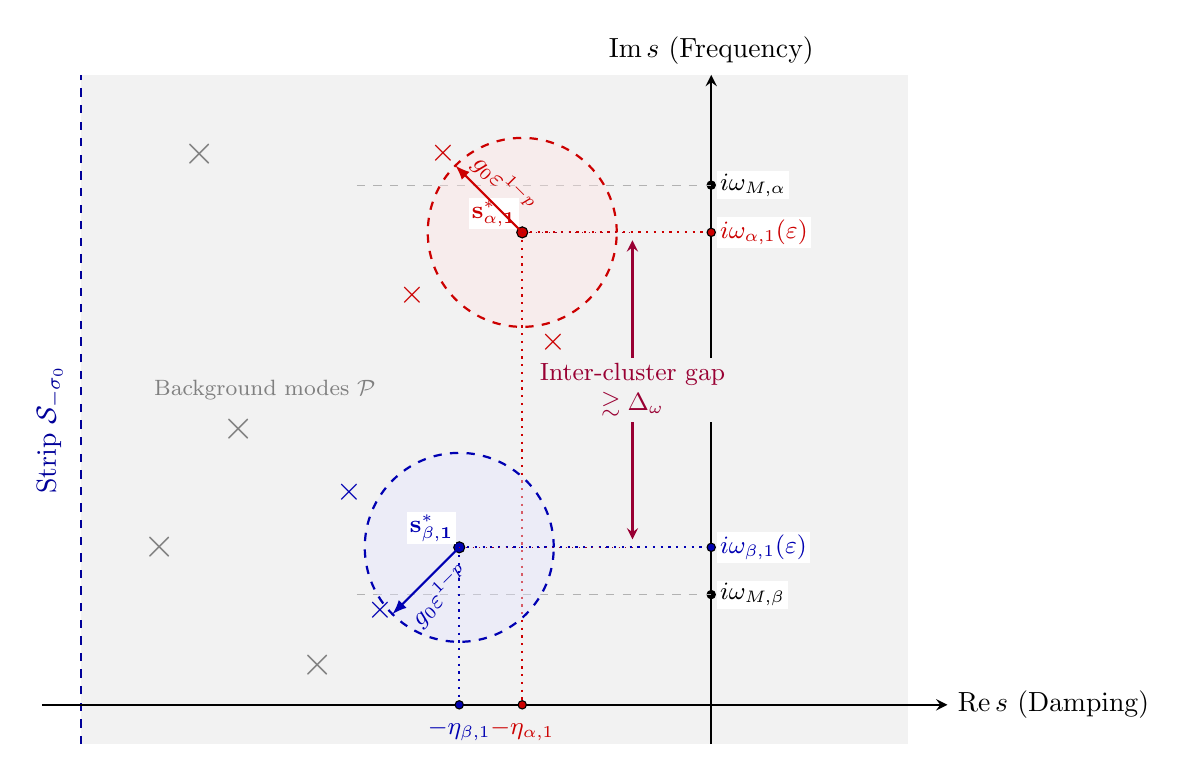
\begin{tikzpicture}[scale=1.0]

    % --- 1. SETTING THE BOUNDARIES & PARAMETERS ---
    \def\sigmaZero{-8.0}  
    
    % Unperturbed Physical Minnaert Frequencies (Assumption 2)
    \def\omegaMalpha{6.6}     
    \def\omegaMbeta{1.4}     
    
    % Cluster Alpha (Perturbed)
    \def\xAlpha{-2.4}  % Real part (-\eta_{\alpha, 1})
    \def\yAlpha{6.0}   % Imag part (\omega_{\alpha, 1})
    
    % Cluster Beta (Perturbed)
    \def\xBeta{-3.2}   % Real part (-\eta_{\beta, 1})
    \def\yBeta{2.0}    % Imag part (\omega_{\beta, 1})
    
    % The subwavelength isolation gap radius (g_0 \varepsilon^{1-p})
    \def\gap{1.2}        

    % --- 2. THE MEROMORPHIC STRIP ---
    \fill[gray!10] (\sigmaZero, -0.5) rectangle (2.5, 8.0);
    \draw[dashed, blue!60!black, thick] (\sigmaZero, -0.5) -- (\sigmaZero, 8.0);
    \node[blue!60!black, rotate=90] at (\sigmaZero-0.4, 3.5) {Strip $\mathcal{S}_{-\sigma_0}$};

    % --- 3. AXES ---
    \draw[-stealth, line width=0.8pt] (-8.5, 0) -- (3.0, 0) node[right] {$\Re s$ (Damping)};
    \draw[-stealth, line width=0.8pt] (0, -0.5) -- (0, 8.0) node[above] {$\Im s$ (Frequency)};

    % --- 4. UNPERTURBED BARE FREQUENCIES (Spectral Detuning) ---
    % Alpha unperturbed
    \draw[fill=black] (0, \omegaMalpha) circle (1.5pt);
    \node[right=2pt, font=\small, fill=white, inner sep=1pt] at (0, \omegaMalpha) {$i\omega_{M,\alpha}$};
    \draw[dashed, gray!60] (-4.5, \omegaMalpha) -- (0, \omegaMalpha);
    
    % Beta unperturbed
    \draw[fill=black] (0, \omegaMbeta) circle (1.5pt);
    \node[right=2pt, font=\small, fill=white, inner sep=1pt] at (0, \omegaMbeta) {$i\omega_{M,\beta}$};
    \draw[dashed, gray!60] (-4.5, \omegaMbeta) -- (0, \omegaMbeta);

    % --- 5. CLUSTER ALPHA ---
    % Isolation Gap (Exclusion Zone)
    \draw[thick, red!80!black, dashed, fill=red!10, fill opacity=0.4] (\xAlpha, \yAlpha) circle (\gap);
    
    % The EXACT center pole
    \draw[fill=red!80!black] (\xAlpha, \yAlpha) circle (2pt);
    \node[above left=1pt, fill=white, inner sep=1pt, font=\small, text=red!80!black] at (\xAlpha, \yAlpha) {$\mathbf{s_{\alpha, 1}^*}$};
    
    % Radius arrow (Microscopic isolation)
    \draw[-latex, thick, red!80!black] (\xAlpha, \yAlpha) -- ++(135:\gap) 
        node[midway, sloped, above=-1pt, font=\small] {$g_0 \varepsilon^{1-p}$};

    % Imaginary projection (Perturbed frequency)
    \draw[dotted, thick, red!80!black] (\xAlpha, \yAlpha) -- (0, \yAlpha);
    \draw[fill=red!80!black] (0, \yAlpha) circle (1.5pt);
    \node[right=2pt, font=\small, fill=white, inner sep=1pt, text=red!80!black] at (0, \yAlpha) {$i\omega_{\alpha, 1}(\varepsilon)$};

    % Real projection (Radiation damping)
    \draw[dotted, thick, red!80!black] (\xAlpha, \yAlpha) -- (\xAlpha, 0);
    \draw[fill=red!80!black] (\xAlpha, 0) circle (1.5pt);
    \node[below=2pt, font=\small, text=red!80!black] at (\xAlpha, 0) {$-\eta_{\alpha, 1}$};

    % Other microscopic poles in Cluster Alpha
    \node[scale=1.2, red!80!black] at (-3.4, 7.0) {$\times$};
    \node[scale=1.2, red!80!black] at (-3.8, 5.2) {$\times$};
    \node[scale=1.2, red!80!black] at (-2.0, 4.6) {$\times$};

    % --- 6. CLUSTER BETA ---
    % Isolation Gap (Exclusion Zone)
    \draw[thick, blue!70!black, dashed, fill=blue!10, fill opacity=0.4] (\xBeta, \yBeta) circle (\gap);

    % The EXACT center pole
    \draw[fill=blue!70!black] (\xBeta, \yBeta) circle (2pt);
    \node[above left=1pt, fill=white, inner sep=1pt, font=\small, text=blue!70!black] at (\xBeta, \yBeta) {$\mathbf{s_{\beta, 1}^*}$};
    
    % Radius arrow (Microscopic isolation)
    \draw[-latex, thick, blue!70!black] (\xBeta, \yBeta) -- ++(225:\gap) 
        node[midway, sloped, below=-1pt, font=\small] {$g_0 \varepsilon^{1-p}$};

    % Imaginary projection (Perturbed frequency)
    \draw[dotted, thick, blue!70!black] (\xBeta, \yBeta) -- (0, \yBeta);
    \draw[fill=blue!70!black] (0, \yBeta) circle (1.5pt);
    \node[right=2pt, font=\small, fill=white, inner sep=1pt, text=blue!70!black] at (0, \yBeta) {$i\omega_{\beta, 1}(\varepsilon)$};

    % Real projection (Radiation damping)
    \draw[dotted, thick, blue!70!black] (\xBeta, \yBeta) -- (\xBeta, 0);
    \draw[fill=blue!70!black] (\xBeta, 0) circle (1.5pt);
    \node[below=2pt, font=\small, text=blue!70!black] at (\xBeta, 0) {$-\eta_{\beta, 1}$};

    % Other microscopic poles in Cluster Beta
    \node[scale=1.2, blue!70!black] at (-4.2, 1.2) {$\times$};
    \node[scale=1.2, blue!70!black] at (-4.6, 2.7) {$\times$};

    % --- 7. MACROSCOPIC CLUSTER ISOLATION (Delta_omega) ---
    \draw[<->, thick, purple!80!black, >=stealth] (-1.0, \yBeta+0.1) -- (-1.0, \yAlpha-0.1)
        node[midway, fill=gray!10, inner sep=2pt, font=\small, align=center] {Inter-cluster gap\\$ \gtrsim \Delta_\omega$};
    \draw[dotted, purple!80!black] (\xAlpha, \yAlpha) -- (-1.0, \yAlpha);
    \draw[dotted, purple!80!black] (\xBeta, \yBeta) -- (-1.0, \yBeta);

    % --- 8. BACKGROUND SPECTRUM ---
    \foreach \p in {(-6.5, 7.0), (-6.0, 3.5), (-5.0, 0.5), (-7.0, 2.0)}{
        \node[gray, scale=1.5] at \p {$\times$};
    }
    \node[gray, left=4pt, font=\footnotesize] at (-4.0, 4) {Background modes $\mathcal{P}$};

\end{tikzpicture}
\caption{Schematic representation of the pole distribution for the transfer matrix $H_b(s)$ in the complex $s$-plane.} 
    \label{fig:pole-structure-multi-cluster-perfect}
\end{figure}


\begin{proposition}[Pole Structure and Minnaert Resonance]\label{proposition}
  Under Assumption \ref{assum:dual-scale-geometry}, and assuming that the physical input operator $B^{\mathrm{in}}(s)$ is analytic in $\mathbb{C}$, the microscopic transfer matrix $H_b(s)$ defined in \eqref{eq:Hb-definition} satisfies the following properties:
\begin{enumerate}[(i)]
    \item \big(\textit{Meromorphic structure of the transfer matrix}\big) 
    
    The transfer matrix $H_b(s)$ admits a meromorphic continuation to $\mathbb{C}$. In particular, it is meromorphic in the half-plane $$\mathcal{S}_{-\sigma_0} := \Big\{s \in \mathbb{C} : \Re(s) > -\sigma_0\Big\},$$ and its poles are contained in $\Big\{s : \det\big(\mathcal{D}(s)+s^2\mathcal{Q}(s,\varepsilon)\big) = 0\Big\}$.

   \item \big(\textit{Discrete Poles and Asymptotic Cluster Separation}\big)
 
   Let $\mathcal{P}$ denote the discrete set of poles of $H_b$ within $\mathcal{S}_{-\sigma_0}$. Due to the macroscopic material detuning, the dominant principal mode of each cluster $\alpha \in \Big\{1,2,\ldots,N\Big\}$ corresponds to a distinguished simple pole near its local unperturbed frequency $i\omega_{M,\alpha}$:$$s_{\alpha, 1}^\ast = -\eta_{\alpha, 1} + i\omega_{\alpha, 1}(\varepsilon), \quad \eta_{\alpha, 1}, \omega_{\alpha, 1}(\varepsilon) > 0.$$
   Moreover, there exists $\varepsilon_0 > 0$ and a constant $g_0 > 0$ such that for all $\varepsilon \in (0, \varepsilon_0]$, the pole $s_{\alpha, 1}^\ast$ is rigorously isolated from the complementary spectrum by an asymptotically scaled gap:$$\operatorname{dist}\bigl(s_{\alpha, 1}^\ast, \mathcal{P} \setminus \{s_{\alpha, 1}^\ast\}\bigr) \ge g_0 \varepsilon^{1-p} > 0.$$
   In addition to that the generic disjointness ($\omega_{M,\alpha} \ne \omega_{M,\beta}$), guarantees distinct cluster principle dominant poles are strictly isolated by an $\mathcal{O}(1)$ spectral distance, quantified as:
\begin{equation}
    |s_{M,\alpha}^\ast(\varepsilon) - s_{M,\beta}^\ast(\varepsilon)| = |\omega_{M,\alpha} - \omega_{M,\beta}| + \mathcal{O}(\varepsilon^{1-p}) \ge \Delta_\omega > 0,
\end{equation}
where $\Delta_\omega := \frac{1}{2} \min\limits_{\omega_{M,\beta} \neq \omega_{M,\alpha}} |\omega_{M,\alpha} - \omega_{M,\beta}|$.

    \item \big(\textit{Residue Expansion at the Distinguished Pole}\big)

    Assuming the $m$-th resonant mode of cluster $\alpha$ is not annihilated by the input/output projections, $H_b(s)$ admits a strict Laurent expansion in the neighborhood $U$ of $s_{\alpha, m}^\ast$:
    $$H_b(s) = \frac{R_{\alpha, m}}{s-s_{\alpha, m}^\ast} + H_{\mathrm{reg}}(s),$$
    where the residue $R_{\alpha, m} \in \mathbb{C}^{M \times M} \setminus \{\mathbf{0}\}$ and $H_{\mathrm{reg}}(s)$ is bounded and analytic in $U$. 
    %\rankrev{For an individual principal pole, the residue is associated with the corresponding principal cluster mode. Consequently, the relevant finite-rank object for the control problem is not an $M$-dimensional residue of all microscopic bubble variables. It is the residue obtained after restricting to the dominant subspace $E_{\mathrm{dom}}$ in \eqref{eq:dominant-cluster-subspace} and projecting onto the effective cluster source strengths. This compressed dominant residue has rank $N$ when the $N$ principal cluster modes are independently excitable and observable.}
\end{enumerate}
\end{proposition}
\begin{proof}
    See Section \ref{proofprop} for the details.
\end{proof}


\begin{assumption}[Cluster-level transducer accessibility]
\label{ass:transducer-accessibility}
Let $\mathcal K_{\rm tr}\Subset(0,\infty)$ be a compact frequency set containing the operational Minnaert bands
\[
    I_M=\bigcup_{\alpha=1}^N I_\alpha(\varepsilon)
\]
introduced below. For transducer locations $x_m^{\mathrm{tr}}$ ($1 \le m \le M_{\mathrm{tr}}$) and macroscopic cluster centers $y_\alpha$ ($1 \le \alpha \le N$), define the cluster-level trace matrix $\widetilde{G}_{\mathrm{tr}}(s) \in \mathbb{C}^{N \times M_{\mathrm{tr}}}$ via
\begin{equation}
\label{eq:Gtr-tilde-assumption}
    \widetilde{G}_{\mathrm{tr}}(s) := \bigl(G_s(y_\alpha,x_m^{\mathrm{tr}})\bigr)_{1\le \alpha\le N,\;1\le m\le M_{\mathrm{tr}}} ,
\end{equation}
We assume $M_{\mathrm{tr}} \ge N$ and the transducer geometry satisfies the uniform lower bound
\begin{equation}
\label{eq:Gtr-tilde-full-rank}
    \inf_{\omega\in\mathcal{K}_{\mathrm{tr}}} \sigma_{\min}\bigl(\widetilde{G}_{\mathrm{tr}}(i\omega)\bigr) \ge c_{\mathrm{tr}} > 0 .
\end{equation}
\end{assumption}

\bigskip

\noindent
The geometric condition \eqref{eq:Gtr-tilde-full-rank} holds for sufficiently distant transducers $x_m^{\mathrm{tr}} = R_m \theta_m$ ($R_m \gg 1$, $\theta_m \in \mathbb{S}^2$). Indeed, the far-field expansion 
$$G_{i\omega}(y_\alpha,x_m^{\mathrm{tr}}) = c_m(\omega) e^{i(\omega/c_0)\theta_m\cdot y_\alpha} + \mathcal{O}(R_m^{-1}),$$
with $c_m(\omega) \neq 0$, shows that $\widetilde{G}_{\mathrm{tr}}$ asymptotically acts as a multi-static sampling far-field response matrix for point sources at the cluster centers (well known in MUSIC-type algorithms). The underlying patterns $\{e^{i(\omega/c_0)\theta \cdot y_\alpha}\}_{\alpha=1}^N$ are linearly independent on $\mathbb{S}^2$; otherwise, Rellich's lemma and unique continuation would force the associated radiating field to vanish identically outside the cluster centers, contradicting the point singularities at $y_\alpha$. Consequently, a choice of $M_{\mathrm{tr}} \ge N$ distinct directions ensures $\operatorname{rank}(\widetilde{G}_{\mathrm{tr}}) = N$, a property that persists uniformly on $\mathcal{K}_{\mathrm{tr}}$ for large finite $R_m$.
\\
\noindent
The microscopic trace matrix $G_{\mathrm{tr}}(s) := \bigl(G_s(z_i,x_m^{\mathrm{tr}})\bigr) \in \mathbb{C}^{M\times M_{\mathrm{tr}}}$ satisfies
\begin{equation}
\label{eq:Gtr-cluster-perturbation}
  G_s(z_i,x_m^{\rm tr})=G_s(y_\alpha,x_m^{\rm tr})+\mathcal O(r_\varepsilon),
  \qquad
  r_\varepsilon:=\max_\alpha\max_{i\in\mathcal I_\alpha}|z_i-y_\alpha|,
\end{equation}
for all $i \in \mathcal{I}_\alpha$ and $s \in i\mathcal{K}_{\mathrm{tr}}$. Let $V_{\mathrm{dom}}^\varepsilon, W_{\mathrm{dom}}^\varepsilon \in \mathbb{C}^{M\times N}$ denote the biorthogonal principal cluster modes, satisfying $(W_{\mathrm{dom}}^\varepsilon)^\ast V_{\mathrm{dom}}^\varepsilon = I_N$. By the pole expansion of $H_b(s)$, the principal part of $\mathcal{H}_{\mathrm{ext}}^\varepsilon(s)$ on $I_M$ evaluates to
\begin{equation}
\label{eq:Hdom-explicit-definition}
    H_{\mathrm{dom}}^\varepsilon(s) := B_{\mathrm{out}} V_{\mathrm{dom}}^\varepsilon \operatorname{diag}\left(\frac{r_\alpha^\varepsilon}{s-s_{M,\alpha}^\ast}\right)_{\alpha=1}^N (W_{\mathrm{dom}}^\varepsilon)^\ast G_{\mathrm{tr}}(s) .
\end{equation}
Provided these modes are non-annihilated by the input-output projections, the macroscopic rank condition \eqref{eq:Gtr-tilde-full-rank} and the $\mathcal{O}(r_\varepsilon)$ trace perturbation ensure a uniform spectral bound. Specifically, for sufficiently small $\varepsilon$ and all $\omega \in I_M$, there exists $c_{\mathrm{ext}} > 0$ such that
\begin{equation}
\label{eq:Hext-smin-lower}
    \sigma_{\min}\bigl(\mathcal{H}_{\mathrm{ext}}^\varepsilon(i\omega)\bigr) \ge c_{\mathrm{ext}}\frac{\varepsilon}{\eta_{\max}} \ge c > 0,
\end{equation}
where $\eta_{\max} = \mathcal{O}(\varepsilon)$ is the maximal radiation damping scale. This guarantees a uniformly bounded right inverse for the physical control operator on the operational bands.



\begin{comment}
    \begin{assumption}[Cluster-level transducer accessibility]
\label{ass:transducer-accessibility}
\rankrev{Let $\mathcal K_{\rm tr}\Subset(0,\infty)$ be a compact frequency set containing the operational Minnaert bands
\[
    I_M=\bigcup_{\alpha=1}^N I_\alpha(\varepsilon)
\]
introduced below. Let $x_m^{\rm tr}$, $m=1,\dots,M_{\rm tr}$, be the transducer locations and let $y_\alpha$, $\alpha=1,\dots,N$, be the macroscopic cluster centers. We define the cluster-level transducer trace matrix
\begin{equation}
\label{eq:Gtr-tilde-assumption}
    \widetilde G_{\rm tr}(i\omega)
    :=\bigl(G_{i\omega}(y_\alpha,x_m^{\rm tr})\bigr)_{1\le \alpha\le N,\;1\le m\le M_{\rm tr}}
    \in\mathbb C^{N\times M_{\rm tr}} .
\end{equation}
We assume that the transducer geometry is chosen so that
\begin{equation}
\label{eq:Gtr-tilde-full-rank}
    \inf_{\omega\in\mathcal K_{\rm tr}}
    \sigma_{\min}\bigl(\widetilde G_{\rm tr}(i\omega)\bigr)
    \ge c_{\rm tr}>0 .
\end{equation}
\bigskip

\noindent This is a purely geometric condition: the incident fields generated by the transducers distinguish and independently excite the $N$ cluster centers. In particular, one must have $M_{\rm tr}\ge N$. For transducers placed sufficiently far from the active region, the entries of $\widetilde G_{\rm tr}$ take the asymptotic form
\[
    G_{i\omega}(y_\alpha,x_m^{\rm tr})
    =c_m(\omega)e^{i(\omega/c_0)\theta_m\cdot y_\alpha}+\mathcal O(R_m^{-1}),
    \qquad c_m(\omega)\ne0,
\]
where $R_m=|x_m^{\rm tr}|$ and $\theta_m=x_m^{\rm tr}/R_m$ after translating the active region into a bounded set. Thus, up to non-zero column factors and lower-order errors, $\widetilde G_{\rm tr}$ is a multi-static sampling far-field response matrix for point sources at the cluster centers (well known in MUSIC-type algorithms). The corresponding continuous far-field patterns are linearly independent. Indeed, a non-trivial linear combination vanished on the unite sphere $\mathbb S^2$, Rellich's lemma and unique continuation would imply that the radiating field generated by the associated point sources vanishes away from the points $y_\alpha$, which is impossible because of the remaining point singularities. Hence one can choose $M_{\rm tr}\ge N$ transducer directions so that the sampled matrix has full row rank. In addition, the same rank property persists for sufficiently large finite transducer distances and on compact frequency sets. The way in which \eqref{eq:Gtr-tilde-full-rank} combines with the microscopic resonant cluster analysis to give the right inverse used later is analyzed in Appendix~\ref{app:transducer-accessibility}.}
\end{assumption}
\end{comment}

\subsection{Spectral Isolation and Generic Controllability}
\noindent
Let $\Lambda := \{\hat{\omega}_\ell\}_{\ell=1}^L$ denote distinct Dirichlet angular eigenfrequencies, with eigenspaces $H_\ell := \operatorname{span}\{\phi_\ell^{(j)}\}_{j=1}^{m_\ell}$. Then, the global target subspace $H_M$ and its total dimension $N_M$ are constructed as follows:
$$H_M := \bigoplus_{\ell=1}^L H_\ell, \quad N_M := \sum_{\ell=1}^L m_\ell.$$
Following Assumption~\ref{assum:dual-scale-geometry}, we take $N \ge N_M$ macroscopic clusters centered at $\mathbf{y} = (y_1, \dots, y_N) \in \Omega^N$. Let $\tau: \{1,\dots,N\} \twoheadrightarrow \{1,\dots,L\}$ be a surjective map. The parameters of cluster $\alpha$ are tuned such that its principal perturbed Minnaert pole satisfies $\Im(s^\ast_{M,\alpha}(\varepsilon)) = \hat{\omega}_{\tau(\alpha)}$. 



\begin{proposition}[Spectral Isolation]
\label{ass:target-Dirichlet}
Let $I_\alpha(\varepsilon) := [\hat{\omega}_{\tau(\alpha)} - \delta(\varepsilon), \hat{\omega}_{\tau(\alpha)} + \delta(\varepsilon)]$ with $\delta(\varepsilon) \in \left(0, \frac{g_0}{2} \varepsilon^{1-p}\right)$. Then, we have
\begin{equation}
    \operatorname{dist}\bigl(I_\alpha(\varepsilon), \{\omega_k\}_{k\ge1} \setminus \{\hat{\omega}_{\tau(\alpha)}\}\bigr) \ge \frac{\Delta_\omega}{2} > 0, \quad \forall \alpha \in \{1,\dots,N\},
\end{equation}
where $\Delta_\omega > 0$ is the uniform macroscopic spectral gap.
\end{proposition}

\begin{proof}
    The proposition follows trivially from Step 6 of Proposition \ref{proposition}(ii) and the strict separation of the Dirichlet eigenvalues. $\hfill \blacksquare$
\end{proof}

\noindent
We define the composite Minnaert resonant band as the union of these isolated local bands ($I_\alpha \cap I_\beta = \emptyset$ for $\alpha \neq \beta$):
\begin{equation}
    I_M := \bigcup_{\alpha=1}^N I_\alpha(\varepsilon).
\end{equation}

\noindent
Given an orthonormal basis $\Psi := (\psi_1, \dots, \psi_{N_M})^\top$ of $H_M$, define the spatial coupling matrix $C_M(\mathbf{y}) \in \mathbb{R}^{N_M \times N}$ by $[C_M(\mathbf{y})]_{i\alpha} := \psi_i(y_\alpha)$.

\begin{proposition}[Generic Rank Condition]
\label{prop:generic-rank-CM}
For $N \ge N_M$, $\operatorname{rank}(C_M(\mathbf{y})) = N_M$ for Lebesgue almost every macroscopic cluster configuration $\mathbf{y} \in \Omega^N$.
\end{proposition}
\begin{proof}
We begin by defining $F: \Omega^{N_M} \to \mathbb{R}$ by $F(y_1, \dots, y_{N_M}) := \det(\psi_i(y_j))_{i,j=1}^{N_M}$. The real-analyticity of Dirichlet eigenfunctions in $\Omega$ implies $F$ is real-analytic. Because $\{\psi_i\}_{i=1}^{N_M}$ are linearly independent in $L^2(\Omega)$, $F \not\equiv 0$. Therefore, the zero set $\mathcal{Z}_{N_M} := F^{-1}(0)$ constitutes an analytic variety of Lebesgue measure zero, \cite[Ch. 6, Th. 6.3.3]{krantz2002primer}. For any $\mathbf{y} \in (\Omega^{N_M} \setminus \mathcal{Z}_{N_M}) \times \Omega^{N-N_M}$, the leading $N_M \times N_M$ principal submatrix of $C_M(\mathbf{y})$ is invertible.
\end{proof}

\noindent
Proposition \ref{prop:generic-rank-CM} formally embeds the localized problem into the classical framework of finite-dimensional exact controllability \cite[Ch. 1]{TucsnakWeissBook}. The Galerkin projection onto $H_{I_M}$ reduces the second-order wave dynamics to a first-order LTI system \begin{align}
    \dot{z}(t) = Az(t) + B(\mathbf{y})u(t)
\end{align}
on the state space $\mathbb{R}^{2N_M}$, where $z = (\mathbf{p}^\top, \dot{\mathbf{p}}^\top)^\top$. The system operator is the block matrix $A = \left(\begin{smallmatrix} 0 & I \\ -c_0^2\Lambda & 0 \end{smallmatrix}\right)$ with spectrum $\sigma(A) = \{\pm i c_0\omega_k\}_{k=1}^{N_M}$, and the input operator is $B(\mathbf{y}) = \left(\begin{smallmatrix} 0 \\ c_0^2 C_M(\mathbf{y}) \end{smallmatrix}\right)$. By the Hautus test \cite[Sec. 1.5]{TucsnakWeissBook}, exact controllability requires 
\begin{align}
    \operatorname{rank}\Big[\lambda I_{2N_M} - A \mid B(\mathbf{y})\Big] = 2N_M
\end{align}
for all $\lambda \in \mathbb{C}$. Given the block structures of $A$ and $B(\mathbf{y})$, this block-matrix rank condition is algebraically equivalent to the requirement that $$\operatorname{rank}(C_M(\mathbf{y})) = N_M.$$ 
The real-analyticity of the Dirichlet eigenfunctions ensures that the rank-deficient configurations form a proper analytic variety $\mathcal{Z}_{N_M}$. Consequently, its Lebesgue measure is zero ($\mathcal{L}(\mathcal{Z}_{N_M}) = 0$), strictly guaranteeing that the Hautus rank condition is generically satisfied.
\bigskip

\noindent Let us also mention that for simple geometries for $\Omega$, as cubes, one can give appropriate distributions of the macroscopic centers $y_\alpha$ so that the matrix $C_M$ is full rank, see Appendix of \cite{RodriguesSiniHeat}.

\begin{assumption}[Subspace Controllability]
\label{ass:Minnaert-coupling}
Assume $\mathbf{y} \notin \mathcal{Z}_{N_M} \times \Omega^{N-N_M}$. Consequently, we have $$\operatorname{rank}(C_M(\mathbf{y})) = N_M,$$ ensuring the existence of a uniformly bounded right inverse $L_M \in \mathbb{R}^{N \times N_M}$ satisfying $C_M(\mathbf y)L_M=I_{N_M}$.
\end{assumption}

%\rankrev{We shall keep the following notation throughout the realization part. The integer $M$ denotes the total number of microscopic bubbles, $N$ denotes the number of macroscopic clusters, $N_M:=\dim H_M$ denotes the dimension of the target Dirichlet subspace, and $M_{\rm tr}$ denotes the number of exterior transducers. These quantities play different roles. The spatial controllability condition concerns the matrix $C_M(\mathbf y)\in\mathbb R^{N_M\times N}$ and therefore requires $N\ge N_M$ and $\operatorname{rank}C_M(\mathbf y)=N_M$. The exterior accessibility condition concerns the physical map from the $M_{\rm tr}$ transducer signals to the $N$ dominant cluster channels.}

\begin{definition}[Multi-band source space on a finite time interval]
\label{def:multi-band-source-space}
Let
\[
        I_M=\bigcup_{\alpha=1}^N I_\alpha(\varepsilon)
\]
be the separated union of the operational Minnaert bands. Since the control problem is posed on the finite time interval $[0,T]$, we define the componentwise band space by restriction from the real line. Namely, $q=(q_1,\ldots,q_N)$ belongs to $V_{I_M}$ if, for every $\alpha =1,2,\ldots,N$, there exists an extension $\widetilde q_\alpha\in H^1(\mathbb R)$ such that
\[
        \widetilde q_\alpha|_{[0,T]}=q_\alpha,
        \qquad
        \operatorname{supp}\widehat{\widetilde q_\alpha}
        \subset I_\alpha(\varepsilon).
\]
We use the induced norm from $V=H^1(0,T;\mathbb R^N)$. Thus $V_{I_M}$ should be read as a finite-time, multi-channel restriction of globally band-limited source profiles.
\end{definition}

\begin{proposition}[Approximate Surjectivity on the Minnaert Band]
\label{prop:surjectivity-IM-statement}
Let $V_{I_M} \subset V$ be the multi-channel band space of Definition~\ref{def:multi-band-source-space}. The $\alpha$-th effective cluster-source component has temporal content in the band attached to the $\alpha$-th cluster. Because the bands are separated, $V_{I_M}$ is the direct product of the componentwise band-pass spaces corresponding to $I_\alpha(\varepsilon)$. For any fixed $T>0$, there exist constants $\varepsilon_0, \beta, C_T > 0$ and a family of bounded linear operators $R_{I_M}^\varepsilon \in \mathcal{L}(V_{I_M}, U_{\rm tr})$ for $\varepsilon \in (0, \varepsilon_0)$ satisfying:
\begin{align}
    &\sup_{\varepsilon \in (0, \varepsilon_0)} \|R_{I_M}^\varepsilon\|_{\mathcal{L}(V_{I_M}, U_{\rm tr})} < \infty, \label{eq:uniform-bound-IM} \\
    &\| \mathcal{T}^\varepsilon R_{I_M}^\varepsilon q - q \|_{V} \le C_T \varepsilon^\beta \| q \|_V, \quad \forall q \in V_{I_M}. \label{eq:approx-right-inverse-IM}
\end{align}
\end{proposition}
\begin{proof}
    See Section \ref{appsur} for the details.
\end{proof}


\subsection{Quantitative Estimation of the Intra-Cluster Spectral Gap}
\noindent
While Proposition~\ref{proposition}(ii) establishes the qualitative separation of the dominant pole (the Perron--Frobenius eigenvalue) from the sub-radiant modes within a given cluster, this section provides a rigorous quantitative characterization of their precise spectral configuration.
\newline
Let cluster $\alpha$ consist of $M_\alpha$ bubbles with a spatial scaling $d_{ij} = \widetilde{d}_{ij} \varepsilon^p$ for $p \in (0,1)$. Evaluating the interaction kernel at the unperturbed Minnaert resonance $s = i\omega_{M,\alpha}$ yields the leading-order operator:
\begin{equation}
    \widetilde{C}_\alpha^{(0)} := \lim_{\varepsilon \to 0} \varepsilon^{p-1} \mathcal{Q}(i\omega_{M,\alpha}, \varepsilon) = \frac{\mathcal{C}_\alpha}{4\pi} \mathcal{M}_\alpha,
\end{equation}
where $\mathcal{M}_\alpha$ is the dimensionless interaction matrix with entries:
\begin{equation}
    [\mathcal{M}_\alpha]_{ij} = (1 - \delta_{ij})\widetilde{d}_{ij}^{-1}.
\end{equation}
By Kato's analytic perturbation theory \cite{kato1995perturbation}, the principal resonance shift is dictated by the spectral radius $\mu_1(\alpha) = \max \sigma(\mathcal{M}_\alpha)$, which is a simple eigenvalue by the Perron--Frobenius theorem \cite[Ch. 8]{la1}. Driven by the qualitative properties established in Proposition~\ref{proposition}(ii), these principal frequencies $\omega_{\alpha, 1}$ are well-separated by design to closely approximate the target Dirichlet eigenvalues, yielding the asymptotic expansion:
\begin{equation} \label{eq:fine_shift}
    \omega_{\alpha, 1}(\varepsilon) = \omega_{M,\alpha} - \frac{\omega_{M,\alpha}^3 \mathcal{C}_\alpha}{8\pi} \mu_1(\alpha) \varepsilon^{1-p} + \mathcal{O}(\varepsilon^{\min(1, 2-2p)}).
\end{equation}
Since $\operatorname{Tr}(\mathcal{M}_\alpha) = 0$, isolating the principal pole $s_{\alpha, 1}^\ast$ requires a strictly positive spectral gap $\Delta\mu_\alpha := \mu_1(\alpha) - \mu_2(\alpha) > 0$. This defines the physical intra-cluster gap:
\begin{equation}
    \Delta_{\text{gap}}^{(\alpha)}(\varepsilon) := \frac{\omega_{M,\alpha}^3 \mathcal{C}_\alpha}{8\pi} \Delta\mu_\alpha \varepsilon^{1-p}.
\end{equation}
We explicitly quantify $\Delta\mu_\alpha$ for two physical arrangements:
\begin{enumerate}[(i)]
    \item \textit{Equidistant Cluster:} For uniform dimensionless distances $\widetilde{d}_{ij}=1$ (physically limited to $M_\alpha \le 4$ for embeddings in $\mathbb{R}^3$, representing a regular tetrahedron), the interaction matrix simplifies to $\mathcal{M}_\alpha = \mathbf{J} - \mathbf{I}$. The spectrum is $\sigma(\mathcal{M}_\alpha) = \{M_\alpha-1, -1, \dots, -1\}$, yielding a discrete gap $\Delta\mu_\alpha = M_\alpha > 0$.
     \item \textit{1D Uniform Lattice:} For a linear chain with spacing $h_\alpha$, the distance is $\widetilde{d}_{ij} = h_\alpha |i-j\|$. This reduces $\mathcal{M}_\alpha$ to a scaled symmetric Toeplitz matrix $h_\alpha^{-1}\mathcal{T}^{(\alpha)}$ with entries:
    \begin{equation}
        [\mathcal{T}^{(\alpha)}]_{ij} = (1 - \delta_{ij})|i-j|^{-1}.
    \end{equation}
    By standard row-sum bounds for non-negative matrices \cite{la1}, the spectral radius $\mu_1(\mathcal{T}^{(\alpha)})$ satisfies:
    \begin{equation}
        H_{M_\alpha-1} \le \mu_1(\mathcal{T}^{(\alpha)}) \le 2 H_{\lfloor M_\alpha/2 \rfloor}, \quad H_n := \sum_{k=1}^n k^{-1}.
    \end{equation}
    Furthermore, because the matrix $\mathcal{T}^{(\alpha)}$ is entrywise non-negative and irreducible (having strictly positive off-diagonal entries), the Perron--Frobenius theorem \cite[Ch. 8]{la1} ensures that its largest eigenvalue is unique and strictly separated from the second eigenvalue, guaranteeing a positive spectral gap:
    \begin{equation}
        C_{\alpha} := \mu_1(\mathcal{T}^{(\alpha)}) - \mu_2(\mathcal{T}^{(\alpha)}) > 0.
    \end{equation}
\end{enumerate}
Imposing the bandwidth restriction $\delta(\varepsilon) \in \left(0, \frac{1}{2} \min_\alpha \Delta_{\text{gap}}^{(\alpha)}(\varepsilon)\right)$ therefore rigorously isolates the principal pole $s_{\alpha, 1}^\ast$ from all sub-radiant modes.




\begin{figure}[H]
    \centering
    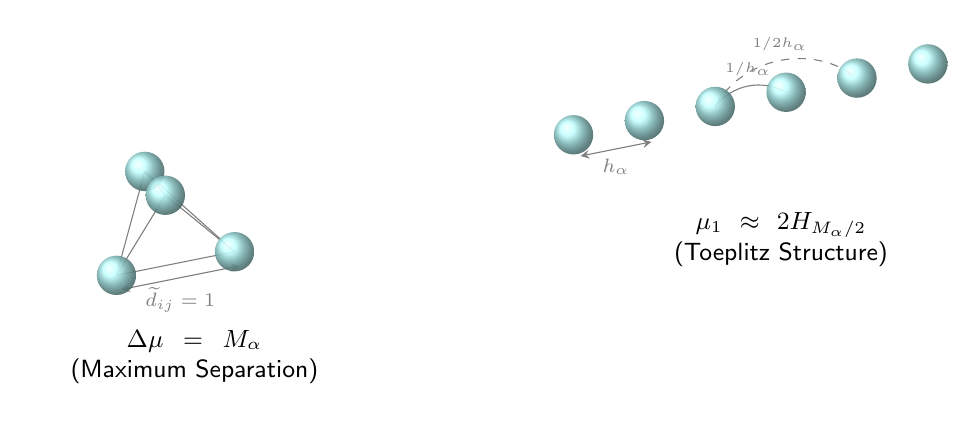
\begin{tikzpicture}[
        x={(1cm, 0.2cm)},
        y={(-0.3cm, 0.9cm)},
        z={(0cm, 0.4cm)},
        >=stealth,
        font=\small\sffamily
    ]

% --- Styles ---
\tikzset{
    bubble/.style={ball color=cyan!30, opacity=0.9},
    conn/.style={gray, thin},
    dist/.style={gray, <->, font=\scriptsize}
}

% --- Situation 1: Complete Graph K4 (Tetrahedron) ---
\begin{scope}[shift={(0,0,0)}]
    % Unified Title Position
    %\node[anchor=south, font=\bfseries] at (0.75, 2.5, 0) {1. Complete Graph $K_4$};
    
    % Coordinates for a regular tetrahedron
    \coordinate (A) at (0,0,0);
    \coordinate (B) at (1.5,0,0);
    \coordinate (C) at (0.75, 1.3, 0);
    \coordinate (D) at (0.75, 0.43, 1.2);

    % Connections (Edges)
    \draw[conn] (A) -- (B) -- (C) -- (A);
    \draw[conn] (A) -- (D); \draw[conn] (B) -- (D); \draw[conn] (C) -- (D);

    % Distance Label
    \draw[dist] ($(A)-(0,0.2,0)$) -- ($(B)-(0,0.2,0)$) node[midway, below] {$\widetilde{d}_{ij}=1$};

    % Nodes
    \foreach \p in {A,B,C,D} \shade[bubble] (\p) circle (0.25cm);
    
    \node[text width=4cm, align=center, below] at (0.75, -0.8, 0) {
        $\Delta\mu = M_\alpha$ \\ (Maximum Separation)};
\end{scope}

% --- Situation 2: 1D Uniform Lattice (Toeplitz) ---
% Added y-shift of 0.65 to center it vertically against the Tetrahedron
\begin{scope}[shift={(6, 0.65, 0)}]
    % Unified Title Position
    %\node[anchor=south, font=\bfseries] at (2.2, 2.5, 0) {2. 1D Uniform Lattice};

    \def\h{0.9} % spacing
    \foreach \i in {0,...,5} {
        \coordinate (P\i) at (\i*\h, 0, 0);
    }

    % Interaction decay visualization for center node
    \draw[conn, bend left=40] (P2) to node[midway, above, font=\tiny] {$1/h_\alpha$} (P3);
    \draw[conn, bend left=50, dashed] (P2) to node[midway, above, font=\tiny] {$1/2h_\alpha$} (P4);

    % Distance Label
    \draw[dist] ($(P0)-(0,0.3,0)$) -- ($(P1)-(0,0.3,0)$) node[midway, below] {$h_\alpha$};

    % Nodes
    \foreach \i in {0,...,5} \shade[bubble] (P\i) circle (0.25cm);

    \node[text width=4cm, align=center, below] at (2.2, -1.45, 0) {
        $\mu_1 \approx 2H_{M_\alpha/2}$ \\ (Toeplitz Structure)};
\end{scope}

\end{tikzpicture}
    \caption{Cluster topologies: (Left) physical equidistant cluster and (Right) 1D uniform lattice with Toeplitz interaction structure.}
    \label{fig:cluster_geometries}
\end{figure}



\begin{comment}
    \noindent
Let the system contain a total of $M$ bubbles partitioned into $N$ clusters. Let cluster $\alpha \in \{1, \dots, N\}$ comprise $M_\alpha$ bubbles (such that $\sum_{\alpha=1}^N M_\alpha = M$) with uniform capacitance $\mathcal{C}_\alpha$ and unperturbed Minnaert frequency $\omega_{M,\alpha}$. The intra-cluster distances $d_{ij} = \widetilde{d}_{ij} \varepsilon^p$ ($p \in (0,1)$) define the geometric graph $G_\alpha = (V_\alpha, E_\alpha)$. Evaluating the interaction matrix at $s = i\omega_{M,\alpha}$:
\begin{equation}
    \mathcal{Q}_{ij}(i\omega_{M,\alpha}, \varepsilon) = \varepsilon \frac{\mathcal{C}_\alpha}{4\pi \widetilde{d}_{ij} \varepsilon^p} e^{-i\frac{\omega_{M,\alpha}}{c_0} \widetilde{d}_{ij} \varepsilon^p} = \varepsilon^{1-p} \frac{\mathcal{C}_\alpha}{4\pi \widetilde{d}_{ij}} + \mathcal{O}(\varepsilon).
\end{equation}
Defining the leading-order operator $\widetilde{C}_\alpha^{(0)} := \lim_{\varepsilon \to 0} \varepsilon^{p-1} \mathcal{Q}(i\omega_{M,\alpha}, \varepsilon)$, we obtain strict proportionality to the reciprocal distance (Harary) matrix $RD(G_\alpha)$ \cite{cui_liu_harary}:
\begin{equation}
    \widetilde{C}_\alpha^{(0)} = \frac{\mathcal{C}_\alpha}{4\pi} RD(G_\alpha),
\end{equation}
where 
\begin{equation}
    \big[RD(G_\alpha)\big]_{ij} = \begin{cases} 
      \frac{1}{\widetilde{d}_{ij}} & \text{if } i \neq j, \\
      0 & \text{if } i = j.
   \end{cases}
\end{equation}
By Kato's analytic perturbation theory \cite{kato1995perturbation}, the principal perturbed frequency shifts proportionally to the Harary spectral radius $\mu_1(G_\alpha)$:
\begin{equation} \label{eq:fine_shift}
    \omega_{\alpha, 1}(\varepsilon) = \omega_{M,\alpha} - \frac{\omega_{M,\alpha}^3 \mathcal{C}_\alpha}{8\pi} \mu_1(G_\alpha) \varepsilon^{1-p} + \mathcal{O}(\varepsilon^{\min(1, 2-2p)}).
\end{equation}

\medskip
\noindent
\subsubsection{Inter-Cluster Disjointness and Degenerate Limit Bounds} 

\noindent
Define the macroscopic material detuning gap:
\begin{equation}
    \Delta_\omega := \frac{1}{2} \min_{\alpha \neq \beta} |\omega_{M,\alpha} - \omega_{M,\beta}| \ge 0.
\end{equation}
By the triangle inequality applied to $s_{M,\alpha}^\ast(\varepsilon) = -\eta_{\alpha, 1} + i\omega_{\alpha, 1}(\varepsilon)$:
\begin{equation}
    |s_{M,\alpha}^\ast(\varepsilon) - s_{M,\beta}^\ast(\varepsilon)| \ge |\omega_{M,\alpha} - \omega_{M,\beta}| - \mathcal{O}(\varepsilon^{1-p}) \ge 2\Delta_\omega - \mathcal{O}(\varepsilon^{1-p}).
\end{equation}
For non-degenerate materials ($\Delta_\omega > 0$), disjointness holds trivially as $\varepsilon \to 0$. 

\medskip
\noindent
\textit{Degenerate Limit ($\Delta_\omega \to 0$):} Assume $\omega_{M,\alpha} = \omega_{M,\beta} = \omega_M$ and $\mathcal{C}_\alpha = \mathcal{C}_\beta = \mathcal{C}$. To guarantee spectral separation, we engineer the clusters using distinct geometric graph topologies:
\begin{enumerate}[(a)]
    \item \textit{Complete Graph ($K_{M_\alpha}$):} A configuration where all $M_\alpha$ bubbles in cluster $\alpha$ are mutually equidistant ($\widetilde{d}_{ij} = 1$ for all $i \neq j$).
    \item \textit{Complete Bipartite Graph ($K_{p,q}$):} A configuration for cluster $\beta$ partitioned into two disjoint subsets of sizes $p$ and $q$ ($p+q=M_\beta$). Bubbles only interact across the partitions.
\end{enumerate}
Imposing these heterogeneous topologies ($G_\alpha \cong K_{M_\alpha}$ and $G_\beta \cong K_{p,q}$ with $M_\alpha, M_\beta \ge 3$), the spectral separation is bounded by the Harary topological variance:
\begin{equation}
    \inf_{\Delta_\omega \to 0} |s_{M,\alpha}^\ast(\varepsilon) - s_{M,\beta}^\ast(\varepsilon)| \ge \frac{\omega_M^3 \mathcal{C}}{8\pi} \left| \mu_1(K_{M_\alpha}) - \max_{p+q=M_\beta} \mu_1(K_{p,q}) \right| \varepsilon^{1-p}.
\end{equation}
Substituting $\mu_1(K_{M_\alpha}) = M_\alpha - 1$ and the balanced bipartite supremum $\max \mu_1(K_{p,q}) \le \frac{3M_\beta-2}{4}$ \cite{cui_liu_harary}, the explicit minimum topological gap is strictly positive. In the absolute worst-case scenario where clusters have identical local sizes ($M_\alpha = M_\beta = \widehat{M}$), the bound yields:
\begin{equation}
    \inf_{\Delta_\omega \to 0} |s_{M,\alpha}^\ast(\varepsilon) - s_{M,\beta}^\ast(\varepsilon)| \ge \frac{\omega_M^3 \mathcal{C}}{8\pi} \left( \widehat{M} - 1 - \frac{3\widehat{M} - 2}{4} \right) \varepsilon^{1-p} = \frac{\omega_M^3 \mathcal{C} (\widehat{M} - 2)}{32\pi} \varepsilon^{1-p} > 0.
\end{equation}

\medskip
\noindent
\subsubsection{Intra-Cluster Spectral Gaps} 
\noindent
Since $\operatorname{Tr}(RD(G_\alpha)) = 0$, we have $\sum_{i=1}^{M_\alpha} \mu_i = 0$ \cite{cui_liu_harary}. To isolate the principal pole $s_{\alpha, 1}^\ast$, the internal spectral gap $\mu_1(G_\alpha) - \mu_2(G_\alpha)$ must be strictly positive.
\begin{enumerate}[(i)]
    \item Let $G_\alpha \cong K_{M_\alpha}$. The spectrum is $\sigma(RD(K_{M_\alpha})) = \{M_\alpha-1, -1, \dots, -1\}$. The eigenvalue gap is $\mu_1 - \mu_2 = M_\alpha$, yielding the physical intra-cluster gap:
    \begin{equation}
        \Delta_{\text{gap}}^{(\alpha)}(\varepsilon) := \frac{\omega_{M,\alpha}^3 \mathcal{C}_\alpha}{8\pi} \Big( \mu_1(K_{M_\alpha}) - \mu_2(K_{M_\alpha}) \Big) \varepsilon^{1-p} = \frac{\omega_{M,\alpha}^3 \mathcal{C}_\alpha}{8\pi} M_\alpha \varepsilon^{1-p} > 0.
    \end{equation}
    \item Let $G_\beta \cong K_{p,q}$. The bipartite spectrum implies a strictly positive internal separation $C_{p,q} := \mu_1(K_{p,q}) - \mu_2(K_{p,q}) > 0$, yielding:
    \begin{equation}
        \Delta_{\text{gap}}^{(\beta)}(\varepsilon) = \frac{\omega_{M,\beta}^3 \mathcal{C}_\beta}{8\pi} C_{p,q} \varepsilon^{1-p} > 0.
    \end{equation}
\end{enumerate}
Consequently, restricting the operational bandwidth to $\delta(\varepsilon) \in \left(0, \frac{1}{2} \min_\alpha \Delta_{\text{gap}}^{(\alpha)}(\varepsilon)\right)$ rigorously isolates the principal pole $s_{\alpha, 1}^\ast$ from all sub-radiant modes for any chosen topology.


\begin{figure}[htbp]
    \centering
    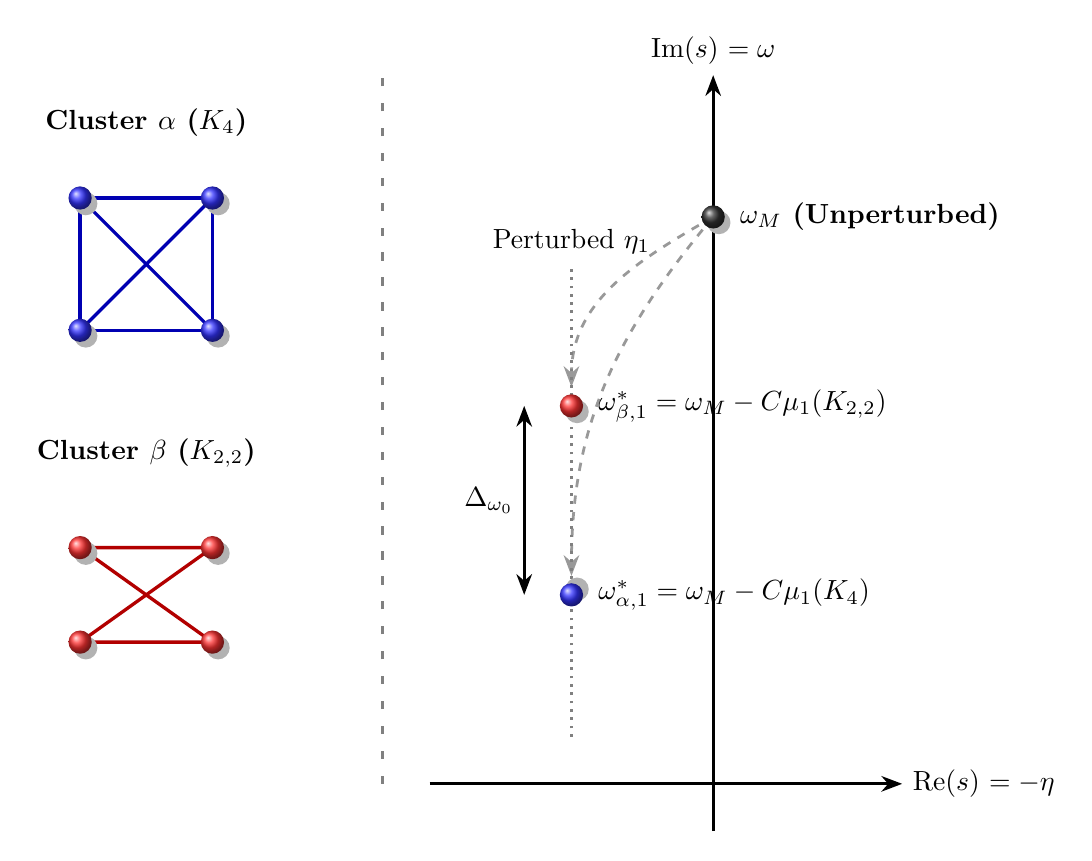
\begin{tikzpicture}[>=Stealth, thick, scale=1.2]

        % =========================================================
        % LEFT SIDE: PHYSICAL GRAPHS (3D Enhanced)
        % =========================================================
        
        % Cluster Alpha (K_4)
        \node[font=\bfseries] at (-3, 3) {Cluster $\alpha$ ($K_4$)};
        \begin{scope}[shift={(-3, 1.5)}]
            \coordinate (A1) at (-0.7, -0.7); \coordinate (A2) at (0.7, -0.7);
            \coordinate (A3) at (0.7, 0.7);   \coordinate (A4) at (-0.7, 0.7);
            
            % Edges
            \draw[blue!70!black, line width=1.2pt] (A1)--(A2)--(A3)--(A4)--cycle;
            \draw[blue!70!black, line width=1.2pt] (A1)--(A3) (A2)--(A4);
            
            % 3D Bubbles with shadows
            \foreach \n in {A1, A2, A3, A4} {
                % Drop shadow
                \fill[black!30] ($(\n) + (0.06, -0.06)$) circle (3.5pt);
                % 3D Sphere
                \shade[ball color=blue!80!white] (\n) circle (3.5pt);
            }
        \end{scope}

        % Cluster Beta (K_2,2)
        \node[font=\bfseries] at (-3, -0.5) {Cluster $\beta$ ($K_{2,2}$)};
        \begin{scope}[shift={(-3, -2)}]
            \coordinate (B1) at (-0.7, 0.5); \coordinate (B2) at (-0.7, -0.5);
            \coordinate (B3) at (0.7, 0.5);  \coordinate (B4) at (0.7, -0.5);
            
            % Edges
            \draw[red!70!black, line width=1.2pt] (B1)--(B3) (B1)--(B4) (B2)--(B3) (B2)--(B4);
            
            % 3D Bubbles with shadows
            \foreach \n in {B1, B2, B3, B4} {
                % Drop shadow
                \fill[black!30] ($(\n) + (0.06, -0.06)$) circle (3.5pt);
                % 3D Sphere
                \shade[ball color=red!80!white] (\n) circle (3.5pt);
            }
        \end{scope}

        % =========================================================
        % RIGHT SIDE: COMPLEX S-PLANE (3D Enhanced)
        % =========================================================
        
        \begin{scope}[shift={(3, 0)}]
            % Axes
            \draw[->, line width=1pt] (-3, -4) -- (2, -4) node[right] {Re($s$) $= -\eta$};
            \draw[->, line width=1pt] (0, -4.5) -- (0, 3.5) node[above] {Im($s$) $= \omega$};
            
            % Damping shift assumption
            \def\damping{-1.5}

            % Trajectories (Dashed lines showing movement from unperturbed)
            \draw[->, dashed, gray!80, line width=1pt] (0, 2) to[out=210, in=90] (\damping, 0.2);
            \draw[->, dashed, gray!80, line width=1pt] (0, 2) to[out=230, in=90] (\damping, -1.8);

            % Failsafe Gap Annotation
            \draw[<->, line width=1pt] (\damping - 0.5, 0) -- (\damping - 0.5, -2) 
                node[midway, left, font=\bfseries] {$\Delta_{\omega_0}$};
                
            % Damping line indicator
            \draw[dotted, gray, line width=1pt] (\damping, -3.5) -- (\damping, 1.5) node[above, text=black] {Perturbed $\eta_1$};

            % 3D Poles (Drawn last so they sit on top of the lines)
            
            % Unperturbed Pole (Black)
            \fill[black!30] (0.06, 1.94) circle (3.5pt); % Shadow
            \shade[ball color=black!80] (0, 2) circle (3.5pt) node[right=6pt, font=\bfseries] {$\omega_M$ (Unperturbed)};
            
            % Beta Pole Shift (Red)
            \fill[black!30] (\damping + 0.06, -0.06) circle (3.5pt); % Shadow
            \shade[ball color=red!80!white] (\damping, 0) circle (3.5pt) node[right=6pt] {$\omega_{\beta,1}^\ast = \omega_M - C \mu_1(K_{2,2})$};
            
            % Alpha Pole Shift (Blue)
            \fill[black!30] (\damping + 0.06, -1.94) circle (3.5pt); % Shadow
            \shade[ball color=blue!80!white] (\damping, -2) circle (3.5pt) node[right=6pt] {$\omega_{\alpha,1}^\ast = \omega_M - C \mu_1(K_4)$};

        \end{scope}

        % Divider Line
        \draw[loosely dashed, gray, line width=1pt] (-0.5, -4) -- (-0.5, 3.5);

    \end{tikzpicture}
    \caption{pole trajectories in the $s$-plane: Differing Harary radii for $K_4$ and $K_{2,2}$ cause distinct frequency shifts, guaranteeing a gap ($\Delta_{\omega_0}$) even when initial frequencies match.}
    \label{fig:complex_plane_poles}
\end{figure}
\end{comment}



\subsection{Control Objective and Main Results}
\noindent
\textit{\textbf{Problem.}} \Big(Finite-dimensional tracking and efficient Minnaert realization\Big)
Given a final time $T > 0$, the target Dirichlet subspace $H_M$ associated with the composite Minnaert band $I_M$, and a prescribed reference trajectory $p_r^{I_M} \in C^3([0,T]; H_M)$:
\begin{enumerate}[(i)]
\item First construct the ideal cluster-source profile which gives exact tracking in the finite-dimensional Dirichlet spectral model. 
\item The physical question is then to realize this ideal profile by incident waves generated outside $\Omega$. 
\end{enumerate}
The main result below concerns the efficient case where the ideal profile is realized through the separated Minnaert channels, with a uniform control cost. More precisely, find a family of admissible controls $\{\lambda^\varepsilon\}_{\varepsilon > 0} \subset U_{\rm tr}$ such that the generated physical pressure fields $p^\varepsilon$ satisfy the uniform tracking condition:
\begin{equation*}
 \sup_{t\in[0,T]} 
 \Bigl( 
  \|P_{I_M} p^\varepsilon(\cdot,t) - p_r^{I_M}(\cdot,t)\|_{H^1(\Omega)} 
  + 
  \|P_{I_M} \partial_t p^\varepsilon(\cdot,t) - \partial_t p_r^{I_M}(\cdot,t)\|_{L^2(\Omega)} 
 \Bigr) 
 = \mathcal{O}(\varepsilon^\gamma)
\end{equation*}
for some constant $\gamma > 0$, subject to the uniform control cost bound:
\begin{equation*}
 \sup_{\varepsilon > 0} \|\lambda^\varepsilon\|_{U_{\rm tr}} < \infty.
\end{equation*}

\noindent
The following theorem should be read in this sense. The abstract finite-dimensional tracking step is valid for arbitrary sufficiently smooth trajectories in $H_M$. The additional spectral localization to $I_M$ enters only at the physical realization step: it is the condition under which the incident fields can generate the required ideal sources with uniformly bounded amplitudes. It is worth mentioning that the procedure suggested in this work is reconstructive.

\begin{comment}
    \begin{theorem}[Minnaert-Resonant Subspace Tracking]
\label{thm:Minnaert-tracking_main}
Let $T>0$. Define the physical control input space $U_{\rm tr}:=\{\lambda\in H^2(0,T; \mathbb{R}^{M_{\rm tr}}):\lambda(0)=\dot\lambda(0)=0\}$ and the effective dominant cluster-source space $V := H^1(0,T; \mathbb{R}^N)$. Let $I_M := \bigcup_{\alpha=1}^N I_\alpha(\varepsilon)$ be the composite Minnaert band and let $V_{I_M}\subset V$ be the finite-time multi-band source space of Definition~\ref{def:multi-band-source-space}. Let $H_M = \operatorname{span}\{\psi_k\}_{k=1}^{N_M} \subset L^2(\Omega)$ be the associated $N_M$-dimensional target Dirichlet subspace, with $N\ge N_M$ effective cluster channels. Let $P_{I_M}: L^2(\Omega) \to H_M$ denote the orthogonal projection onto this subspace. Consider:
\begin{enumerate}[(i)]
    \item \textit{Physical Asymptotics:} \rev{The configuration satisfies Material Parameter Scaling (Assump. \ref{as111}) and Topological Separation (Assump. \ref{assum:dual-scale-geometry}). The physical scattered field admits the decomposition $p^\varepsilon=p^{\mathrm{eff},\varepsilon}+\operatorname{err}_\varepsilon$ outside the bubbles, where $p^{\mathrm{eff},\varepsilon}$ is the $N$-cluster effective field obtained from the $M$-bubble retarded expansion by the cluster reduction of Section~\ref{sec:bubble-transfer}; see \eqref{eq:cluster-retarded-field}--\eqref{eq:cluster-effective-wave-Omega}. The projected remainder contains the original transmission-asymptotic error and the macroscopic cluster-reduction error, and is of order $\mathcal{O}(\varepsilon^\mu)$ in the regime considered.}
    \item \textit{Rank Condition:} The macroscopic cluster configuration $\mathbf{y} \in \Omega^N$ is generic (Prop. \ref{prop:generic-rank-CM}), strictly satisfying $\operatorname{rank}(C_M(\mathbf{y})) = N_M$.
    \item \textit{Operator Surjectivity:} \rankrev{By the pole expansion of Proposition~\ref{proposition}, the rank-$N$ dominant cluster-output structure, and the cluster-level transducer accessibility of Assumption~\ref{ass:transducer-accessibility}, Appendix~\ref{app:transducer-accessibility} yields the exterior-to-cluster lower singular-value estimate \eqref{eq:Hext-smin-lower}. Hence the physical actuator map admits a right inverse on the composite Minnaert band, denoted $H_{\mathrm{dom}}^\#$, satisfying}
 \[ 
  \rankrev{\sup_{\omega\in I_M}\|H_{\mathrm{dom}}^\varepsilon(i\omega)^{\#}\|_2 = \mathcal{O}\left(\frac{\eta_M}{\varepsilon}\right) \le \kappa_M < \infty.}
 \]
 \rankrev{Since $\eta_M\sim\varepsilon$, the physical actuator map from exterior transducer signals to dominant cluster-source outputs admits a right inverse $R_{I_M}^\varepsilon$ uniformly bounded by $$\sup_{\varepsilon > 0} \|R_{I_M}^\varepsilon\|_{\mathcal{L}(V_{I_M},U_{\rm tr})} \le \kappa_M.$$ This conclusion uses the transducer accessibility condition \eqref{eq:Gtr-tilde-full-rank} together with the microscopic resonant cluster structure of Proposition~\ref{proposition}; it is not a consequence of pole separation alone.}
\end{enumerate}
 Thus, for the resonant realization, we consider an ideal effective source profile $q^{\mathrm{ideal}} \in V_{I_M} \subset V$ that precisely generates the target reference field $p_r^{I_M} \in C^2([0,T]; H_M)$, which uniquely solves the ideal Dirichlet spectral wave equation:
\begin{equation}\label{ref-pressure}
    \left(\frac{1}{c_0^2}\partial_{tt} - \Delta_D\right) p_r^{I_M}(x,t) = \textcolor{red}{P_{I_M}} \sum_{\alpha=1}^N q^{\mathrm{ideal}}_\alpha(t)\delta_{y_\alpha}(x), \quad (x,t) \in \Omega \times (0,T].
\end{equation}
{\color{revisionmagenta}We impose the compatible rest initial conditions
\begin{equation}
  p^{\mathrm{eff},\varepsilon}(\cdot,0)=0, \quad \partial_t p^{\mathrm{eff},\varepsilon}(\cdot,0)=0, \quad
  p_r^{I_M}(\cdot,0)=0, \quad \partial_t p_r^{I_M}(\cdot,0)=0.
\end{equation}}
\rev{Let $p^{\mathrm{eff},\varepsilon}$ be the effective pressure generated by the realized cluster-level source vector $q^\varepsilon=\mathcal{T}^\varepsilon\lambda^\varepsilon$, and let $p^\varepsilon$ denote the corresponding physical scattered pressure, so that $p^\varepsilon=p^{\mathrm{eff},\varepsilon}+\operatorname{err}_\varepsilon$ in the projected/asymptotic sense described above. Then, $\exists \varepsilon_0, \gamma, \beta, C_T > 0$ (independent of $\varepsilon$) such that $\forall \varepsilon \in (0,\varepsilon_0)$, the explicit control $\lambda^\varepsilon := R_{I_M}^\varepsilon q^{\mathrm{ideal}} \in U_{\rm tr}$ yields the uniform tracking bound:}
\begin{equation}
\label{eq:Minnaert-tracking-final}
 \sup_{t\in[0,T]}
 \Bigl(
  \|P_{I_M} (p^\varepsilon - p_r^{I_M})(\cdot,t)\|_{H^1(\Omega)}
  +
  \|P_{I_M} \partial_t (p^\varepsilon - p_r^{I_M})(\cdot,t)\|_{L^2(\Omega)}
 \Bigr)
 \le C_T\,\varepsilon^\gamma.
\end{equation}
Furthermore, the physical control cost satisfies the strictly bounded uniform estimate:
\begin{equation}
  \|\lambda^\varepsilon\|_{U_{\rm tr}} \le \kappa_M \|q^{\mathrm{ideal}}\|_V.
\end{equation}
\end{theorem}
\end{comment}




\begin{theorem}[Minnaert-Resonant Subspace Tracking]
\label{thm:Minnaert-tracking_main}
 Let $T>0$. Define the physical control input space $U_{\mathrm{tr}} := \{\boldsymbol{\lambda} \in H^2(0,T; \mathbb{R}^{M_{\mathrm{tr}}}) : \boldsymbol{\lambda}(0) = \dot{\boldsymbol{\lambda}}(0) = \mathbf{0}\}$ and the effective cluster-source space $V := H^1(0,T; \mathbb{R}^N).$ Let $I_M := \bigcup_{\alpha=1}^N I_\alpha(\varepsilon)$ be the composite Minnaert band, $V_{I_M}\subset V$ be the multi-band source space, and $H_M = \operatorname{span}\{\psi_k\}_{k=1}^{N_M} \subset L^2(\Omega)$ be the $N_M$-dimensional target Dirichlet subspace ($N\ge N_M$) with orthogonal projection $P_{I_M}: L^2(\Omega) \to H_M$. 
\newline
Assume the foundational Material Parameter Scaling (Assump. \ref{as111}), Topological Separation (Assump. \ref{assum:dual-scale-geometry}), and Transducer Accessibility (Assump. \ref{ass:transducer-accessibility}) hold. Under these assumptions, the following properties are established in the
Minnaert-resonant regime:
\begin{enumerate}[(i)]
    \item \textit{Asymptotic Field Decomposition:} The physical scattered field satisfies the decomposition $p^\varepsilon = p^{\mathrm{eff},\varepsilon} + \operatorname{err}_\varepsilon$ on $\Omega \setminus \overline{D}$, where the projected remainder obeys the uniform estimate:
    \begin{equation}
    \label{eq:f-eps-H-1}
        \sup_{t\in[0,T]} \Bigl( \|P_{I_M}\operatorname{err}_{\varepsilon}(\cdot,t)\|_{H^1(\Omega\setminus \overline{D})} + \|P_{I_M}\partial_t\operatorname{err}_{\varepsilon}(\cdot,t)\|_{L^2(\Omega\setminus \overline{D})} \Bigr) \le C_T\varepsilon^\mu,
    \end{equation}
    with $p^{\mathrm{eff},\varepsilon}$ be the effective pressure generated by the realized cluster-level source vector $q^\varepsilon=\mathcal{T}^\varepsilon\lambda^\varepsilon.$
    \item \textit{Rank Condition:} The macroscopic cluster configuration $\mathbf{y} \in \Omega^N$ is generic (Prop. \ref{prop:generic-rank-CM}), strictly satisfying $\operatorname{rank}(C_M(\mathbf{y})) = N_M$.
    \item \textit{Frequency-Domain Solvability and Surjectivity:} By the Pole Structure (Prop. \ref{proposition}), the exterior-to-cluster transfer matrix $\mathcal{H}_{\mathrm{ext}}^\varepsilon(i\omega)$ has full row rank $N$ for all $\omega\in I_M$ with radiation damping $\eta_{\max} \sim \varepsilon$. Its pseudo-inverse satisfies the uniform frequency-domain bound (Prop. \ref{prop:surjectivity-IM}):
    \begin{equation}
    \label{eq:Hext-right-inverse-bound-thm}
        \sup_{\omega\in I_M} \|\bigl(\mathcal{H}_{\mathrm{ext}}^\varepsilon(i\omega)\bigr)^\dagger\|_2 \le C\frac{\eta_{\max}}{\varepsilon} \le \kappa_0 < \infty,
    \end{equation}
    ensuring that the physical actuator map $\mathcal{T}^\varepsilon: U_{\mathrm{tr}} \to V$ admits a right inverse $R_{I_M}^\varepsilon$ satisfying the uniform time-domain cost estimate:
    \begin{equation}
        \|R_{I_M}^\varepsilon\|_{\mathcal{L}(V_{I_M},U_{\mathrm{tr}})} \le \kappa_M.
    \end{equation}
\end{enumerate}
Consequently, let $\mathbf{q}^{\mathrm{ideal}} \in V_{I_M}$ be an ideal source profile generating the reference trajectory $p_r^{I_M} \in C^{\textcolor{red}{3}}([0,T]; H_M)$ via the ideal Dirichlet spectral wave equation:
\begin{equation}\label{ref-pressure}
    \left(\frac{1}{c_0^2}\partial_{tt} - \Delta_D\right) p_r^{I_M}(x,t) = P_{I_M} \sum_{\alpha=1}^N q^{\mathrm{ideal}}_\alpha(t)\delta_{y_\alpha}(x), \quad (x,t) \in \Omega \times (0,T],
\end{equation}
subject to compatible rest initial conditions $$p^{\mathrm{eff},\varepsilon}(\cdot,0) = \partial_t p^{\mathrm{eff},\varepsilon}(\cdot,0) = 0\ \text{and} \ p_r^{I_M}(\cdot,0) = \partial_t p_r^{I_M}(\cdot,0) = 0.$$ 
Then, there exist constants $\varepsilon_0, \gamma, C_T > 0$ independent of $\varepsilon$ such that for all $\varepsilon \in (0,\varepsilon_0)$, the explicit physical control vector $\boldsymbol{\lambda}^\varepsilon := R_{I_M}^\varepsilon \mathbf{q}^{\mathrm{ideal}} \in U_{\mathrm{tr}}$ yields a realized physical scattered pressure field $p^\varepsilon$ satisfying the uniform tracking bound:
\begin{equation}
\label{eq:Minnaert-tracking-final}
    \sup_{t\in[0,T]} \Bigl( \|P_{I_M} (p^\varepsilon - p_r^{I_M})(\cdot,t)\|_{H^1(\Omega\setminus \overline{D})} + \|P_{I_M} \partial_t (p^\varepsilon - p_r^{I_M})(\cdot,t)\|_{L^2(\Omega\setminus \overline{D})} \Bigr) \le C_T\,\varepsilon^\gamma,
\end{equation}
with an associated physical control cost bounded by 
$$\|\boldsymbol{\lambda}^\varepsilon\|_{U_{\mathrm{tr}}} \le \kappa_M \|\mathbf{q}^{\mathrm{ideal}}\|_V.$$  

\end{theorem}

\noindent In \eqref{ref-pressure}, \(P_{I_M}\delta_{y_\alpha}\) is defined by duality, namely $
P_{I_M}\delta_{y_\alpha}
:=
\sum_{k=1}^{N_M}\psi_k(y_\alpha)\psi_k ,
$
so that
$
\big\langle P_{I_M}\delta_{y_\alpha},\varphi\big\rangle
=
\varphi(y_\alpha), \varphi\in H_M .
$
Hence \eqref{ref-pressure} is an equation in \(H_M\).

\begin{remark}
We strictly require the target source profile to reside in the multi-band space $V_{I_M}$ to guarantee physical realizability at a bounded cost. While the ideal tracking construction holds for arbitrary trajectories, attempting to track temporal components outside the Minnaert resonance channels will result in a physical control cost that diverges as $\varepsilon \to 0$. The technical nuances of reconciling finite-time tracking with band-limited signal constraints are detailed in Section \ref{sec:resonant-gain}.
\end{remark}



 \begin{remark}[Comparison with Thermo--Plasmonic Heat Tracking]

While related to the thermo-plasmonic feedback framework in \cite{RodriguesSiniHeat}, the present setting differs mathematically in two fundamental ways. First, because the ideal PDE dynamics \eqref{eq:ideal-controlled-wave} are hyperbolic and conservative rather than parabolic, stabilization cannot rely on intrinsic semigroup decay; thus, tracking is strictly formulated on the finite spectral band $H_J$. Second, as used in \cite{RodriguesSiniHeat}, while plasmonic resonance merely improves the conditioning of the realization map, the Minnaert resonance rigorously dictates the \emph{gain} and invertibility of $H_b(s)$, rendering it the central enabler for effective pressure tracking.

\end{remark}




\paragraph{Tracking as an inverse problem for the control-to-state map.}
Once the dynamics are projected onto $H_M$, the actuation design problem becomes: find actuator signals (or, in the bubble realisation, the corresponding physical parameters) so that the modal coefficients of the solution match a prescribed reference $\bm p_r$ (either at a terminal time $T$ or over a time window). In operator form this amounts to solving a linear equation of the first kind on the finite-dimensional cluster-source space,
\[
 \mathcal{K}_M(\bm q)=\bm p_r,
\]
where $\mathcal{K}_M$ denotes the reduced control-to-state map induced by the projected wave propagator and the point-actuator coupling matrix $C_M=\big[\psi_k(y_\alpha)\big]$. Existence and robustness of tracking therefore \textcolor{red}{reduces to} the existence of a right-inverse of $\mathcal{K}_N$ with controlled norm (equivalently, on uniform conditioning of its matrix representation). The Minnaert regime improves this conditioning through resonant amplification of the bubble monopole response, whereas away from resonance the same inverse problem becomes ill-conditioned under the physical actuation constraints.

\subsection*{Organisation of the paper}
\noindent
The remainder of this paper is organised as follows. Section~\ref{sec:abstract-wave} formulates the wave equation with ideal point actuators, proving exact tracking for $C^3$ trajectories via the coupling matrix inverse $L_M$. Section~\ref{sec:bubble-R3} derives the time-domain asymptotic expansions and localises the scattered field model to the bounded domain $\Omega$. Section~\ref{proofprop} provides a meromorphic analysis of the bubble transfer matrix $H_b(s)$ and characterises the isolated Minnaert poles. Section~\ref{sec:resonant-gain} demonstrates the approximate surjectivity of the bubble actuator map on the resonant band, overcoming the non-resonant divergence problem. Section~\ref{sec:proof-main} proves the main tracking result (Theorem~\ref{thm:Minnaert-tracking_main}) using energy-based error estimates as $\varepsilon \to 0$. %Finally, Section~\ref{sec:gap-estimation} provides quantitative spectral gap estimations and discusses extensions to variable media and stabilization.

\section{Ideal Point-Actuator Tracking}
\label{sec:abstract-wave}
\noindent
In this section we formulate the controlled wave equation on $\Omega$ with point actuators at the macroscopic cluster centers $y_\alpha$, and prove an exact tracking result on a finite-dimensional spectral subspace. 

\subsection{Abstract formulation and well-posedness}
\noindent
We consider the point-actuated wave equation on a bounded domain $\Omega\subset\mathbb{R}^3$
with homogeneous Dirichlet boundary conditions. 
\begin{align}\label{eq:wave-control}
    \begin{cases}
        \dfrac{1}{c_0^2}\,\partial_t^2 p - \Delta p = \displaystyle\sum_{\alpha=1}^N q_\alpha(t)\,\delta_{y_\alpha}
        & \text{in }\Omega\times(0,T),\\
        p = 0 & \text{on }\partial\Omega\times(0,T),\\
        p(\cdot,0)=0,\quad \partial_t p(\cdot,0)=0.
    \end{cases}
\end{align}
In dimension three, the right-hand side does not belong to the dual of the standard energy space,
so \eqref{eq:wave-control} cannot be interpreted directly as a well-posed evolution problem in
$H^1_0(\Omega)\times L^2(\Omega)$. This problem can also be treated by transposition/duality in spaces associated with $D(-\Delta_D)'$, see \cite{KunischRodriguesWalter,MichielsNiculescu,TucsnakWeissBook}. Since we are interested here in a finite-dimensional tracking system, we therefore adopt a Galerkin (band-limited) formulation.
\newline
Let $\{\psi_k\}_{k\ge1}$ be the Dirichlet Laplacian eigenfunctions, forming an orthonormal basis of $L^2(\Omega)$, and let $H_M := \mathrm{span}\{\psi_1,\dots,\psi_{N_M}\}$ denote the $N_M$-dimensional target subspace corresponding to the macroscopic Minnaert composite band $I_M$, with orthogonal projection $P_{I_M} : L^2(\Omega)\to H_M$. Given the cluster-level source vector $\mathbf q=(q_1,\dots,q_N)^\top\in L^2(0,T;\mathbb R^N)$, we seek
\[
p_M(t)\in H_M,\qquad t\in[0,T],
\]
such that, for a.e.\ $t\in(0,T)$,
\begin{equation}
\label{eq:galerkin-weak}
 \frac{1}{c_0^2}\langle \partial_t^2 p_M(\cdot,t), \varphi\rangle
 + \langle \nabla p_M(\cdot,t), \nabla \varphi\rangle
 = \sum_{\alpha=1}^N q_\alpha(t)\,\varphi(y_\alpha),
 \qquad \forall \varphi\in H_M,
\end{equation}
with trivial projected initial data
\begin{equation}
\label{eq:IC-galerkin}
 p_M(\cdot,0)=0,\qquad \partial_t p_M(\cdot,0)=0.
\end{equation}
Since $H_M$ is finite-dimensional and spanned by smooth eigenfunctions, we have $H_M \subset H^2(\Omega)$, and in particular $\varphi(y_\alpha)$ is well-defined for all $\varphi\in H_M$. Hence the right-hand side of \eqref{eq:galerkin-weak} is strictly well-defined.

\begin{proposition}[Galerkin well-posedness from rest]
\label{prop:well-posed}
Let $T>0$ and $\mathbf q\in L^2(0,T;\mathbb R^N)$. Then the Galerkin problem
\eqref{eq:galerkin-weak}--\eqref{eq:IC-galerkin} admits a unique solution
\[
 p_M\in H^2(0,T;H_M).
\]
Writing $p_M(x,t)=\sum_{k=1}^{N_M} p_k(t)\psi_k(x)$, the coefficients satisfy the decoupled forced oscillator system
\begin{equation}
\label{eq:mode-ODE-N}
 \ddot p_k(t)+\omega_k^2 p_k(t)
 = c_0^2 \sum_{\alpha=1}^N q_\alpha(t)\psi_k(y_\alpha),
 \qquad k=1,\dots,N_M,
\end{equation}
with initial data $p_k(0)=0$ and $\dot p_k(0)=0$.
Moreover, there exists a constant $C_{T,M}>0$ (depending on $T$ and the target subspace $H_M$, but not on $\mathbf{q}$) such that the energy satisfies the bound
\begin{equation}
\label{eq:galerkin-energy-est}
 \sup_{t\in[0,T]}
 \Bigl(
  \norm{\nabla p_M(\cdot,t)}_{L^2(\Omega)}
  + \norm{\partial_t p_M(\cdot,t)}_{L^2(\Omega)}
 \Bigr)
 \le C_{T,M} \norm{\mathbf q}_{L^2(0,T;\mathbb R^N)}.
\end{equation}
\end{proposition}

\begin{proof}
Substituting the expansion $p_M(x,t)=\sum\limits_{k=1}^{N_M} p_k(t)\psi_k(x)$ into the weak formulation \eqref{eq:galerkin-weak} and choosing test functions $\varphi=\psi_k$, we obtain
\[
\frac{1}{c_0^2}\ddot p_k(t) + \lambda_k p_k(t)
= \sum_{\alpha=1}^N q_\alpha(t)\psi_k(y_\alpha).
\]
Multiplying by $c_0^2$ and setting $\omega_k^2=c_0^2\lambda_k$ yields \eqref{eq:mode-ODE-N}. Since $\psi_k\in C^\infty(\overline{\Omega})$, the quantities $\psi_k(y_\alpha)$ are well-defined. 
\newline
Introducing the modal vector $\bm p^M(t):=(p_1(t),\dots,p_{N_M}(t))^\top$, the diagonal matrix $\Lambda_M:=\mathrm{diag}(\omega_1^2,\dots,\omega_{N_M}^2)$, and the geometric modal evaluation matrix $C_M(\mathbf y)\in\mathbb R^{N_M\times N}$ with $[C_M(\mathbf y)]_{k\alpha}:=\psi_k(y_\alpha)$, the system can be written compactly as
\begin{equation}\label{eq:modal-matrix}
\ddot{\bm p}^M(t)+\Lambda_M\bm p^M(t)=c_0^2 C_M(\mathbf y)\mathbf q(t).
\end{equation}
This is a linear second-order ODE in $\mathbb{R}^{N_M}$ with $L^2$ forcing, and therefore admits a unique solution $\bm p^M\in H^2(0,T;\mathbb{R}^{N_M})$ subject to $\bm p^M(0)=0$ and $\dot{\bm p}^M(0)=0$. This implies $p_M\in H^2(0,T;H_M)$. 
\noindent
We now derive the energy estimate. Define the modified modal energy
\[
E_M(t):=\frac12\Bigl(|\Lambda_M^{1/2}\bm p^M(t)|^2+|\dot{\bm p}^M(t)|^2\Bigr).
\]
Differentiating and substituting the dynamics from \eqref{eq:modal-matrix}, we obtain
\[
E_M'(t)=\dot{\bm p}^M(t)\cdot (c_0^2 C_M(\mathbf y)\mathbf q(t)).
\]
By the Cauchy--Schwarz inequality and the matrix operator norm,
\[
E_M'(t)\le c_0^2 |\dot{\bm p}^M(t)|\,\|C_M(\mathbf y)\|\,|\mathbf q(t)|
\le c_0^2 \sqrt{2E_M(t)}\,\|C_M(\mathbf y)\|\,|\mathbf q(t)|.
\]
Setting $y(t):=\sqrt{E_M(t)}$ and noting $y(0)=0$, we obtain $y'(t)\le c_0^2 \|C_M(\mathbf y)\|\,|\mathbf q(t)|$ for a.e.\ $t\in(0,T)$. Integrating over $[0,t]$ yields
\[
\sup_{t\in[0,T]} y(t) \le c_0^2 \|C_M(\mathbf y)\|\sqrt{T}\,\|\mathbf q\|_{L^2(0,T;\mathbb R^N)}.
\]
Finally, noting that $|\dot{\bm p}^M(t)| = \|\partial_t p_M(\cdot,t)\|_{L^2(\Omega)}$ and translating the stiffness term via $\omega_k^2 = c_0^2\lambda_k$:
\[
|\Lambda_M^{1/2}\bm p^M(t)|^2 = \sum_{k=1}^{N_M} c_0^2\lambda_k |p_k(t)|^2 = c_0^2 \|\nabla p_M(\cdot,t)\|_{L^2(\Omega)}^2,
\]
the bounds on $y(t)$ directly establish \eqref{eq:galerkin-energy-est}. \hfill $\blacksquare$
\end{proof}

\begin{comment}
In the rest of the paper we work with homogeneous initial data for the wave
equation, in accordance with the setting of \cite{MukherjeeSiniJEE, MukherjeeSiniSIAM}, where the
incident fields are generated from sources with zero initial Cauchy data. Nonzero
initial data can be handled by superposition and do not affect the tracking
strategy on the spectral bands considered here.
\end{comment}

\subsection{Tracking on a finite spectral subspace}
\noindent
Let $T>0$ and $\bm{p}_r\in C^3([0,T];\R^{N_M})$ be a target reference trajectory for the modes in the Minnaert band. Define the corresponding reference field
\[
 p_r^{I_M}(x,t):=\sum_{k=1}^{N_M} (\bm{p}_r(t))_k\psi_k(x).
\]
Since the wave equation \eqref{eq:wave-control} starts from rest, we assume that the reference trajectory also starts from rest to ensure compatibility:
\begin{equation}
\label{eq:IC-match}
 (\bm{p}_r(0))_k=0,\qquad
 (\dot{\bm{p}}_r(0))_k= 0,\qquad k=1,\dots,N_M.
\end{equation}
\noindent
By Proposition \ref{prop:generic-rank-CM}, the macroscopic coupling matrix $C_M(\mathbf y)\in\mathbb R^{N_M\times N}$ has full row rank $N_M$ for $N\ge N_M$. Equivalently, there exists a right inverse $L_M\in\mathbb R^{N\times N_M}$ such that
\[
 C_M(\mathbf y)L_M=I_{N_M}.
\]

\begin{theorem}[Exact tracking on the target subspace]
\label{thm:finite-tracking}
Let $N \ge N_M$ and satisfy the generic rank condition. Let $T>0$ and $\bm{p}_r\in C^3([0,T];\R^{N_M})$ satisfying \eqref{eq:IC-match}. Define the ideal actuator control vector:
\begin{equation}
\label{eq:control-ideal}
 \mathbf{q}^{\mathrm{ideal}}(t):=\frac{1}{c_0^2} L_M \bigl(\ddot{\bm{p}}_r(t)+\Lambda_M\bm{p}_r(t)\bigr),\qquad t\in[0,T].
\end{equation}
Let $\bm{p}^M$ be the unique solution of \eqref{eq:modal-matrix} driven by $\mathbf{q}=\mathbf{q}^{\mathrm{ideal}}$ with zero initial data. Then
\[
 \bm{p}^M(t)=\bm{p}_r(t),\qquad
 \dot{\bm{p}}^M(t)=\dot{\bm{p}}_r(t),\qquad t\in[0,T],
\]
and consequently
\[
 P_{I_M} p(\cdot,t)=p_r^{I_M}(\cdot,t),\quad
 P_{I_M}\partial_t p(\cdot,t)=\partial_t p_r^{I_M}(\cdot,t),\quad t\in[0,T].
\]
\end{theorem}

\begin{proof}
By Proposition~\ref{prop:well-posed}, for any $\mathbf q\in L^2(0,T;\R^N)$ the system \eqref{eq:modal-matrix} admits a unique solution $\bm p^M\in H^2(0,T;\R^{N_M})$. In particular, the control \eqref{eq:control-ideal} is admissible since $\bm p_r\in C^3([0,T];\R^{N_M})$.
\newline
Using \eqref{eq:control-ideal} and the identity $C_M(\mathbf y)L_M=I_{N_M}$, we obtain
\[
 c_0^2 C_M(\mathbf y)\mathbf q^{\mathrm{ideal}}(t)
 =C_M(\mathbf y)L_M \bigl(\ddot{\bm{p}}_r(t)+\Lambda_M\bm{p}_r(t)\bigr)
 =\ddot{\bm{p}}_r(t)+\Lambda_M\bm{p}_r(t).
\]
Thus \eqref{eq:modal-matrix} becomes
\[
 \ddot{\bm{p}}^M(t)+\Lambda_M\bm{p}^M(t)
 =\ddot{\bm{p}}_r(t)+\Lambda_M\bm{p}_r(t),\qquad t\in[0,T].
\]
Define the tracking error $\bm{e}(t):=\bm{p}^M(t)-\bm{p}_r(t)$. Then $\bm e$ satisfies
\[
 \ddot{\bm{e}}(t)+\Lambda_M\bm{e}(t)=0,\qquad t\in[0,T],
\]
with initial conditions
\[
 \bm{e}(0)=0,\qquad \dot{\bm{e}}(0)=0,
\]
by \eqref{eq:IC-match}. Since this is a homogeneous linear ODE with constant coefficients, uniqueness implies $\bm e\equiv 0$ on $[0,T]$, which yields the result. \hfill $\blacksquare$
\end{proof}

\begin{remark}[Why we do not pursue feedback stabilization of the truncated wave system]\label{rem:no-feedback}
The reduced model \eqref{eq:modal-matrix} is a finite-dimensional, \emph{lossless} second-order system.
Thus, in open loop, the homogeneous error dynamics $\ddot{\bm e}+\Lambda_M \bm e=0$ conserve energy and
do not exhibit decay. For each fixed $N_M$, one could in principle add a feedback term (e.g. pole placement)
to render the closed-loop $N_M$-mode error exponentially stable.
We do not follow this route here for two reasons.

\smallskip
\noindent{\bf (i) Lack of uniformity as $N_M$ grows.}
Even when a stabilizing gain exists for each fixed $N_M$, the corresponding decay rates and gain bounds typically
deteriorate as $N_M\to\infty$ for wave dynamics with finitely many localized actuators. In particular, high-frequency
modes become increasingly difficult to control/observe, and there is in general no exponential decay estimate that is
\emph{uniform} in $N_M$; the required feedback gains may blow up as $N_M$ increases.

\smallskip
\noindent{\bf (ii) Spillover for the full PDE.}
A controller designed on the truncated system acts on the physical (infinite-dimensional) wave equation and may excite
unmodelled modes (the complement of $H_M$). In the absence of physical damping these components do not decay, so
stabilization of the truncated model does not automatically translate into stabilization of the full lossless PDE.

\smallskip
\noindent
Instead, our strategy is \emph{finite-horizon tracking} on the chosen mode set, as in Theorem~\ref{thm:finite-tracking},
combined with a physically realizable right-inversion step (Level 1) that produces the effective forcing coefficients from incident
fields. In the bubbly setting, the Minnaert resonance improves the gain/conditioning of this realization map, and hence
allows one to increase the number of tracked modes while keeping the actuation within feasible levels.
\end{remark}



\section{Bubble Dynamics and the Transfer Matrix}\label{sec:bubble-transfer}
\label{sec:bubble-R3}


\noindent
We now connect the ideal point-actuator model to the physical bubble model, in which the required effective sources are generated by external incident fields through a delayed, finite-dimensional multiple-scattering system.

\subsection{Scattered field as a superposition of retarded monopoles}
\label{subsec:time-domain-asymptotics}
\noindent
Recall the physical transmission problem \eqref{eq:MS-physical} defined in Section \ref{subsec:math-formulation}. The incident field in the homogeneous medium generated by the $M_{\rm tr}$ external transducers at $x_m^{\mathrm{tr}} \subset\R^3\setminus \overline{\Omega}$ with signals $\lambda \in U_{\rm tr}$ is given by the superposition:
\begin{equation}
\label{eq:incident-field-R3}
 u^{\mathrm{in}}(x,t)
 =
 \sum_{m=1}^{M_{\rm tr}}
 \frac{\rho_c}{4\pi|x-x_m^{\mathrm{tr}}|}
 \,\lambda_m\bigl(t-c_0^{-1}|x-x_m^{\mathrm{tr}}|\bigr).
\end{equation}
We follow the setting of \cite{MukherjeeSiniJEE,MukherjeeSiniSIAM}. Under the Assumptions \ref{as111} and  \ref{assum:dual-scale-geometry}, the scattered field $u^{\mathrm{sc}}:=u-u^{\mathrm{in}}$ admits a rigorous multipole expansion.



\begin{proposition}[Scattered field expansion and bubble system]
\label{prop:MS-expansion}
Under the Assumptions \ref{as111} and  \ref{assum:dual-scale-geometry} on the bubble geometry and the high-contrast scaling, there exist:
\begin{enumerate}
  \item constants $\mathcal{C}_i(\varepsilon)=\varepsilon \tilde{\mathcal{C}}_i$, where $\tilde{C}_i>0$ are constants independent of $\varepsilon$ and depending only on the geometry and contrasts of the bubble $D_i$;
  \item scalar functions $Y_i\in C^2([0,T])$, $i=1,\dots,M$, solving a finite-dimensional delayed system (see \eqref{eq:Y-tilde-system-vector} below);
  \item a remainder $R^\varepsilon\in C\big([0,T];L^2_{\mathrm{loc}}(\R^3\setminus \overline{D})\big)$;
\end{enumerate}
such that for $x$ in bounded regions away from the cluster,
\begin{equation}
\label{eq:MS-expansion-again}
 u^{\mathrm{sc}}(x,t)
 =
 -\sum_{i=1}^M C_i(\varepsilon)\,
 \frac{1}{4\pi|x-z_i|}
 \,Y_i\bigl(t-c_0^{-1}|x-z_i|\bigr)
 + R^\varepsilon(x,t),
 \qquad t\in[0,T],
\end{equation}
and, for the chosen bounded localization domain $\Omega$ containing all bubbles, there exist $\mu>0$ and $C_{T,\Omega}>0$ independent of $\varepsilon$ such that
\begin{equation}
\label{eq:R-eps-estimate-again}
 \textcolor{blue}{\sup_{t\in[0,T]}\norm{R^\varepsilon(\cdot,t)}_{L^2\big(\Omega\setminus \overline{D}\big)}
 \le C_{T,\Omega}\varepsilon^\mu.}
\end{equation}
Here, $\big(\mathrm{Y}_i\big)_{i=1}^M$ is the vector solution to the following non-homogeneous second-order matrix differential equation with zero initial conditions:
\begin{align}
\label{eq:Y-tilde-system}
    \begin{cases}
        \omega_M^{-2} \dfrac{\mathrm{d}^2}{\mathrm{d} t^2} \mathrm{Y}_i(t) + \mathrm{Y}_i(t) + \sum\limits_{\substack{j=1 \\ j \neq i}}^M q_{ij} \dfrac{\mathrm{d}^2}{\mathrm{d} t^2} \mathrm{Y}_j\bigl(t - \tau_{ij}\bigr) = \dfrac{\partial^2}{\partial t^2} u^\textit{in}(z_i,t), &\textit{in} \; (0, T), \\
        \mathrm{Y}_i(0) = \dfrac{\mathrm{d}}{\mathrm{d} t} \mathrm{Y}_i(0) = 0,
    \end{cases}
\end{align}
where $\omega_M^{-2} = \dfrac{\rho_c}{2 \overline{\kappa}_{\mathrm{b},i}} \Lambda_{\partial B_i}$ represents the inverse square of the Minnaert frequency $\omega_M$ of the bubble $D_i$ (see, for instance, \cite{Ammari-1, DGS-21}). For each $i=1,\dots,M$, the parameters satisfy
\begin{align*}
    \omega_M^{-2} > 0,
\qquad \tau_{ij} = c_0^{-1}|z_i - z_j| \ge 0 \ (j=1,\dots,M),
\qquad q_{ij} = \frac{C_j(\varepsilon)}{4\pi |z_i - z_j|} \in \mathbb R,
\end{align*}
with the convention $q_{ii} = 0$ and $\tilde{C}_j := \operatorname{vol}(B_j)\frac{\rho_c}{\overline{\kappa}_{\mathrm{b},j}}.$ Also, $\displaystyle\Lambda_{\partial B_i} := \frac{1}{|\partial B_i|} \int_{\partial B_i} \int_{\partial B_i}
 \frac{(\mathrm{x} - \mathrm{y}) \cdot \nu_\mathrm{x}}{|\mathrm{x} - \mathrm{y}|}
 \, d\sigma_\mathrm{x} \, d\sigma_\mathrm{y}$ is a geometric constant. The well-posedness of the system of differential equations \eqref{eq:Y-tilde-system} is discussed in \cite[Section 2.4]{MukherjeeSiniJEE}. In vector form, \eqref{eq:Y-tilde-system} can be written as
\begin{equation}
\label{eq:Y-tilde-system-vector}
 \mathbcal{D}\,\ddot{\mathrm{\bm{Y}}}(t)
 + \mathrm{Y}(t)
 + \mathbcal{Q}\bigl[\ddot{\mathrm{\bm{Y}}}\bigr](t)
 = \bm{\mathbcal{F}}(t),\qquad
 \mathrm{Y}(0)=\dot{\mathrm{Y}}(0)=0,
\end{equation}
where (i) $\mathbcal{D}:=\mathrm{diag}(d_1,\dots,d_M)$, (ii) $Q[\ddot{\mathrm{Y}}](t)$ has components
\[
 \bigl(\mathbcal{Q}[\ddot{\mathrm{Y}}](t)\bigr)_i
 :=\sum_{j\neq i}q_{ij}\,\ddot{\mathrm{Y}}_j\bigl(t-\tau_{ij}\bigr),
 \quad
 \tau_{ij}:=c_0^{-1}|z_i-z_j|,
\]
and (iii) $\bm{\mathbcal{F}}(t)\in\R^M$ has $i$-th component $\dfrac{\partial^2}{\partial t^2} u^\textit{in}(z_i,t)$.
\end{proposition}

\noindent
Define
\[
 q_i^\veps(t):=-C_i(\veps)\,\widetilde{Y}_i(t),\qquad i=1,\dots,M,
\]
and $q^\veps=(q_1^\veps,\dots,q_M^\veps)$. Then \eqref{eq:MS-expansion-again} becomes
\begin{equation}
\label{eq:retarded-actuators}
 u^{\mathrm{sc}}(x,t)
 =
 \sum_{i=1}^M
 \frac{1}{4\pi|x-z_i|}\,q_i^\veps\bigl(t-c_0^{-1}|x-z_i|\bigr)
 + R^\veps(x,t).
\end{equation}
Let us now introduce the retarded fundamental solution of the wave operator in the homogeneous medium:
\begin{equation}
\label{eq:fundamental-wave}
 \mathcal{G}_0(x,t;y)
 :=
 \frac{\rho_c}{4\pi|x-y|}\,\delta\bigl(t-c_0^{-1}|x-y|\bigr),
 \qquad x\neq y,\ t>0.
\end{equation}
Given a time-dependent source $f\in\mathscr{S}'(\R)$, the retarded field generated by a point source at $y\in\R^3$ is
\begin{equation}
\label{eq:def-W}
\mathcal{W}[f;y](x,t) := (\mathcal{G}_0(\cdot - y,\cdot) *_{t} f)(x,t)
= \frac{1}{4\pi |x-y|} \, f\!\left(t - c_0^{-1}|x-y|\right),
\end{equation}
where $f$ is extended by zero to negative times.
Equivalently, using the representation \eqref{eq:def-W}, we introduce the effective scattered pressure
\[
 p^{\mathrm{eff},\veps}(x,t)
 :=
 \sum_{i=1}^M \mathcal{W}[q_i^\veps;\,z_i](x,t).
\]
For given $T,$ we can find $\Omega, D\subset \Omega,$ such that the physical scattered field is then compared to this effective field by
\[
 u^{\mathrm{sc}}(x,t)=p^{\mathrm{eff},\veps}(x,t)+\operatorname{err}_{\veps}(x,t),
 \qquad (x,t)\in (\Omega\setminus\overline D)\times(0,T),
\]
where the asymptotic estimate controls $\operatorname{err}_{\veps}$ only away from the bubbles. Thus the following point-source equation is not asserted for the full physical field; it is the defining equation for the effective field:
\begin{equation}
\label{eq:effective-wave-R3}
 \frac{1}{c_0^2}\partial_t^2 p^{\mathrm{eff},\veps} - \Delta p^{\mathrm{eff},\veps}
 = \sum_{i=1}^M q_i^\veps(t)\,\delta_{z_i}
 \quad\text{in }\mathscr{D}'(\R^3\times(0,T)).
\end{equation}

\subsection{Cluster reduction and localization to the bounded domain $\Omega$}
\label{subsec:cluster-reduction-localization}
\noindent
Restricting the effective field to the bounded observation domain $\Omega$, one may first write the localized version of the $M$-bubble effective model as
\begin{equation}
\label{eq:effective-wave-Omega}
 \frac{1}{c_0^2}\partial_t^2 p^{\mathrm{eff},\veps}_{M} - \Delta p^{\mathrm{eff},\veps}_{M}
 = \sum_{i=1}^M q_i^\veps(t)\,\delta_{z_i}
 \quad\text{in }\Omega\times(0,T),
\end{equation}
understood after projection onto finite-dimensional Dirichlet spectral subspaces.
\newline
We now pass from the microscopic retarded representation to the cluster-output representation used by the control model. This is a reduction of the field representation, after the $M$-dimensional microscopic bubble system has determined the amplitudes $q_i^\veps$. Let
\[
 r_\veps:=\max_{1\le\alpha\le N}\max_{i\in\mathcal I_\alpha}|z_i-y_\alpha|
\]
be the maximal cluster diameter. On observation sets separated from the bubbles, the retarded kernel $\mathcal G_0(x,t;z)$ is smooth in the source variable $z$ for $z$ near each cluster. Hence, for $i\in\mathcal I_\alpha$,
\[
 \mathcal W[q_i^\veps;z_i]
 =\mathcal W[q_i^\veps;y_\alpha]+\mathcal O(r_\veps),
\]
with the error measured in the same away-from-the-bubbles norms as in \eqref{eq:MS-expansion-again}, provided the amplitudes are controlled in the corresponding time norms. Summing inside each cluster yields
\begin{equation}
\label{eq:cluster-retarded-field}
 p^{\mathrm{eff},\veps}_{M}(x,t)
 =
 \sum_{\alpha=1}^N \mathcal W[Q_\alpha^\veps;y_\alpha](x,t)
 +\mathcal R_{\rm cl}^\veps(x,t),
 \qquad
 Q_\alpha^\veps(t):=(B_{\rm out}\mathbf q_{\rm mic}^\veps(t))_\alpha
 =\sum_{i\in\mathcal I_\alpha}q_i^\veps(t).
\end{equation}
In the principal coherent Minnaert mode of cluster $\alpha$, one may write
\[
 q_i^\veps(t)=\widetilde q_\alpha^\veps(t)+\rho_i^\veps(t),
 \qquad i\in\mathcal I_\alpha,
\]
where $\rho_i^\veps$ denotes the non-dominant intra-cluster component. Consequently
\[
 Q_\alpha^\veps(t)=M_\alpha\widetilde q_\alpha^\veps(t)
 +\sum_{i\in\mathcal I_\alpha}\rho_i^\veps(t).
\]
Thus, on the selected principal cluster band, the effective cluster strength is $Q_\alpha^\veps\simeq M_\alpha\widetilde q_\alpha^\veps$, while $\mathcal R_{\rm cl}^\veps$ and the non-dominant components are included in the final physical remainder.
\newline 
Thus the localized actuator model used in the finite-dimensional tracking argument is the cluster-level effective model
\begin{equation}
\label{eq:cluster-effective-wave-Omega}
 \frac{1}{c_0^2}\partial_t^2 p^{\mathrm{eff},\veps}_{\rm cl} - \Delta p^{\mathrm{eff},\veps}_{\rm cl}
 = \sum_{\alpha=1}^N Q_\alpha^\veps(t)\delta_{y_\alpha}
 \quad\text{in }\Omega\times(0,T).
\end{equation}
In the rest of the paper, we write $q_\alpha^\veps$ for this cluster-level coefficient $Q_\alpha^\veps$ when no confusion is possible. Thus the symbol $q_\alpha$ in the ideal Dirichlet spectral model denotes the strength multiplying $\delta_{y_\alpha}$, not a single microscopic bubble amplitude. The physical field is then related to the effective one by
\begin{equation}
\label{eq:phys-eff-decomposition-Omega}
 p^\veps=p^{\mathrm{eff},\veps}+\operatorname{err}_{\veps}
 \quad\text{on }(\Omega\setminus\overline D)\times(0,T),
\end{equation}
and the only error estimate used in the control argument is the projected bound
\begin{equation}
\label{eq:f-eps-H-1}
 \sup_{t\in[0,T]}
 \Bigl(
 \norm{P_{I_M}\operatorname{err}_{\veps}(\cdot,t)}_{H^1(\Omega\setminus \overline{D})}
 +\norm{P_{I_M}\partial_t\operatorname{err}_{\veps}(\cdot,t)}_{L^2(\Omega\setminus \overline{D})}
 \Bigr)
 \le C_T\veps^\mu.
\end{equation}
This is the form compatible with the asymptotic result of the bubbly transmission problem: the control is designed for $p^{\mathrm{eff},\veps}$, and the physical pressure $p^\veps$ is recovered up to $\operatorname{err}_{\veps}$.

\begin{remark}[Dependence of the remainder on the excitation]
The bubbly transmission problem and the effective source amplitudes are linear in the incident excitation. In the estimates of \cite{MukherjeeSiniJEE,MukherjeeSiniSIAM}, the constants in projected remainder bounds such as \eqref{eq:f-eps-H-1} depend (at most) linearly on suitable norms of the incident field on $[0,T]$.
Accordingly, when designing controls it is important to keep
\(\|\lambda^\veps\|_{U_{\rm tr}}\) uniformly bounded (or at least polynomially bounded) with
respect to $\veps$, so that the asymptotic error remains of order
\(\mathcal{O}(\veps^\mu)\) on $[0,T]$.
This loop is closed in the Minnaert regime once a uniformly bounded (or
quantified) right inverse is available for the actuator map.
\end{remark}
\noindent
We shall work on $\Omega$ with the effective field $p^{\mathrm{eff},\veps}$ satisfying \eqref{eq:effective-wave-Omega}; the physical field is denoted by $p^\veps$ and is compared to $p^{\mathrm{eff},\veps}$ through \eqref{eq:phys-eff-decomposition-Omega}--\eqref{eq:f-eps-H-1}.

\subsection{Laplace-domain transfer function of the bubble subsystem}
\noindent
To control the effective sources $q^\varepsilon(t) \in V$, we must invert the dynamical relationship between the external transducers and the bubble oscillations. We perform this analysis in the frequency domain.  The effective sources at the bubble centers are defined by
\[
q_i^\varepsilon(t) := -C_i(\varepsilon)\,Y_i(t),\qquad q^\varepsilon(t) := (q_1^\varepsilon(t),\dots,q_M^\varepsilon(t))^\top = \mathbcal{A}_b\,\bm Y(t),
\]
where $\mathbcal{A}_b := -\operatorname{diag}(C_i(\varepsilon))_{i=1}^M$ is a diagonal matrix collecting the scaling coefficients.
\newline
The incident field is generated by $M_{\mathrm{tr}}$ transducers with signals $\lambda_m(t)$, $m=1,\dots,M_{\mathrm{tr}}$. Evaluated at the bubble centers, this defines an input vector $u^{\textit{in}}(t)\in\mathbb{R}^{M_{\mathrm{tr}}}$, which depends linearly on the signals $\lambda = (\lambda_1,\dots,\lambda_{M_{\mathrm{tr}}})$.
\newline
Applying the Fourier--Laplace transform to the amplitude system, and using the zero initial conditions together with the translation identity
\[
\mathcal{L}[\ddot Y_j(t-\tau_{ij})](s) = e^{-s\tau_{ij}} s^2 \widehat Y_j(s),
\]
yields the matrix equation
\[
(I+\mathbcal{T}(s))\widehat{\bm Y}(s) = \mathbcal{V}(s), \qquad \Re s > \sigma_0,
\]
where we define the diagonal unperturbed operator and the interaction matrix as
\[
\mathbcal{D}(s) = \operatorname{diag}(\omega_M^{-2} s^2+1)_{i=1}^M, \qquad \mathbcal{Q}(s) = \bigl(q_{ij}e^{-s\tau_{ij}}\bigr)_{i,j=1}^M,
\]
and we set
\[
\mathbcal{T}(s) := \mathbcal{D}(s)^{-1}s^2 \mathbcal{Q}(s), \qquad \mathbcal{V}(s) := \mathbcal{D}(s)^{-1}s^2 \widehat{\bm{\mathbcal{F}}}(s).
\]
Here, $\widehat{\bm{\mathbcal{F}}}(s) = \mathcal{L}[\bm{\mathbcal{F}}(t)]$ represents the Laplace transform of the causal forcing vector, related to the incident field evaluated at the bubble centers. The function $\mathbcal{V}(s)$ is analytic for $\Re s > \sigma_0$. The physical parameters satisfy
\[
\omega_M > 0,\qquad \tau_{ij} = c_0^{-1}|z_i - z_j| \ge 0,\qquad q_{ij} = \frac{C_j(\varepsilon)}{4\pi |z_i - z_j|} \in \mathbb R,
\]
with the convention $q_{ii}=0$. By defining the dynamic interaction kernel
\[
\mathbcal{K}_{\mathrm{dyn}}(s) := I + \mathbcal{T}(s),
\]
the Laplace system equation can be concisely written as
\[
\mathbcal{K}_{\mathrm{dyn}}(s)\widehat{\bm Y}(s) = \mathbcal{D}(s)^{-1}s^2 \widehat{\bm{\mathbcal{F}}}(s).
\]
For $\Re s > 0$ such that $\mathbcal{K}_{\mathrm{dyn}}(s)$ is invertible, we have
\[
\widehat{\bm Y}(s) = \mathbcal{K}_{\mathrm{dyn}}(s)^{-1}\mathbcal{D}(s)^{-1}s^2 \widehat{\bm{\mathbcal{F}}}(s).
\]
Since the forcing $\bm{\mathbcal{F}}(t)$ depends linearly on the incident field $u^{\textit{in}}(t)$, there exists a matrix-valued function $B^{\textit{in}}(s)$ such that
\[
\widehat{\bm{\mathbcal{F}}}(s) = B^{\textit{in}}(s)\,\widehat u^{\textit{in}}(s).
\]
Defining the composite input matrix $B(s) := \mathbcal{D}(s)^{-1}s^2 B^{\textit{in}}(s)$, we obtain
\[
\widehat{\bm Y}(s) = \mathbcal{K}_{\mathrm{dyn}}(s)^{-1} B(s)\,\widehat u^{\textit{in}}(s).
\]
Since $\widehat{q}^\varepsilon(s) = \mathbcal{A}_b \widehat{\bm Y}(s)$, it follows that
\[
H_b(s) := \mathbcal{A}_b \mathbcal{K}_{\mathrm{dyn}}(s)^{-1} B(s),
\]
which explicitly provides the input-output map
\[
\widehat q^\varepsilon(s) = H_b(s)\,\widehat u^{\textit{in}}(s), \qquad \Re s > 0.
\]
The poles of $H_b(s)$ represent the resonant frequencies of the coupled bubble system and are determined by the zeros of the characteristic determinant:
\begin{equation}
    \mathcal{Z}(s) := \det\left( \mathbcal{D}(s) + s^2 \mathbcal{Q}(s) \right) = 0.
\end{equation}
In the unperturbed single-bubble case ($M=1$, $\mathbcal{Q}(s)=0$), the interaction term vanishes and the condition for resonance simplifies to $\det \mathbcal{D}(s)=0$, or equivalently:
\begin{equation}
    \omega_M^{-2} s^2 + 1 = 0.
\end{equation}
This yields the purely imaginary roots $s = \pm i\omega_M$, which identify the fundamental Minnaert resonance. For systems comprising multiple bubbles ($M>1$), the interaction matrix $\mathbcal{Q}(s)$ perturbs these roots, resulting in a finite cluster of resonances distributed in the complex left half-plane.


\section{Pole Structure and the Minnaert Resonance: Proof of Proposition \ref{proposition}}\label{proofprop}


\begin{comment}
\clusterrev{The pole statement below is a microscopic result for the full $M$-bubble transfer matrix. Its purpose is to identify the principal cluster poles and the damping scale generated by intra-cluster multiple scattering. The cluster-level actuator map used later is obtained by composing this microscopic transfer matrix with the output map $B_{\rm out}:\mathbb C^M\to\mathbb C^N$.}

    \begin{proposition}\label{proposition}
   Let the transfer matrix be $H_b(s) = \mathcal{A}_b \mathcal{K}_{\mathrm{dyn}}(s)^{-1} B(s)$, where the dynamical operator
\[
    \mathcal{K}_{\mathrm{dyn}}(s) = I + \mathcal{D}(s)^{-1} s^2 \mathcal{Q}(s),
\]
with $\mathcal{D}(s) = \operatorname{diag}(\omega_{M,i}^{-2} s^2 + 1)_{i=1}^M$, and $B(s) = \mathcal{D}(s)^{-1} s^2 B^{\mathrm{in}}(s)$. Assume that the physical input $B^{\mathrm{in}}(s)$ is analytic in $\mathbb{C}$ and the physical interaction matrix is defined as $\mathcal{Q}_{ij}(s) = \varepsilon\frac{\widetilde{\mathcal{C}}_j e^{-s\tau_{ij}}}{4\pi d_{ij}}$ for $i \neq j.$
\newline
\textcolor{blue}{Let the global index set $\mathcal{I} = \{1, \dots, M\}$ of $M$ bubbles be partitioned into $N$ disjoint clusters, $\mathcal{I} = \bigsqcup\limits_{\alpha=1}^N \mathcal{I}_\alpha$. Assume the unperturbed Minnaert frequencies are uniform within each cluster ($\omega_{M,i} = \omega_{M,\alpha}$ for all $i \in \mathcal{I}_\alpha$) but strictly distinct between distinct clusters ($\omega_{M,\alpha} \neq \omega_{M,\beta}$ for $\alpha \neq \beta$). Assume the pairwise distances $d_{ij}$ satisfy a strict dual-scale geometric separation for a given $p \in (0,1)$:
\begin{enumerate}
    \item \textbf{Intra-cluster:} $c_1 \varepsilon^p \le d_{ij} \le c_2 \varepsilon^p$ for all $i,j \in \mathcal{I}_\alpha$,
    \item \textbf{Inter-cluster:} $D_{\min} \le d_{ij} \le D_{\max}$ for all $i \in \mathcal{I}_\alpha$ and $j \in \mathcal{I}_\beta$ ($\alpha \neq \beta$),
\end{enumerate}
where $c_1, c_2, D_{\min}, D_{\max} > 0$ are strictly $\varepsilon$-independent constants.}
Under these assumptions, the following properties hold:
\begin{enumerate}
    \item \big(\textit{Meromorphic structure of the transfer matrix}\big) 
    
    The transfer matrix $H_b(s)$ admits a meromorphic continuation to $\mathbb{C}$. In particular, it is meromorphic in the half-plane $$\mathcal{S}_{-\sigma_0} := \Big\{s \in \mathbb{C} : \Re(s) > -\sigma_0\Big\},$$ and its poles are contained in $\Big\{s : \det\big(\mathcal{D}(s)+s^2\mathcal{Q}(s,\varepsilon)\big) = 0\Big\}$.


   \item \big(\textit{Discrete Poles and Asymptotic Cluster Separation}\big)
 
   \textcolor{blue}{Let $\mathcal{P}$ denote the discrete set of poles of $H_b$ within $\mathcal{S}_{-\sigma_0}$. Due to the macroscopic material detuning, the dominant principal mode of each cluster $\alpha \in \Big\{1,2,\ldots,N\Big\}$ corresponds to a distinguished simple pole near its local unperturbed frequency $i\omega_{M,\alpha}$:$$s_{\alpha, 1}^\ast = -\eta_{\alpha, 1} + i\omega_{\alpha, 1}(\varepsilon), \quad \eta_{\alpha, 1}, \omega_{\alpha, 1}(\varepsilon) > 0.$$
   Moreover, there exists $\varepsilon_0 > 0$ and a constant $g_0 > 0$ such that for all $\varepsilon \in (0, \varepsilon_0]$, the pole $s_{\alpha, 1}^\ast$ is rigorously isolated from the complementary spectrum by an asymptotically scaled gap:$$\operatorname{dist}\bigl(s_{\alpha, 1}^\ast, \mathcal{P} \setminus \{s_{\alpha, 1}^\ast\}\bigr) \ge g_0 \varepsilon^{1-p} > 0.$$
   In addition to that the generic disjointness ($\omega_{M,\alpha} \ne \omega_{M,\beta}$), guarantees distinct cluster principle dominant poles are strictly isolated by an $\mathcal{O}(1)$ spectral distance, quantified as:
\begin{equation}
    |s_{M,\alpha}^\ast(\varepsilon) - s_{M,\beta}^\ast(\varepsilon)| = |\omega_{M,\alpha} - \omega_{M,\beta}| + \mathcal{O}(\varepsilon^{1-p}) \ge \Delta_\omega > 0,
\end{equation}
where $\Delta_\omega := \frac{1}{2} \min_{\omega_{M,\beta} \neq \omega_{M,\alpha}} |\omega_{M,\alpha} - \omega_{M,\beta}|$.}

    \item \big(\textit{Residue Expansion at the Distinguished Pole}\big)

    Let the $m$-th resonant mode of cluster $\alpha$ is not annihilated by the input/output projections, $H_b(s)$ admits a strict Laurent expansion in the neighborhood $U$ of $s_{\alpha, m}^\ast$:
    $$H_b(s) = \frac{R_{\alpha, m}}{s-s_{\alpha, m}^\ast} + H_{\mathrm{reg}}(s),$$
    where the residue $R_{\alpha, m} \in \mathbb{C}^{M \times M_{\mathrm{tr}}} \setminus \{\mathbf{0}\}$ and $H_{\mathrm{reg}}(s)$ is bounded and analytic in $U$.
\end{enumerate}
\end{proposition}
\end{comment}

\subsection{Proof of Proposition \ref{proposition}(1): Meromorphic structure of the transfer matrix}
\begin{proof}

Substitution of $B(s)$ into $H_b(s)$ yields:
\[
    H_b(s, \varepsilon) = \mathcal{A}_b \mathcal{K}_{\mathrm{dyn}}(s, \varepsilon)^{-1} \mathcal{D}(s)^{-1} s^2 B^{\mathrm{in}}(s).
\]
Define the $\varepsilon$-dependent matrix pencil $P(s, \varepsilon) := \mathcal{D}(s)\mathcal{K}_{\mathrm{dyn}}(s, \varepsilon) = \mathcal{D}(s) + s^2 \mathcal{Q}(s, \varepsilon)$. Then the system becomes:
\begin{equation} \label{eq:Hb_pencil_compact}
    H_b(s, \varepsilon) = \mathcal{A}_b P(s, \varepsilon)^{-1} s^2 B^{\mathrm{in}}(s).
\end{equation}
Since $\mathcal{D}(s)$ is a polynomial matrix and the entries $\mathcal{Q}_{ij}(s, \varepsilon) = q_{ij}(\varepsilon) e^{-s\tau_{ij}(\varepsilon)}$ are entire functions with respect to $s$, $P(s, \varepsilon)$ is an entire $M \times M$ matrix-valued function for any fixed $\varepsilon > 0$.
\newline
Let $f(s, \varepsilon) = \det P(s, \varepsilon)$. To establish that $f \not\equiv 0$ with respect to $s$, consider the asymptotic behavior for $s = x \in \mathbb{R}^{+}$ as $x \to \infty$. Factoring the pencil:
\[
    P(x, \varepsilon) = \mathcal{D}(x) \left( I + \mathcal{D}(x)^{-1} x^2 \mathcal{Q}(x, \varepsilon) \right).
\]
Since $\mathcal{D}(x) = \operatorname{diag}(\omega_{M,i}^{-2} x^2 + 1)_{i=1}^M$, then $\lim\limits_{x\to \infty}\mathcal{D}(x)^{-1} x^2 \to \operatorname{diag}(\omega_{M,i}^2)_{i=1}^M$. By the dual-scale separation hypothesis, $d_{ij}\ge \min(c_1\varepsilon^p,D_{\textit{min}})$ for all $i\ne j.$ Thus, for any fixed wave speed $v$ and $\varepsilon > 0$, the time delays $\tau_{ij}(\varepsilon) = d_{ij}/v$ are strictly positive constants. 
\newline
This implies the off-diagonal elements vanish exponentially: $\|\mathcal{D}(x)^{-1} x^2 \mathcal{Q}(x, \varepsilon)\| \to 0$ as $x \to \infty.$ By the continuity of the determinant mapping, we have
\[
    f(x, \varepsilon) = \det \mathcal{D}(x) \cdot \det\left(I + \mathcal{D}(x)^{-1} x^2 \mathcal{Q}(x, \varepsilon)\right) \sim \prod_{i=1}^M (\omega_{M,i}^{-2} x^2 + 1) \ne 0, \quad \text{as } x \to \infty.
\]
By the Identity Theorem (see \cite[Ch. 4]{complex1}), the zero set $Z(\varepsilon) = \{s \in \mathbb{C} : f(s, \varepsilon) = 0\}$ is discrete and has no accumulation points in $\mathbb{C}$. For $s \in \mathbb{C} \setminus Z(\varepsilon)$, we apply Cramer's rule:
\[
    P(s, \varepsilon)^{-1} = \frac{\operatorname{adj}(P(s, \varepsilon))}{f(s, \varepsilon)}.
\]
Since the entries of $\operatorname{adj}(P(s, \varepsilon))$ are entire functions (being polynomials of the entries of $P$), $P(s, \varepsilon)^{-1}$ is a matrix of meromorphic functions (see, e.g., \cite[Ch. 3]{complex2}). Given that $\mathcal{A}_b$, $s^2$, and $B^{\mathrm{in}}(s)$ are analytic, their product with $P(s, \varepsilon)^{-1}$ in \eqref{eq:Hb_pencil_compact} ensures that the transfer matrix $H_b(s, \varepsilon)$ is meromorphic on $\mathbb{C}$. Finally, in any compact subset of $\mathbb{C}$, the discreteness of $Z(\varepsilon)$ guarantees at most a finite number of poles.
\end{proof}

\subsection{Proof of Proposition \ref{proposition}(2): Discrete Poles and Asymptotic Cluster Separation}
\begin{proof}
Let $\mathbb{C}_{\ge 0} = \{s \in \mathbb{C} : \Re(s) \ge 0\}$. The poles of the transfer matrix $H_b(s)$ in the complex plane coincide with the roots of the characteristic equation $F(s, \varepsilon) = 0$, where
\[
    F(s, \varepsilon) := \det\left( \mathcal{D}(s) + s^2 \mathcal{Q}(s, \varepsilon) \right).
\]
Here, $\mathcal{D}(s) = \operatorname{diag}(\omega_{M,i}^{-2} s^2 + 1)_{i=1}^M$ represents the unperturbed state, and the physical interaction matrix is $\mathcal{Q}_{ij}(s, \varepsilon) = \varepsilon \frac{\overline{\mathcal{C}}_j e^{-s\tau_{ij}}}{4\pi d_{ij}}$ for $i \neq j$. We proceed by establishing the successive claims corresponding to the parts of the proposition.

\begin{enumerate}
    \item \textit{Claim 1: Near each local Minnaert frequency $i\omega_{M,\alpha}$, there exists a localized collection of exactly $M_\alpha$ poles.}

\noindent
Define the unperturbed characteristic function:
\[
    F_0(s) := F(s, 0) = \det(\mathcal{D}(s)) = \prod_{\gamma=1}^N \left(\omega_{M,\gamma}^{-2} s^2 + 1\right)^{M_\gamma}.
\]
The roots of $F_0(s) = 0$ in the upper half-plane are exactly $s = i\omega_{M,\gamma}$ for $\gamma \in \{1, \dots, N\}$, each with algebraic multiplicity $M_\gamma$. Because the material properties are distinct between clusters, these roots are strictly separated. For a given cluster $\alpha$, we define a neighborhood $U_\alpha := \{s \in \mathbb{C} : |s - i\omega_{M,\alpha}| < \rho_\alpha\}$, choosing $\rho_\alpha > 0$ strictly small enough such that $i\omega_{M,\alpha}$ is the unique root of $F_0(s)$ in the closure $\bar{U}_\alpha$.
\newline
By the compactness of $\partial U_\alpha$, we define the strict minimum $m_\alpha := \min_{s \in \partial U_\alpha} |F_0(s)| > 0$. For the perturbed characteristic function $F(s, \varepsilon) = \det(\mathcal{D}(s) + s^2 \mathcal{Q}(s, \varepsilon))$, we analyze the asymptotic scaling of the matrix norm $\|\mathcal{Q}(s, \varepsilon)\|$ under the dual-scale separation. 
\begin{enumerate}
    \item \textbf{Intra-cluster terms} ($i,j \in \mathcal{I}_\gamma$): $d_{ij} \ge c_1 \varepsilon^p \implies |\mathcal{Q}_{ij}| = \mathcal{O}(\varepsilon^{1-p})$.
    \item \textbf{Inter-cluster terms} ($i \in \mathcal{I}_\gamma, j \in \mathcal{I}_\beta$): $d_{ij} \ge D_{\min} \implies |\mathcal{Q}_{ij}| = \mathcal{O}(\varepsilon)$.
\end{enumerate}
Because $p \in (0,1)$, the local intra-cluster interactions dominate as $\varepsilon \to 0$, yielding a global norm bound $\|\mathcal{Q}(s, \varepsilon)\| = \mathcal{O}(\varepsilon^{1-p})$. Since $1-p > 0$ and $\sup_{s \in \partial U_\alpha}|s^2| < \infty$, the perturbation vanishes uniformly on the boundary: 
\[
    \lim_{\varepsilon \to 0} \sup_{s \in \partial U_\alpha} \|s^2 \mathcal{Q}(s, \varepsilon)\| = 0.
\]
By the continuity of the determinant mapping, this uniform convergence of the matrix entries implies there exists an $\varepsilon_0 > 0$ such that for all $\varepsilon \in (0, \varepsilon_0)$,
\[
    \max_{s \in \partial U_\alpha} |F(s, \varepsilon) - F_0(s)| < m_\alpha \le \min_{s \in \partial U_\alpha} |F_0(s)|.
\]
By Rouché's Theorem, this strict inequality on the boundary implies that $F(s, \varepsilon)$ and $F_0(s)$ possess the identical number of roots (counting multiplicities) inside the domain $U_\alpha$. Since $F_0(s)$ has a root of multiplicity $M_\alpha$ at $i\omega_{M,\alpha}$, we conclude that $F(s, \varepsilon)$ admits a localized cluster of exactly $M_\alpha$ poles inside $U_\alpha$.
\end{enumerate}


\item \textit{Claim 2: Existence and Dominance of Distinguished Cluster Poles.}

\medskip
\noindent
Due to macroscopic material detuning between distinct clusters $\mathcal{I}_\alpha$ ($1 \le \alpha \le N$), we establish that the local Minnaert poles spectrally split. Let the resonances be the roots of the pencil $P: \mathbb{C} \times \mathbb{R}_{>0} \to \mathbb{C}^{M \times M}$:
$$P(s, \varepsilon) := \mathcal{D}(s) + s^2 \mathcal{Q}(s, \varepsilon),$$ 
with $\mathcal{D}(s) := \operatorname{diag}(\omega_{M,i}^{-2} s^2 + 1)_{i=1}^M$ and the interaction matrix elements evaluated near the local resonance $s = i\omega_{M,\alpha}$ given by $\mathcal{Q}_{ij}(i\omega_{M,\alpha}, \varepsilon) := \mathcal{C}_j G(x_i, x_j, i\omega_{M,\alpha})$ for all $i \neq j$. We show that a leading-order block-diagonal decoupling isolates a distinguished simple pole for the dominant principal mode of each cluster:
$$s_{\alpha, 1}^\ast = -\eta_{\alpha, 1} + i\omega_{\alpha, 1}(\varepsilon), \quad \eta_{\alpha, 1}, \omega_{\alpha, 1}(\varepsilon) > 0,$$
where $\omega_{\alpha, 1}(\varepsilon)$ is the corresponding dominant intra-cluster hybridization shift.

\begin{enumerate}
\item \textit{Step 1: Multi-Scale Subwavelength Expansion for $N$ Clusters.}

\medskip
\noindent
Consider $N$ well-separated clusters comprising a total of $M = \sum\limits_{\gamma=1}^N M_\gamma$ bubbles. The inter-bubble distance $d_{ij}$ exhibits a dual-scale geometric separation:
\begin{enumerate}
    \item \textbf{Intra-cluster} ($i, j \in \mathcal{I}_\gamma$): $d_{ij} = \widetilde{d}_{ij}\varepsilon^p$ for $p \in (0,1)$.
    \item \textbf{Inter-cluster} ($i \in \mathcal{I}_\gamma, j \in \mathcal{I}_\beta$ with $\gamma \neq \beta$): $d_{ij} = D_{ij} \sim \mathcal{O}(1)$.
\end{enumerate}
Evaluating the free-space Green's function for the global $M \times M$ physical interaction matrix at the local resonance $i\omega_{M,\alpha}$ yields a block-structured multiscale expansion:
$$ \mathbf{Q}(i\omega_{M,\alpha}, \varepsilon) = \varepsilon^{1-p} \widetilde{\mathbf{C}}^{(0)} - i\varepsilon \mathbf{\Gamma}^{(1)} + \mathcal{O}(\varepsilon^{1+p}), $$
where there exists a permutation matrix $\bm{\mathrm{P}}\in \{0,1\}^{M\times M}$ such that the leading-order operator is mapped to a strict direct sum of invariant subspaces:
\begin{align}
    \bm{\mathrm{P}}^\top \widetilde{\mathbf{C}}^{(0)} \bm{\mathrm{P}} = \bigoplus_{\gamma=1}^N \widetilde{C}_\gamma^{(0)} = \operatorname{diag}(\widetilde{C}_1^{(0)}, \widetilde{C}_2^{(0)}, \dots, \widetilde{C}_N^{(0)}).
\end{align}
Here, each $\widetilde{C}_\gamma^{(0)} \in \mathbb{R}^{M_\gamma\times M_\gamma}$ is an irreducible Metzler sub-block.

\medskip
\noindent
The perturbation matrix $\mathbf{\Gamma}^{(1)}$ contains both the intra-cluster radiation matrices (in the diagonal blocks) and the macroscopic inter-cluster wave interactions (in the off-diagonal blocks), evaluated at $i\omega_{M,\alpha}$:
$$ [\mathbf{\Gamma}^{(1)}]_{\gamma\gamma} = C_\gamma^{(1)}, \quad [\mathbf{\Gamma}^{(1)}]_{\gamma\beta} = i G_{\gamma\beta}(i\omega_{M,\alpha}) \quad (\text{for } \gamma \neq \beta), $$
with $G_{\gamma\beta, ij} = \overline{\mathcal{C}}_j \frac{e^{-ik_{M,\alpha} D_{ij}}}{4\pi D_{ij}}$ where the wavenumber is $k_{M,\alpha} = \omega_{M,\alpha}/{c_0}$.

\item \textit{Step 2: Perron-Frobenius Spectrum and Generic Material Detuning.}

\medskip
\noindent
Since $\widetilde{\mathbf{C}}^{(0)}$ is permutation-similar to a block-diagonal matrix, its global spectrum is exactly the union of the individual cluster spectra $\sigma(\widetilde{C}_\alpha^{(0)})$ and the global dynamics decouple at $\varepsilon = 0$. Because $\widetilde{C}_\alpha^{(0)}$ is non-negative and irreducible, the Perron-Frobenius theorem (see \cite[Ch. 8, Th. 8.4.4]{la1}) ensures its principal eigenvalue $\widetilde{\mu}_{\alpha, 1}^{(0)}$ is strictly simple. 
\newline
Due to Assumption \ref{assum:dual-scale-geometry}(ii), the exact unperturbed global matrix pencil $\mathbf{P}^{(0)}(s)$ at the active resonance $s^{(0)} = i\omega_{M,\alpha}$ yields off-resonant diagonal blocks $\mathbf{P}_{\beta\beta}^{(0)} = \left( 1 - \omega_{M,\alpha}^2/\omega_{M,\beta}^2 \right) \mathbf{I}_{M_\beta}$. Because the material resonances are strictly disjoint, these macroscopic detuning blocks are strictly invertible. Consequently, the exact unperturbed global principal eigenvectors corresponding to cluster $\alpha$ are rigorously determined as:
$$\mathbf{v}_\alpha^{(0)} = \begin{bmatrix} \mathbf{0} \\ v_{\alpha, 1}^{(0)} \\ \mathbf{0} \end{bmatrix}, \quad \mathbf{w}_\alpha^{(0)\top} = \begin{bmatrix} \mathbf{0}^\top & w_{\alpha, 1}^{(0)\top} & \mathbf{0}^\top \end{bmatrix} \in \mathbb{R}_{\ge 0}^M,$$
where $v_{\alpha, 1}^{(0)}$ and $w_{\alpha, 1}^{(0)}$ are the Perron-Frobenius eigenvectors of the active $\alpha$-block, satisfying the normalization $\mathbf{w}_\alpha^{(0)\top} \mathbf{v}_\alpha^{(0)} > 0$.


\item \textit{Step 3: Kato Analytic Perturbation and Multiscale Projection.}

\medskip
\noindent
By Kato's analytic perturbation theory for matrix pencils (see \cite[Chap. II, Sec. 2.3]{kato1995perturbation}), the strictly simple principal eigenvalue $\widetilde{\mu}_{\alpha, 1}^{(0)}$ of the sub-block $\widetilde{C}_\alpha^{(0)}$ ensures the existence of unique, analytic asymptotic branches for the dominant $m=1$ mode. We denote this perturbed principal pole as $s_{M, \alpha}^\ast(\varepsilon) = i\omega_{M,\alpha} + \delta(\varepsilon)$ and its corresponding global eigenvector as $\mathbf{v}_\alpha(\varepsilon) = \mathbf{v}_\alpha^{(0)} + \tilde{\mathbf{v}}(\varepsilon)$. Expanding the non-linear eigenvalue problem $\mathbf{P}(s_{M, \alpha}^\ast, \varepsilon)\mathbf{v}_\alpha(\varepsilon) = 0$ yields:
$$ \left[ 2i\omega_{M,\alpha}^{-1} \delta \mathbf{I} - \omega_{M,\alpha}^2 \varepsilon^{1-p} \widetilde{\mathbf{C}}^{(0)} + i\omega_{M,\alpha}^2 \varepsilon \mathbf{\Gamma}^{(1)} + \omega_{M,\alpha}^{-2}\delta^2 \mathbf{I} + \mathcal{O}(\varepsilon^{1+p}) \right] (\mathbf{v}_\alpha^{(0)} + \tilde{\mathbf{v}}) = 0. $$

We project this system by left-multiplying with the global left eigenvector $\mathbf{w}_\alpha^{(0)\top}$. Because the off-resonant components of both $\mathbf{w}_\alpha^{(0)\top}$ and $\mathbf{v}_\alpha^{(0)}$ are rigorously zero, this projection perfectly isolates the active block, and this yields:
\begin{align*}
    \mathbf{w}_\alpha^{(0)\top} \widetilde{\mathbf{C}}^{(0)} \mathbf{v}_\alpha^{(0)} &= \widetilde{\mu}_{\alpha, 1}^{(0)} \langle w_{\alpha, 1}^{(0)}, v_{\alpha, 1}^{(0)} \rangle, \\
    \mathbf{w}_\alpha^{(0)\top} \mathbf{\Gamma}^{(1)} \mathbf{v}_\alpha^{(0)} &= w_{\alpha, 1}^{(0)\top} [\mathbf{\Gamma}^{(1)}]_{\alpha\alpha} v_{\alpha, 1}^{(0)} = w_{\alpha, 1}^{(0)\top} C_\alpha^{(1)} v_{\alpha, 1}^{(0)}.
\end{align*}
Imposing Kato's orthogonality condition (see \cite[Chap. II, Sec. 3.3]{kato1995perturbation}), $\mathbf{w}_\alpha^{(0)\top} \tilde{\mathbf{v}} = 0$ strictly bounds the residual projection error to $\mathcal{O}(\delta \cdot \tilde{\mathbf{v}}) \sim \mathcal{O}(\varepsilon^{1+p})$. This prevents collision with the $\mathcal{O}(\varepsilon)$ radiation term, rigorously isolating the characteristic polynomial:
$$ 2i\omega_{M,\alpha}^{-1} \delta - \omega_{M,\alpha}^2 \widetilde{\mu}_{\alpha, 1}^{(0)} \varepsilon^{1-p} + i\omega_{M,\alpha}^2 \mathbf{M}_{11}^{(\alpha)} \varepsilon + \omega_{M,\alpha}^{-2}\delta^2 + \mathcal{O}(\varepsilon^{1+p}) = 0, $$
where the global Rayleigh quotient collapses strictly to the local cluster's radiation projection:
$$ \mathbf{M}_{11}^{(\alpha)} := \frac{\mathbf{w}_\alpha^{(0)\top} \mathbf{\Gamma}^{(1)} \mathbf{v}_\alpha^{(0)}}{\mathbf{w}_\alpha^{(0)\top} \mathbf{v}_\alpha^{(0)}} = \frac{w_{\alpha, 1}^{(0)\top} C_\alpha^{(1)} v_{\alpha, 1}^{(0)}}{w_{\alpha, 1}^{(0)\top} v_{\alpha, 1}^{(0)}} \in \mathbb{R}_{>0}. $$
We introduce the asymptotic ansatz for the complex shift $\delta(\varepsilon):$ $$\delta(\varepsilon) = c_{1-p} \varepsilon^{1-p} + c_{2-2p} \varepsilon^{2-2p} + c_1 \varepsilon + \mathcal{O}(\varepsilon^{\min(3-3p, 2-p)}).$$ Balancing the algebraically independent powers of $\varepsilon$ yields:
\begin{enumerate}
    \item \textbf{$\mathcal{O}(\varepsilon^{1-p})$ Balance:} $c_{1-p} = -i \frac{\omega_{M,\alpha}^3}{2} \widetilde{\mu}_{\alpha, 1}^{(0)} \in i\mathbb{R}.$
    \item \textbf{$\mathcal{O}(\varepsilon^{2-2p})$ Balance:} $c_{2-2p} = \frac{i}{2\omega_{M,\alpha}} c_{1-p}^2 \in i\mathbb{R}.$
    \item \textbf{$\mathcal{O}(\varepsilon^1)$ Balance:} $c_1 = - \frac{\omega_{M,\alpha}^3}{2} \mathbf{M}_{11}^{(\alpha)} \in \mathbb{R}.$
\end{enumerate}

Defining the perturbed pole as $s_{M, \alpha}^\ast(\varepsilon) = -\eta_{M, \alpha}(\varepsilon) + i\omega_{M, \alpha}(\varepsilon)$, we separate the real damping and the shifted frequency. The perturbed cluster frequency $\omega_{M, \alpha}(\varepsilon)$ is determined by the imaginary projection of the shift:
$$ \omega_{M, \alpha}(\varepsilon) = \omega_{M,\alpha} + \Im(\delta(\varepsilon)) = \omega_{M,\alpha} - \frac{\omega_{M,\alpha}^3}{2} \widetilde{\mu}_{\alpha, 1}^{(0)} \varepsilon^{1-p} - \frac{\omega_{M,\alpha}^5}{8} \big(\widetilde{\mu}_{\alpha, 1}^{(0)}\big)^2 \varepsilon^{2-2p} + \mathcal{O}(\varepsilon^{\min(1, 3-3p)}). $$
Correspondingly, the cluster damping $\eta_{M, \alpha}$ is determined by the real projection. Because the lower-order shifts are purely imaginary ($\Re(c_{1-p}) = \Re(c_{2-2p}) = 0$), the leading-order damping is rigorously isolated at $\mathcal{O}(\varepsilon^1)$:
$$ \eta_{M, \alpha}(\varepsilon) = -\Re(\delta(\varepsilon)) = \frac{\omega_{M,\alpha}^3}{2} \mathbf{M}_{11}^{(\alpha)} \varepsilon + \mathcal{O}(\varepsilon^{>1}). $$
Consequently, the leading-order damping $\eta_{M,\alpha}=\mathcal{O}(\varepsilon)$ is globally decoupled and inter-cluster terms satisfy $[\Gamma^{(1)}]_{\alpha\beta} \in \operatorname{ker}\big(\mathbf{w}_\alpha^{(0)\top}(\cdot)\mathbf{v}_\alpha^{(0)}\big)$ for all $\alpha\ne \beta.$

\item \textit{Step 4: Pole Simplicity, Spatial Confinement, and Rank-One Residue.}

\medskip
\noindent
Assuming the non-degeneracy of $\widetilde{\mu}_{\alpha, 1}^{(0)}$ (established in Step 2), Kato's perturbation theory implies $s_{M, \alpha}^\ast(\varepsilon)$ is a strictly simple root of $\det \mathbf{P}(s, \varepsilon) = 0$. Consequently, $\dim \ker \mathbf{P}(s_{M, \alpha}^\ast, \varepsilon) = 1$, spanned uniquely by the perturbed global eigenvector $\mathbf{v}_\alpha(\varepsilon)$. 

Expanding the global resolvent $\mathbf{H}_b(s) = \mathbf{P}(s, \varepsilon)^{-1}$ via the first-order Taylor series of the matrix pencil yields:
\begin{equation}
    \mathbf{P}(s, \varepsilon) = \mathbf{P}(s_{M, \alpha}^\ast, \varepsilon) + (s - s_{M, \alpha}^\ast) \left. \frac{\partial \mathbf{P}}{\partial s} \right|_{s_{M, \alpha}^\ast} + \mathcal{O}((s - s_{M, \alpha}^\ast)^2).
\end{equation}

The projection onto the 1D kernel defines the rank-one global residue $\mathcal{R}_{M, \alpha}$:
\begin{equation}
    \mathcal{R}_{M, \alpha} = \lim_{s \to s_{M, \alpha}^\ast} (s - s_{M, \alpha}^\ast) \mathbf{P}(s, \varepsilon)^{-1} = \frac{\mathbf{v}_\alpha(\varepsilon) \mathbf{w}_\alpha(\varepsilon)^\top}{\mathbf{w}_\alpha(\varepsilon)^\top \left. \frac{\partial \mathbf{P}}{\partial s} \right|_{s_{M, \alpha}^\ast} \mathbf{v}_\alpha(\varepsilon)}.
\end{equation}

The denominator (the generalized Jacobian $\bm{J}_\alpha(\varepsilon)$) evaluates the operator's transversality at the pole. Consistent with the unperturbed block-diagonal pencil $\mathbf{P}_{\alpha\alpha}^{(0)}(s) = (1 + s^2/\omega_{M,\alpha}^2)\mathbf{I}$ defined in Step 3, the local derivative is $\frac{\partial \mathbf{P}}{\partial s} \approx \frac{2s}{\omega_{M,\alpha}^2}\mathbf{I}$. Applying the multiscale shifts $s_{M, \alpha}^\ast = i\omega_{M,\alpha} + \mathcal{O}(\varepsilon^{1-p})$ and $\mathbf{v}_\alpha(\varepsilon) = \mathbf{v}_\alpha^{(0)} + \mathcal{O}(\varepsilon^{1-p})$ yields:
\begin{equation}
    \mathbf{J}_\alpha(\varepsilon) = \mathbf{w}_\alpha^{(0)\top} \left( \frac{2i}{\omega_{M,\alpha}} \mathbf{I} \right) \mathbf{v}_\alpha^{(0)} + \mathcal{O}(\varepsilon^{1-p}) = \frac{2i}{\omega_{M,\alpha}} \langle w_{\alpha, 1}^{(0)}, v_{\alpha, 1}^{(0)} \rangle + \mathcal{O}(\varepsilon^{1-p}).
\end{equation}

Because the unperturbed eigenvectors $\mathbf{v}_\alpha^{(0)}$ and $\mathbf{w}_\alpha^{(0)}$ are rigorously zero outside the active cluster index set $\mathcal{I}_\alpha$, their outer product $\mathbf{v}_\alpha^{(0)} \mathbf{w}_\alpha^{(0)\top}$ is strictly block-sparse. To leading multiscale order, $\mathcal{R}_{M, \alpha}$ is confined strictly to the $\alpha \times \alpha$ principal block:
\begin{equation}
    \mathcal{R}_{M, \alpha} \approx \frac{\omega_{M,\alpha}}{2i \langle w_{\alpha, 1}^{(0)}, v_{\alpha, 1}^{(0)} \rangle} \begin{bmatrix} \mathbf{0} & \mathbf{0} & \mathbf{0} \\ \mathbf{0} & v_{\alpha, 1}^{(0)} w_{\alpha, 1}^{(0)\top} & \mathbf{0} \\ \mathbf{0} & \mathbf{0} & \mathbf{0} \end{bmatrix}.
\end{equation}

This guarantees rigorous spatial confinement: near resonance, the rank-one resolvent operator maps any global incident field solely onto cluster $\alpha$'s principal in-phase mode. 

Finally, the half-power bandwidth $\Gamma_\alpha$ is strictly determined by the pole's real part, $\Re(s_{M, \alpha}^\ast) = -\eta_{M, \alpha}$. From Step 3, the bandwidth is rigorously isolated at $\mathcal{O}(\varepsilon)$:
\begin{equation}
    \Gamma_\alpha = 2|\Re(s_{M, \alpha}^\ast)| = 2\eta_{M, \alpha} = \omega_{M,\alpha}^3 \mathbf{M}_{11}^{(\alpha)} \varepsilon + \mathcal{O}(\varepsilon^{>1}).
\end{equation}


\item \textit{Step 5: For each cluster $\alpha \in \{1, \dots, N\}$, the distinguished pole $s_{M, \alpha}^\ast(\varepsilon) = -\eta_{M, \alpha}(\varepsilon) + i\omega_{M, \alpha}(\varepsilon)$ satisfies $\eta_{M, \alpha} > 0$ for $\varepsilon > 0$.}

\medskip
\noindent
We investigate the stability of the distinguished pole $s_{M, \alpha}^\ast(\varepsilon)$ by analyzing the operator in the neighborhood of $s^{(0)} = i\omega_{M,\alpha}$. As rigorously isolated in Step 3, the leading-order damping is governed by:
\begin{equation}
    \eta_{M, \alpha} = \varepsilon \frac{\omega_{M,\alpha}^3}{2} \mathbf{M}_{11}^{(\alpha)} + \mathcal{O}(\varepsilon^{>1}), \quad \mathbf{M}_{11}^{(\alpha)} = \frac{\mathbf{w}_\alpha^{(0)\top} \mathbf{\Gamma}^{(1)} \mathbf{v}_\alpha^{(0)}}{\mathbf{w}_\alpha^{(0)\top} \mathbf{v}_\alpha^{(0)}},
\end{equation}
where $\mathbf{\Gamma}^{(1)} := -\Im[\mathbf{Q}(i\omega_{M,\alpha})] =\frac{\overline{C}_j}{4\pi}\frac{\sin\big(k_{M,\alpha}d_{ij}\big)}{d_{ij}} $ is the global radiation matrix. To prove $\eta_{M,\alpha} > 0$, we establish that $\mathbf{A}$ is strictly positive definite ($\mathbf{\Gamma}^{(1)} \succ 0$). Using the identity $\displaystyle\frac{\sin(k|x-y|)}{k|x-y|} = \frac{1}{4\pi} \int_{\mathbb{S}^2} e^{ik\hat{d}\cdot(x-y)} d\Omega(\hat{d})$, and noting that $\mathbf{v}_\alpha^{(0)}$ has strictly zero entries outside the index set $\mathcal{I}_\alpha$, the power integral collapses locally to cluster $\alpha$ as follows:
\begin{equation}
\begin{aligned}
\mathbf{v}_\alpha^{(0)*} \mathbf{\Gamma}^{(1)} \mathbf{v}_\alpha^{(0)} &= \overline{C}_j\sum_{i,j \in \mathcal{I}_\alpha} \bar{v}_{\alpha, i}^{(0)} v_{\alpha, j}^{(0)} \left[ \frac{k_{M,\alpha}}{(4\pi)^2} \int_{\mathbb{S}^2} e^{ik_{M,\alpha} \hat{d} \cdot x_i} e^{-ik_{M,\alpha} \hat{d} \cdot x_j} d\Omega \right] \\
&= \overline{C}_j\frac{k_{M,\alpha}}{(4\pi)^2} \int_{\mathbb{S}^2} \left( \sum_{i \in \mathcal{I}_\alpha} \bar{v}_{\alpha, i}^{(0)} e^{ik_{M,\alpha} \hat{d} \cdot x_i} \right) \left( \sum_{j \in \mathcal{I}_\alpha} v_{\alpha, j}^{(0)} e^{-ik_{M,\alpha} \hat{d} \cdot x_j} \right) d\Omega \\
&= \overline{C}_j\frac{k_{M,\alpha}}{(4\pi)^2} \int_{\mathbb{S}^2} \left| \sum_{j \in \mathcal{I}_\alpha} v_{\alpha, j}^{(0)} e^{-ik_{M,\alpha} \hat{d} \cdot x_j} \right|^2 d\Omega \ge 0.
\end{aligned}
\end{equation}
Assume $\mathbf{v}_\alpha^{(0)*} \mathbf{\Gamma}^{(1)} \mathbf{v}_\alpha^{(0)} = 0$. By the non-negativity of the integrand, the acoustic far-field pattern $\mathcal{F}_\alpha(\hat{d}) = \sum_{j \in \mathcal{I}_\alpha} v_{\alpha, j}^{(0)} e^{-ik_{M,\alpha} \hat{d} \cdot x_j}$ must vanish identically for all $\hat{d} \in \mathbb{S}^2$. By Rellich's Lemma, the corresponding acoustic field $u(x) = \sum_{j \in \mathcal{I}_\alpha} v_{\alpha, j}^{(0)} \frac{e^{ik_{M,\alpha}|x-x_j|}}{4\pi|x-x_j|}$ must satisfy $u(x) \equiv 0$ in the exterior domain $\mathbb{R}^3 \setminus \text{conv}\{x_j\}_{j \in \mathcal{I}_\alpha}$. 

By the Unique Continuation Principle, $u(x) = 0$ for all $x \in \mathbb{R}^3 \setminus \{x_j\}_{j \in \mathcal{I}_\alpha}$. In the sense of distributions:
\begin{equation}
    (\Delta + k_{M,\alpha}^2)u = -\sum_{j \in \mathcal{I}_\alpha} v_{\alpha, j}^{(0)} \delta(x - x_j) = 0.
\end{equation}
Since the mesoscale positions $\{x_j\}_{j \in \mathcal{I}_\alpha}$ are spatially distinct, the linear independence of the Dirac measures necessitates that the local coefficients $v_{\alpha, j}^{(0)} = 0$ for all $j \in \mathcal{I}_\alpha$, implying the local eigenvector $v_{\alpha, 1}^{(0)} = \mathbf{0}$. This directly contradicts the Perron-Frobenius theorem (Step 2), which guarantees $v_{\alpha, 1}^{(0)} \in \mathbb{R}_{>0}^{M_\alpha}$. 
\newline
It immediately follows that the Kato radiation quotient is strictly positive ($\mathbf{M}_{11}^{(\alpha)} > 0$), yielding:
\begin{equation}
    \eta_{M, \alpha} = \frac{\omega_{M,\alpha}^3}{2} \mathbf{M}_{11}^{(\alpha)} \varepsilon + \mathcal{O}(\varepsilon^{>1}) > 0
\end{equation}
for sufficiently small $\varepsilon > 0$. The distinguished pole for each cluster is rigorously stable.

\item \textit{Step 6: Existence of a Strictly Positive Spectral Gap $g(\varepsilon)$.}

\medskip
\noindent
Let $\mathcal{P}(\varepsilon) \subset \mathbb{C}$ denote the discrete poles of the global resolvent $\mathbf{H}_b(s, \varepsilon)$. We define the $\varepsilon$-dependent neighborhood $U_\alpha(\varepsilon) := \{s \in \mathbb{C} : |s - s^*_{M,\alpha}| < c\varepsilon^{1-p}\}$ for a sufficiently small constant $c>0$.
\newline
Let $\mathcal{P}_{\text{out}}(\varepsilon) := \mathcal{P}(\varepsilon) \setminus \{s_{M, \alpha}^\ast(\varepsilon)\}$. 
Due to Step 2, the generic disjointness ($\omega_{M,\alpha} \ne \omega_{M,\beta}$), guarantees distinct cluster principle dominant poles are strictly isolated by an $\mathcal{O}(1)$ spectral distance, quantified as:
\begin{equation}
    |s_{M,\alpha}^\ast(\varepsilon) - s_{M,\beta}^\ast(\varepsilon)| = |\omega_{M,\alpha} - \omega_{M,\beta}| + \mathcal{O}(\varepsilon^{1-p}) \ge \Delta_\omega > 0,
\end{equation}
where $\Delta_\omega := \frac{1}{2} \min_{\omega_{M,\beta} \neq \omega_{M,\alpha}} |\omega_{M,\alpha} - \omega_{M,\beta}|$.
\newline
Conversely, for higher-order intra-cluster modes sharing the same unperturbed local frequency $\omega_{M,\alpha}$, the simplicity of the Perron-Frobenius eigenvalue guarantees a strict local intra-cluster gap:
$$\Delta_{\text{gap}} := \operatorname{dist}\left(\widetilde{\mu}_{\alpha, 1}^{(0)}, \sigma(\widetilde{\mathbf{C}}_\alpha^{(0)}) \setminus \{\widetilde{\mu}_{\alpha, 1}^{(0)}\}\right) > 0.$$
\newline
By the asymptotic expansion of the pole shifts (Step 3), the constant $c$ can be chosen small enough such that $\mathcal{P}_{\text{out}}(\varepsilon) \cap \bar{U}_\alpha(\varepsilon) = \emptyset$ for all $\varepsilon \in (0, \varepsilon_0]$. Given the closedness of $\mathcal{P}_{\text{out}}(\varepsilon)$, we define the isolation gap:
\begin{equation}
    g(\varepsilon) := \operatorname{dist}(s_{M, \alpha}^\ast(\varepsilon), \mathcal{P}_{\text{out}}(\varepsilon)) > 0, \quad \forall \varepsilon \in (0, \varepsilon_0].
\end{equation}
Consequently, the generic disjointness ensures a strictly positive, asymptotically scaled lower bound $g(\varepsilon) \ge g_0 \varepsilon^{1-p} > 0$ for some constant $g_0 > 0$. Thus, for $\varepsilon>0$, the spatially localized resonance pole $s_{M, \alpha}^\ast(\varepsilon)$ remains rigorously isolated from the complementary spectrum.




\end{enumerate}
\end{proof}

\subsection{Proof of Proposition \ref{proposition}(3): Residue Expansion at the Distinguished Pole}

\begin{proof}[3. \textbf{Proof of Proposition \ref{proposition}(3).}]
    
\medskip
\noindent
The global transfer function $H_b(s, \varepsilon) = \mathcal{A}_b \mathbf{P}(s, \varepsilon)^{-1} s^2 \mathbf{B}^{\text{in}}(s)$ is meromorphic. By Step 4, the resolvent $\mathbf{P}(s, \varepsilon)^{-1}$ exhibits a simple pole at $s_{M, \alpha}^\ast(\varepsilon)$ with the rank-one global residue $\mathcal{R}_{M, \alpha}(\varepsilon) = \mathbf{v}_\alpha(\varepsilon) \mathbf{w}_\alpha(\varepsilon)^\top / \mathcal{J}_\alpha(\varepsilon)$. Since the observation operator $\mathcal{A}_b$ is linear and the excitation $s^2 \mathbf{B}^{\text{in}}(s)$ is analytic near $s_{M, \alpha}^\ast(\varepsilon)$, $H_b(s, \varepsilon)$ admits the Laurent expansion:
\begin{equation}
    H_b(s, \varepsilon) = \frac{R_{M, \alpha}(\varepsilon)}{s - s_{M, \alpha}^\ast(\varepsilon)} + H_{\mathrm{reg}}(s, \varepsilon),
\end{equation}
where $H_{\mathrm{reg}}$ is analytic on a punctured neighborhood of $s_{M, \alpha}^\ast(\varepsilon)$. Evaluating the limit $s \to s_{M, \alpha}^\ast(\varepsilon)$ isolates the scalar observable residue $R_{M, \alpha}(\varepsilon)$:
\begin{equation}
    R_{M, \alpha}(\varepsilon) = \mathcal{A}_b \mathcal{R}_{M, \alpha}(\varepsilon) (s_{M, \alpha}^\ast(\varepsilon))^2 \mathbf{B}^{\text{in}}(s_{M, \alpha}^\ast(\varepsilon)) = \frac{(s_{M, \alpha}^\ast(\varepsilon))^2}{\mathcal{J}_\alpha(\varepsilon)} \left[ \mathcal{A}_b \mathbf{v}_\alpha(\varepsilon) \right] \left[ \mathbf{w}_\alpha(\varepsilon)^\top \mathbf{B}^{\text{in}}(s_{M, \alpha}^\ast(\varepsilon)) \right].
\end{equation}
Substituting the asymptotic limits established in Steps 3 and 4 yields $(s_{M, \alpha}^\ast(\varepsilon))^2 = -\omega_{M,\alpha}^2 + \mathcal{O}(\varepsilon^{1-p})$ and the corrected operator transversality $\mathcal{J}_\alpha(\varepsilon) = \frac{2i}{\omega_{M,\alpha}} \langle w_{\alpha, 1}^{(0)}, v_{\alpha, 1}^{(0)} \rangle + \mathcal{O}(\varepsilon^{1-p})$. The multiscale geometric confinement ensures $\mathbf{v}_\alpha(\varepsilon) \approx \mathbf{v}_\alpha^{(0)}$ and $\mathbf{w}_\alpha(\varepsilon) \approx \mathbf{w}_\alpha^{(0)}$, which are supported strictly on the cluster index set $\mathcal{I}_\alpha$. Thus, the non-annihilation condition is mathematically equivalent to strictly positive macroscopic coupling to the specific cluster's in-phase monopole mode: $\mathcal{A}_b \mathbf{v}_\alpha^{(0)} \neq 0$ and $\mathbf{w}_\alpha^{(0)\top} \mathbf{B}^{\text{in}}(i\omega_{M,\alpha}) \neq 0$. 
\newline
Consequently, the leading-order expansion evaluates to:
\begin{equation}
    R_{M, \alpha}(\varepsilon) = \frac{i\omega_{M,\alpha}^3}{2\langle w_{\alpha, 1}^{(0)}, v_{\alpha, 1}^{(0)} \rangle} \left[ \mathcal{A}_b \mathbf{v}_\alpha^{(0)} \right] \left[ \mathbf{w}_\alpha^{(0)\top} \mathbf{B}^{\text{in}}(i\omega_{M,\alpha}) \right] + \mathcal{O}(\varepsilon^{1-p}) \neq 0.
\end{equation}
Therefore, $R_{M, \alpha}(\varepsilon)$ is strictly non-vanishing for sufficiently small $\varepsilon > 0$, formally establishing the cluster-localized $s_{M, \alpha}^\ast(\varepsilon)$ as a dominant, physically observable macroscopic singularity.

\end{proof}


\begin{remark}
Throughout Section~\ref{sec:Minnaert} spectral bands such as $J$ and
$I_M$ are subsets of the frequency axis for the Fourier variable $\omega$.
When working in the Laplace domain we evaluate the resolvent along vertical
lines $s = \sigma + i\omega$ with fixed $\sigma > 0$ and $\omega \in J$.
Thus, although the analysis is carried out in the Laplace variable $s$, the
notion of “frequency band” always refers to the imaginary part $\omega$.
\end{remark}






\section{Resonant Gain and Approximate Surjectivity}
\label{sec:resonant-gain}
\noindent
Having derived the Laplace-domain transfer matrices in the previous section, we now connect them to the time-domain physical bubble model. The point of this section is to distinguish formal realization from efficient physical realization by exterior incident waves. Away from the Minnaert bands the inverse actuator map may exist but its norm diverges as the bubble size tends to zero; on the separated Minnaert bands the resonant gain compensates the small capacitance scaling and yields uniformly controlled exterior transducer amplitudes.

%is not to restrict the abstract finite-dimensional tracking problem, which remains solvable for arbitrary sufficiently smooth target trajectories. Rather, it 


\subsection{The Actuator Map and Band-Pass Filtering}
\noindent
Let $\{x_m^{\mathrm{tr}}\}_{m=1}^{M_{\mathrm{tr}}}\subset\mathbb{R}^3\setminus \overline{\Omega}$ denote the exterior transducer locations. For a fixed horizon $T>0$, we define the physical transducer input space and the macroscopic cluster-source space as
\[
   U_{\mathrm{tr}}:=\{\boldsymbol{\lambda}\in H^2(0,T;\mathbb{R}^{M_{\mathrm{tr}}}):\boldsymbol{\lambda}(0)=\dot{\boldsymbol{\lambda}}(0)=\mathbf{0}\}, \quad V:=H^1(0,T;\mathbb{R}^N).
\]
The $H^2$-regularity of $U_{\mathrm{tr}}$ guarantees that the delayed incident traces satisfy $\mathbf{u}^{\mathrm{in}}(z_i,\cdot)\in H^2(0,T)$, ensuring the microscopic bubble dynamics are driven by $L^2(0,T)$ accelerations $\partial_t^2\mathbf{u}^{\mathrm{in}}(z_i,\cdot)$. 
\newline
The full physical actuator map $\mathcal{T}^\varepsilon \in \mathcal{L}(U_{\mathrm{tr}}, V)$, mapping $\boldsymbol{\lambda} \mapsto \mathbf{q}_{\mathrm{cl}}^\varepsilon$, admits the time-domain compositional structure:
\[
 \boldsymbol{\lambda} \overset{G_{\mathrm{tr}}}{\longmapsto} \mathbf{u}^{\mathrm{in}}\big|_{\{z_i\}_{i=1}^M}
 \overset{H_b}{\longmapsto} \mathbf{q}
 \overset{B_{\mathrm{out}}}{\longmapsto} \mathbf{q}_{\mathrm{cl}}^\varepsilon.
\]
In the Laplace domain, this corresponds exactly to the algebraic factorization of the exterior-to-cluster transfer matrix:
\begin{equation}
    \mathcal{H}_{\mathrm{ext}}^\varepsilon(s) = B_{\mathrm{out}} H_b(s) G_{\mathrm{tr}}(s) \in \mathbb{C}^{N \times M_{\mathrm{tr}}}.
\end{equation}
For spectral localization, let $E_T: L^2(0,T;\mathbb{R}^m)\to L^2(\mathbb{R};\mathbb{R}^m)$ be the zero-extension operator, and $\mathcal{F}$ the Fourier transform. Given a bounded frequency band $J$, let $\chi_J\in C_c^\infty(\mathbb{R})$ be a smooth cutoff satisfying $\chi_J\equiv 1$ on $J$ with $\operatorname{supp}\chi_J\subset J_+$ for a slightly larger open interval $J_+$. The band-pass projection $\Pi_J: V \to V$ is defined by
\[
 \Pi_J \mathbf{w} := \Bigl(\mathcal{F}^{-1}\bigl(\chi_J\,\mathcal{F}(E_T \mathbf{w})\bigr)\Bigr)\Big|_{(0,T)}.
\]
We define the associated finite-time band-limited source space as
\[
    V_J := \mathrm{Ran}(\Pi_J)\subset V.
\]
Because $\chi_J$ is compactly supported, the Paley-Wiener theorem implies that the filtered signals are smooth in time. Consequently, $V_J$ embeds continuously into $H^s(0,T;\mathbb{R}^N)$ for all $s \ge 0$, with embedding constants depending solely on the support of $J$.

\subsection{Asymptotic Divergence and Control Constraints on Non-Resonant Bands}
\label{subsec:gain-estimates}
\noindent
By definition, the effective sources are $q_i^\veps(t) = -C_i(\veps)\,\widetilde Y_i(t)$, where the capacitance scales as $C_i(\veps)=\veps \tilde C_i$. Thus, the mapping $\widetilde Y \mapsto q^\veps$ carries an explicit geometric attenuation factor $\veps$. We now quantify the consequence of this scaling on generic, non-resonant bands.
\newline
Let $J\subset(0,\infty)$ be a compact interval and define the spectral contour $\Gamma_J := \{i\omega : \omega \in J\} \subset i\mathbb{R}$. Let $d_J$ denote the minimal distance from $\Gamma_J$ to the pole set $\mathcal{P} = \{s_j^\ast\}$ of the transfer matrix $H_b$:
\[
 d_J := \inf_{\omega \in J, \, s_j^\ast \in \mathcal{P}} |i\omega - s_j^\ast|>0.
\]

\begin{proposition}[Non-resonant bands: asymptotically small gain]
\label{prop:nonresonant-gain}
Considering the fact $d_J>0$, under the asymptotic scaling $C_i(\varepsilon) = \varepsilon \tilde{C}_i$, there exists a constant $C_J>0$ independent of $\varepsilon$ such that the transfer matrix satisfies:
\begin{equation}
\label{eq:nonresonant-bound}
 \sup_{\omega\in J} \|H_b(i\omega)\|_{\mathcal{L}(\mathbb{C}^M,\mathbb{C}^M)} \le \varepsilon \frac{C_J}{d_J}.
\end{equation}
Furthermore, if $H_b(i\omega)$ admits a measurable right inverse $H_b(i\omega)^{\#}$, its operator norm strictly diverges as $\varepsilon \to 0$:
\[
\operatorname*{ess\,sup}_{\omega\in J}\|H_b(i\omega)^{\#}\|\ge \frac{1}{\sup_{\omega\in J}\|H_b(i\omega)\|} \ge \frac{d_J}{\varepsilon C_J}.
\]
\end{proposition}

\begin{proof}
By Proposition \ref{proposition}, $H_b$ is meromorphic in $\mathcal{S}_{-\sigma_0}$. The scaling $C_i(\varepsilon) = \varepsilon \tilde{C}_i$ implies the bubble capacitance matrix scales linearly as $C^\varepsilon = \varepsilon \tilde{C}$. Now, by the linearity of monopole coupling in the subwavelength limit, $H_b(s)$ admits the factorization: 
$$H_b(s) = \varepsilon \tilde{H}_b(s),$$ 
where $\tilde{H}_b(s)$ is a meromorphic matrix independent of $\varepsilon$ and inherits the identical pole structure $\{s_j^\ast\}$.
\newline
Applying standard resolvent estimates for meromorphic matrices (see,e.g., \cite{TucsnakWeissBook}), there exists a uniform constant $C > 0$ such that for any $s \in \mathbb{C} \setminus \mathcal{P}$:
\[
\|\tilde{H}_b(s)\| \le \frac{C}{\operatorname{dist}(s, \mathcal{P})}.
\]
Restricting this estimate to the imaginary axis $s=i\omega$ for $\omega \in J$, where $\operatorname{dist}(i\omega, \mathcal{P}) \ge d_J$ by definition, we obtain $\|\tilde{H}_b(i\omega)\| \le C_J / d_J$. Substitution into the factorization yields the upper bound in \eqref{eq:nonresonant-bound}.
\newline
The lower bound on the right inverse follows algebraically from the sub-multiplicativity of the induced operator norm: $\|I\| \le \|H_b(i\omega)\|\,\|H_b(i\omega)^{\#}\|$. \hfill $\blacksquare$
\end{proof}

\noindent
\textit{The Divergence Problem:} Proposition~\ref{prop:nonresonant-gain} rigorously establishes that actuation on a non-resonant band is asymptotically ill-conditioned. Producing an $\mathcal{O}(1)$ ideal source profile $q^{\mathrm{ideal}} \in V_J$ requires an incident tracking field $\lambda^\varepsilon \in U_{\rm tr}$ whose physical control cost scales as $\|\lambda^\varepsilon\|_{U_{\rm tr}} \ge \mathcal{O}(\varepsilon^{-1})$. As $\varepsilon \to 0$, realizing the ideal control away from resonance requires infinite energy.


\subsection{Approximate Surjectivity on the Minnaert Band}\label{sec:Minnaert}\label{appsur}
\noindent
To bypass the divergence obstacle, we restrict our target tracking to the composite Minnaert band $I_M := \bigcup_{\alpha=1}^N I_\alpha(\varepsilon)$, where $I_\alpha(\varepsilon) = [\hat{\omega}_{\tau(\alpha)} - \delta(\varepsilon), \hat{\omega}_{\tau(\alpha)} + \delta(\varepsilon)]$. For each cluster $\alpha$, the local spectral contour passes near its principal perturbed Minnaert pole $s^\ast_{M,\alpha} = -\eta_\alpha + i\hat{\omega}_{\tau(\alpha)}$.

\begin{proposition}[Composite Minnaert band: local expansion and resonant gain]
\label{prop:Minnaert-gain}
Given the pole structure of $H_b(s)$ and the capacity scaling $C_i(\varepsilon) = \varepsilon \tilde{C}_i$, there exist uniform constants $C_1,C_2>0$ such that for any local band $I_\alpha(\varepsilon) \subset I_M$, the transfer matrix admits the local Laurent expansion:
\[
 H_b(i\omega) = \frac{R_\alpha}{i\omega-s^\ast_{M,\alpha}} + H_{\mathrm{reg},\alpha}(i\omega), \qquad \omega \in I_\alpha(\varepsilon),
\]
where $R_\alpha = \varepsilon \tilde{R}_\alpha$ and $H_{\mathrm{reg},\alpha} = \varepsilon \tilde{H}_{\mathrm{reg},\alpha}$ are $\mathcal{O}(\varepsilon)$. Specifically, with $|i\omega-s^\ast_{M,\alpha}| = \sqrt{(\omega-\hat{\omega}_{\tau(\alpha)})^2+\eta_\alpha^2}$, we have:
\[
 \|H_{\mathrm{reg},\alpha}(i\omega)\|\le \varepsilon C_1,
 \qquad
 \frac{\varepsilon}{C_2\,|i\omega-s^\ast_{M,\alpha}|}
 \le
 \left\|\frac{R_\alpha}{i\omega-s^\ast_{M,\alpha}}\right\|
 \le
 \frac{\varepsilon C_2}{|i\omega-s^\ast_{M,\alpha}|}.
\]
Consequently, defining $\eta_{\min} := \min_\alpha \eta_\alpha$ and $\eta_{\max} := \max_\alpha \eta_\alpha$, there exist uniform constants $c_1,c_2>0$ yielding the composite resonant gain on $I_M$:
\begin{equation}
\label{eq:Minnaert-gain}
 c_1\,\frac{\varepsilon}{\eta_{\max}}
 \le
 \sup_{\omega\in I_M}
 \|H_b(i\omega)\|
 \le
 c_2\,\frac{\varepsilon}{\eta_{\min}}.
\end{equation}
\end{proposition}

\begin{proof}
For any $\omega \in I_M$, there exists a unique $\alpha \in \{1,\dots,N\}$ such that $\omega \in I_\alpha(\varepsilon)$ due to the spectral isolation (Assumption \ref{ass:target-Dirichlet}). The scaling $C_i(\varepsilon) = \varepsilon \tilde{C}_i$ implies the global factorization $H_b(s) = \varepsilon \tilde{H}_b(s)$. Expanding $\tilde{H}_b(s)$ locally near $s^\ast_{M,\alpha}$ yields $\tilde{H}_b(s) = \frac{\tilde{R}_\alpha}{s-s^\ast_{M,\alpha}} + \tilde{H}_{\mathrm{reg},\alpha}(s)$. The norm bounds follow since $\tilde{R}_\alpha$ has finite rank and nonzero singular values, and $\tilde{H}_{\mathrm{reg},\alpha}$ is analytic on $I_\alpha(\varepsilon)$.
\newline
By the reverse triangle inequality locally on $I_\alpha(\varepsilon)$:
\[
 \|H_b(i\omega)\| \ge \left\|\frac{R_\alpha}{i\omega-s^\ast_{M,\alpha}}\right\| - \|H_{\mathrm{reg},\alpha}(i\omega)\| \ge \frac{\varepsilon}{C_2\,\sqrt{(\omega-\hat{\omega}_{\tau(\alpha)})^2+\eta_\alpha^2}} - \varepsilon C_1.
\]
Evaluating at the exact local resonance ($\omega=\hat{\omega}_{\tau(\alpha)}$) yields $\|H_b(i\hat{\omega}_{\tau(\alpha)})\| \ge \frac{\varepsilon}{C_2\,\eta_\alpha} - \varepsilon C_1$. Taking the supremum over all local bands gives the global lower bound. Conversely, the standard triangle inequality on each $I_\alpha(\varepsilon)$ provides the local upper bound $\le \frac{\varepsilon C_2}{\eta_\alpha} + \varepsilon C_1$. Taking the maximum over all $\alpha$ yields the global upper bound bounded by $\mathcal{O}(\varepsilon/\eta_{\min})$. \hfill $\blacksquare$
\end{proof}

\begin{proposition}[Right inverses for the exterior-to-cluster map]
\label{prop:right-inverse-band}
Let $J\subset (0,\infty)$ be compact, and let
\[
  H_{b}:J\to \C^{N\times M_{\rm tr}}
\]
be continuous. Due to the estimate in (\ref{eq:Hext-smin-lower}), we have
\begin{equation}
\label{eq:sigma-min-lower}
 \sigma_*(J):=\inf_{\omega\in J}\sigma_{\min}(H_{b}(\omega))>0.
\end{equation}
Then $H_{b}(\omega)$ has full row rank $N$ for every $\omega\in J$ and admits the Moore--Penrose right inverse $H(\omega)^\dagger$ satisfying
\[
   H_{\textcolor{red}{b}}(\omega)H_{b}(\omega)^\dagger=I_N,
   \qquad
   \sup_{\omega\in J}
   \norm{H_{b}(\omega)^\dagger}
   \le \sigma_*(J)^{-1}.
\]
Conversely, any uniformly bounded measurable right inverse gives a positive lower bound on $\sigma_*(J)$.
\end{proposition}

\begin{proof}
This is the standard singular-value characterization of surjectivity for rectangular matrices. Full row rank is equivalent to positivity of the smallest row singular value, and the Moore--Penrose inverse has norm equal to its reciprocal. \hfill $\blacksquare$
\end{proof}

\begin{proposition}[Composite Minnaert-band exterior right inverse]
\label{prop:Minnaert-right-inverse}
Recall that $I_M=\bigcup_{\alpha=1}^N I_\alpha(\varepsilon)$ is the separated union of the local Minnaert bands. Assume the macroscopic transducer accessibility condition established in Section 1.6 (Assumption~\ref{ass:transducer-accessibility}) and the microscopic dominant-cluster residue structure supplied by Proposition~\ref{prop:Minnaert-gain}. Then the exterior-to-cluster transfer matrix $\mathcal{H}_{\mathrm{ext}}^\varepsilon(i\omega)$ has full row rank $N$ for all $\omega\in I_M$ and admits a right inverse satisfying
\begin{equation}
\label{eq:Hext-right-inverse-bound}
  \sup_{\omega\in I_M} \norm{\bigl(\mathcal{H}_{\mathrm{ext}}^\varepsilon(i\omega)\bigr)^\dagger} \le C\frac{\eta_{\max}}{\varepsilon}.
\end{equation}
In particular, since the radiation damping scales as $\eta_{\max}=\mathcal{O}(\varepsilon)$, the right inverse from exterior transducer amplitudes to effective cluster-source strengths is uniformly bounded in the Minnaert regime.
\end{proposition}
\begin{proof}
In the frequency domain, the full physical transmission operator corresponds to the factorization 
$$\mathcal{H}_{\mathrm{ext}}^\varepsilon(i\omega) = B_{\mathrm{out}} H_b(i\omega) G_{\mathrm{tr}}(i\omega).$$ 
Combining the geometric full-rank property of the boundary trace matrix $G_{\mathrm{tr}}$ with the local resonant amplification of $H_b(i\omega)$ established in Proposition~\ref{prop:Minnaert-gain} immediately yields the lower singular-value estimate formalized in Section \ref{secdual}:
\[
  \sigma_{\min}\bigl(\mathcal{H}_{\mathrm{ext}}^\varepsilon(i\omega)\bigr) \ge c_{\mathrm{ext}}\frac{\varepsilon}{\eta_{\max}}, \qquad \omega\in I_M.
\]
Applying the rectangular right-inverse bound from Proposition~\ref{prop:right-inverse-band} directly to this lower singular-value estimate yields \eqref{eq:Hext-right-inverse-bound}. Uniform boundedness follows immediately from the linear damping scale $\eta_{\max}=\mathcal{O}(\varepsilon)$. \hfill $\blacksquare$
\end{proof}
\begin{remark}[Minnaert vs. non-resonant efficiency]
\label{rem:clear-cut}
Propositions~\ref{prop:nonresonant-gain} and \ref{prop:Minnaert-right-inverse} establish a sharp physical and mathematical contrast via the $\varepsilon$-scaling:

\begin{enumerate}
 \item \textit{Non-resonant band $J$} (where $\operatorname{dist}(J, \{s_m^*\}) \ge d_J > 0$):
 \[
  \sup_{\omega\in J}\|H_b(i\omega)\| = \mathcal{O}\left(\frac{\varepsilon}{d_J}\right).
 \]
 If the exact inverse exists, its physical cost is strictly bounded from below: $\sup_{\omega\in J}\|H_b^{-1}(i\omega)\| \ge \mathcal{O}\left(\frac{d_J}{\varepsilon}\right)$.
 
 \item \textit{Composite Minnaert band $I_M$} (with local cluster dampings $\eta_\alpha>0$):
 \[
  \sup_{\omega\in I_M}\|H_b(i\omega)\| = \mathcal{O}\left(\frac{\varepsilon}{\eta_{\min}}\right).
 \]
 If the compressed exterior-to-cluster map $\mathcal H_{\rm ext}^\varepsilon(i\omega)$ satisfies the exterior-to-cluster lower singular-value condition \eqref{eq:Hext-smin-lower}, then it admits a uniformly bounded right inverse on the entire composite band. More precisely, its physical control cost is $\mathcal O(\eta_{\max}/\varepsilon)$, which is $\mathcal O(1)$ because $\eta_{\max}=\mathcal O(\varepsilon)$.
\end{enumerate}
\noindent
\textit{Physical Conclusion:} The composite Minnaert resonance transforms the bubble clusters into highly efficient actuators. Realizing a target cluster-source profile $q^\varepsilon$ through exterior transducers requires a control cost proportional to $\mathcal{O}(\eta_{\max}/\varepsilon)$, reducing the required effort by a massive factor of $\mathcal{O}(\eta_{\max}/d_J)$ compared to the non-resonant regime. In the unphysical, undamped limit ($\eta_{\max}\to0$), this gain diverges, and a uniformly bounded exact inverse on $I_M$ ceases to exist.
\end{remark}

\medskip

\noindent
We now rigorously prove that on the Minnaert band $I_M$, the actuator map admits a uniformly bounded right inverse.


\begin{proposition}[Uniform surjectivity on the Minnaert band]
\label{prop:surjectivity-IM}
Let $I_M\subset(0,\infty)$ be the bounded composite interval defined by $I_M := \bigcup_{\alpha=1}^N I_\alpha(\varepsilon)$ and let $T>0$ be fixed. There exist $\veps_0>0$, $\beta>0$, $C_T>0$, and a family of uniformly bounded linear right-inverse operators
\[
 R_{I_M}^\veps:V_{I_M}\to U_{\rm tr},\qquad 0<\veps<\veps_0,
\]
such that, for all $q^{\mathrm{ideal}}\in V_{I_M}$ and $0<\veps<\veps_0$,
\begin{equation}
\label{eq:approx-right-inverse-J}
 \norm{\mathcal{T}^\veps R_{I_M}^\veps q^{\mathrm{ideal}} - q^{\mathrm{ideal}}}_{V}
 \le C_T\veps^\beta\norm{q^{\mathrm{ideal}}}_V.
\end{equation}
Crucially, the physical control cost is uniformly bounded: $\|R_{I_M}^\eps\|_{\mathcal{L}(V_{I_M},U_{\rm tr})} = \mathcal{O}(1)$ as $\varepsilon \to 0$.
\end{proposition}

\begin{proof}
By the Fourier isomorphism $\mathcal{F}: L^2(\R_t) \to L^2(\R_\omega)$, the principal part of the actuator map $\mathcal{T}^\eps$
\newline
restricted to $V_{I_M}$ is equivalent to the frequency-domain multiplication operator 
\newline
$S_{I_M} \in \mathcal{L}(L^2(I_M; \C^{M_{\rm tr}}), L^2(I_M; \C^N))$ defined by:
\[
 (S_{I_M}\widehat \lambda)(i\omega) := \mathcal H_{\rm ext}^\varepsilon(i\omega)\widehat \lambda(i\omega), \quad \omega\in I_M.
\]
On the composite Minnaert band, Proposition~\ref{prop:Minnaert-right-inverse} (which combines Assumption~\ref{ass:transducer-accessibility} with the microscopic pole expansion of Proposition~\ref{proposition}) implies that $\mathcal H_{\rm ext}^\varepsilon(i\omega)$ has full row rank $N$ and a uniformly controlled Moore--Penrose right inverse. We define $R_{I_M}^\eps = \mathcal{F}^{-1} M_{(\mathcal H_{\rm ext}^\varepsilon)^\dagger} \mathcal{F}$ via its frequency-domain multiplier:
\[
\widehat \lambda^\eps(i\omega) := 
\begin{cases} 
\bigl(\mathcal H_{\rm ext}^\varepsilon(i\omega)\bigr)^\dagger\,\widehat q^{\mathrm{ideal}}(i\omega), & \omega\in I_M, \\ 
0, & \omega\notin I_M. 
\end{cases}
\]
By the exact algebraic identity $\mathcal H_{\rm ext}^\varepsilon(\mathcal H_{\rm ext}^\varepsilon)^\dagger = I_N$ on the row space, we obtain exact pointwise realization for the principal exterior-to-cluster map:
\[
 \mathcal H_{\rm ext}^\varepsilon(i\omega)\widehat \lambda^\eps(i\omega) 
 = \widehat q^{\mathrm{ideal}}(i\omega), \quad \omega\in I_M.
\]
The discrepancy $\norm{\mathcal{T}^\veps R_{I_M}^\veps q^{\mathrm{ideal}} - q^{\mathrm{ideal}}}_{V} \le C_T\veps^\beta$ between the causal mapping $\mathcal{T}^\veps$ and the stationary Fourier multiplier reduces strictly to temporal truncation errors. The initial rest conditions $q^{\mathrm{ideal}}(0)=\dot{q}^{\mathrm{ideal}}(0)=0$ eliminate transient homogeneous solutions at $t=0$. The residual spectral leakage from truncation at $t=T$ is then bounded by $\mathcal{O}(\veps^\beta)$ via standard Paley--Wiener estimates.
\newline
We now estimate the physical control cost in the correct transducer norm. Since $I_M$ is a bounded composite band, the Sobolev weights are uniformly bounded on its support. Hence, for $q\in V_{I_M}\subset H^1(0,T;\R^N)$,
\[
 \|R_{I_M}^\eps q\|_{U_{\rm tr}}
 \le C(I_M)\sup_{\omega\in I_M}\|\bigl(\mathcal H_{\rm ext}^\varepsilon(i\omega)\bigr)^\dagger\|_2
 \|q\|_{V}.
\]
Here $C(I_M)$ depends only on the bounded operational frequency set and on the fixed time window, not on $\varepsilon$. This is precisely where the $H^2$ regularity of the physical transducer signals is reconciled with the $H^1$ cluster-source norm. As established in Proposition~\ref{prop:Minnaert-right-inverse}, the complete exterior-to-cluster map has a right inverse bounded by $\mathcal{O}(\eta_{\max}/\eps)$ on the composite Minnaert band. Thus
\[
 \|R_{I_M}^\eps\|_{\mathcal{L}(V_{I_M},U_{\rm tr})}
 = \mathcal{O}\left(\frac{\eta_{\max}}{\eps}\right).
\]
Because the physical acoustic radiation damping for every cluster intrinsically satisfies $\eta_\alpha = \mathcal{O}(\eps)$, their maximum also satisfies $\eta_{\max} = \mathcal{O}(\eps)$. Therefore, the reciprocal scaling cancels, and the overall physical transducer cost remains strictly bounded: $$\|R_{I_M}^\eps\|_{\mathcal{L}(V_{I_M},U_{\rm tr})}=\mathcal{O}(1).$$ This completely bypasses the divergence obstacle associated with generic bands. \hfill $\blacksquare$
\end{proof}



\section{Energy Estimates and Proof of the Main Result}
\label{sec:proof-main}

\noindent
We are now in a position to analyze the two levels of our control problem and rigorously prove our main result, Theorem \ref{thm:Minnaert-tracking_main}. We first construct the ideal actuator field $p^{\mathrm{ideal}}$ from the finite-dimensional tracking problem. The Minnaert-band hypothesis is then used only at the realization level, where the ideal source profile is generated by the finite-dimensional bubble system with uniformly bounded incident fields. Finally, we pass from the effective field $p^{\mathrm{eff},\varepsilon}$ to the physical field $p^\varepsilon$ by using the asymptotic error $\operatorname{err}_{\varepsilon}$.

\medskip
\noindent
Let $I_M = \bigcup_{\alpha=1}^N I_\alpha(\varepsilon)$ be the composite Minnaert band and let $H_M = \operatorname{span}\{\psi_k\}_{k=1}^{N_M}$ be the associated target spectral subspace. Let $T>0$ and let $\bm{p}_r \in C^3([0,T]; \mathbb{R}^{N_M})$ be a prescribed reference trajectory vector satisfying the initial rest compatibility conditions 
$$ \bm{p}_r(0) = 0, \quad \dot{\bm{p}}_r(0) = 0. $$ 
We define the associated target spatial field $p_r^{I_M} \in C^3([0,T]; H_M)$ by $p_r^{I_M}(x,t) := \sum_{k=1}^{N_M} (\bm{p}_r(t))_k \psi_k(x)$.
\newline
By Theorem \ref{thm:finite-tracking}, defining the ideal control vector
\[
\mathbf{q}^{\mathrm{ideal}}(t) := \frac{1}{c_0^2} L_M \bigl(\ddot{\bm{p}}_r(t) + \Lambda_M \bm{p}_r(t)\bigr)
\]
yields an ideal actuator field $p^{\mathrm{ideal}}$ such that the projection $P_{I_M} p^{\mathrm{ideal}}(\cdot,t)$ exactly tracks the target field $p_r^{I_M}(\cdot,t)$ for all $t \in [0,T]$.
This exact ideal tracking statement imposes no Minnaert-band restriction on the time profile of $\bm p_r$. For the subsequent physical realization estimate we assume that the induced profile $\mathbf q^{\mathrm{ideal}}$ belongs to the composite band space $V_{I_M}$ of Definition~\ref{def:multi-band-source-space}, or equivalently that its components admit finite-time extensions assigned to the separated cluster bands $I_\alpha(\varepsilon)$. This is the class for which Proposition~\ref{prop:surjectivity-IM-statement} provides a uniformly bounded incident-field realization.

\noindent
To bridge the physical $H^1$ control bound to the pointwise error dynamics of the wave equation, we establish the following uniform-in-time approximation.

\begin{proposition}[Uniform-in-time approximation of the ideal sources]
\label{prop:surjectivity-to-qdiff-J}
Let $\mathbf{q}^{\mathrm{ideal}}\in V_{I_M}$ and set the incident transducer fields as $\bm{\lambda}^\veps:=R_{I_M}^\veps \mathbf{q}^{\mathrm{ideal}}$. The effective bubble sources actually generated are then $\mathbf{q}^\veps:=\mathcal{T}^\veps\bm{\lambda}^\veps$. There exists $C_T>0$ (independent of $\veps$) such that
\begin{equation}
\label{eq:q-diff-Linfty-J}
 \sup_{t\in[0,T]}
 \sum_{\alpha=1}^N\abs{q_\alpha^\veps(t)-q_\alpha^{\mathrm{ideal}}(t)}
 \le C_T\veps^\beta\norm{\mathbf{q}^{\mathrm{ideal}}}_V.
\end{equation}
\end{proposition}

\begin{proof}
By Proposition~\ref{prop:surjectivity-IM}, we have 
$$\norm{\mathbf{q}^\veps-\mathbf{q}^{\mathrm{ideal}}}_V \le C\veps^\beta\norm{\mathbf{q}^{\mathrm{ideal}}}_V.$$ 
Since the source space is $V=H^1(0,T;\mathbb{R}^N)$, the estimate \eqref{eq:q-diff-Linfty-J} follows immediately from the continuous Sobolev embedding $H^1(0,T) \hookrightarrow C^0([0,T])$ and the equivalence of norms on $\mathbb{R}^N$. $\hfill \blacksquare$
\end{proof}

\bigskip

%\subsection{Band-projected error system and energy estimate}
\noindent
Let $p^{\mathrm{eff},\veps}$ be the effective pressure field in $\Omega$ satisfying \eqref{eq:effective-wave-Omega}. Define the effective tracking error:
\[
 e_{\mathrm{eff}}^\veps(x,t):=p^{\mathrm{eff},\veps}(x,t)-p^{\mathrm{ideal}}(x,t).
\]
Subtracting the ideal actuator model from the effective localized model gives, after projection onto $H_M$,
\begin{equation}
\label{eq:error-equation}
 \frac{1}{c_0^2}\partial_t^2 e_{\mathrm{eff}}^\veps - \Delta e_{\mathrm{eff}}^\veps
 =
 \sum_{\alpha=1}^N\bigl(q_\alpha^\veps(t)-q_\alpha^{\mathrm{ideal}}(t)\bigr)\delta_{y_\alpha}
 \quad\text{in the projected sense on }H_M,
\end{equation}
with homogeneous Dirichlet boundary conditions and zero initial data. Notice that no residual force $f^\veps$ is introduced here; the asymptotic error of the physical bubbly field is kept separately as $\operatorname{err}_{\veps}$.
\newline
We project the effective error onto $H_M$. For $k\in \{1, \dots, N_M\}$, set
\[
 e_{k,\mathrm{eff}}^\veps(t):=\ip{e_{\mathrm{eff}}^\veps(\cdot,t)}{\psi_k}.
\]
Testing \eqref{eq:error-equation} against $\psi_k$ gives the finite-dimensional forced oscillator vector system
\begin{equation}
\label{eq:band-error-vector}
 \ddot{\mathbf{e}}_{M,\mathrm{eff}}^\veps(t) + \Lambda_M \mathbf{e}_{M,\mathrm{eff}}^\veps(t)
 =
 c_0^2 C_M\bigl(\mathbf{q}^\veps(t)-\mathbf{q}^{\mathrm{ideal}}(t)\bigr).
\end{equation}
By \eqref{eq:q-diff-Linfty-J}, defining $\gamma_{\mathrm{eff}}:=\beta$, the forcing in the effective error system is bounded by
\begin{equation}
\label{eq:forcing-band}
 \sup_{t\in[0,T]}
 \abs{c_0^2 C_M\bigl(\mathbf{q}^\veps(t)-\mathbf{q}^{\mathrm{ideal}}(t)\bigr)}
 \le \widetilde{C}_{T,M}\veps^\beta.
\end{equation}


\noindent
We now define the modal energy of the band error vector $\mathbf{e}_{M,\mathrm{eff}}^\veps$:
\[
 E_M(t):=\frac12\Bigl(\abs{\Lambda_M^{1/2} \mathbf{e}_{M,\mathrm{eff}}^\veps(t)}^2+\abs{\partial_t\mathbf{e}_{M,\mathrm{eff}}^\veps(t)}^2\Bigr).
\]
Differentiating and substituting \eqref{eq:band-error-vector} gives:
\[
 E_M'(t)=\partial_t\mathbf{e}_{M,\mathrm{eff}}^\veps(t)\cdot\Bigl(c_0^2 C_M(\mathbf{q}^\veps(t)-\mathbf{q}^{\mathrm{ideal}}(t))\Bigr).
\]
Hence, by the Cauchy--Schwarz inequality and \eqref{eq:forcing-band}:
\[
 E_M'(t)\le \sqrt{2E_M(t)}\,\widetilde{C}_{T,M}\veps^\beta.
\]
Since the band initial data are perfectly matched, $\mathbf{e}_{M,\mathrm{eff}}^\veps(0)=\partial_t\mathbf{e}_{M,\mathrm{eff}}^\veps(0)=0$, meaning $E_M(0)=0$. Direct integration yields:
\[
 \sup_{t\in[0,T]}\sqrt{E_M(t)}\le \widetilde{C}_{T,M}T\,\veps^\beta.
\]
Finally, we translate the modal energy back to the spatial norms over $\Omega$. Note that:
\[
 \norm{\nabla P_{I_M} e_{\mathrm{eff}}^\veps(\cdot,t)}_{L^2(\Omega)}^2 = \frac{1}{c_0^2}\abs{\Lambda_M^{1/2}\mathbf{e}_{M,\mathrm{eff}}^\veps(t)}^2,
 \qquad
 \norm{P_{I_M}\partial_t e_{\mathrm{eff}}^\veps(\cdot,t)}_{L^2(\Omega)}=\abs{\partial_t\mathbf{e}_{M,\mathrm{eff}}^\veps(t)}.
\]
Since $H_M$ is finite-dimensional, $\norm{P_{I_M} e_{\mathrm{eff}}^\veps}_{H^1}$ is strongly equivalent to $\norm{\nabla P_{I_M} e_{\mathrm{eff}}^\veps}_{L^2}$. Thus, the uniform bounds on $\sqrt{E_M(t)}$ yield:
\begin{equation}
\label{eq:approx-ideal-estimate}
 \sup_{t\in[0,T]}
 \Bigl(
  \norm{P_{I_M} e_{\mathrm{eff}}^\veps(\cdot,t)}_{H^1(\Omega)}
  + \norm{P_{I_M}\partial_t e_{\mathrm{eff}}^\veps(\cdot,t)}_{L^2(\Omega)}
 \Bigr)
 \le C_T\veps^\beta.
\end{equation}
Recalling that $e_{\mathrm{eff}}^\veps = p^{\mathrm{eff},\veps} - p^{\mathrm{ideal}}$ and using $P_{I_M} p^{\mathrm{ideal}} \equiv p_r^{I_M}$ gives the effective tracking estimate. The physical field satisfies $p^\veps=p^{\mathrm{eff},\veps}+\operatorname{err}_{\veps}$. Because the projection $P_{I_M}$ maps into a finite-dimensional space of smooth functions $H_M$, all norms on $H_M$ are equivalent, and the vanishing volume of the bubbles $|D| = \mathcal{O}(\veps^3)$ ensures that $\|P_{I_M} \operatorname{err}_{\veps}\|_{H^1(\Omega)} \le C \|P_{I_M} \operatorname{err}_{\veps}\|_{H^1(\Omega \setminus \overline{D})}$ for sufficiently small $\veps$.Hence, by the projected asymptotic estimate \eqref{eq:f-eps-H-1},
\[
\begin{aligned}
&\sup_{t\in[0,T]}\Bigl(
  \norm{P_{I_M}(p^\veps-p_r^{I_M})(\cdot,t)}_{H^1(\Omega)}
  +\norm{P_{I_M}\partial_t(p^\veps-p_r^{I_M})(\cdot,t)}_{L^2(\Omega)}
\Bigr)\\
&\qquad\le C_T\veps^\beta+C_T\veps^\mu
\le C_T\veps^\gamma,\qquad \gamma:=\min\{\beta,\mu\}.
\end{aligned}
\]
This recovers the tracking bound stated in \eqref{eq:Minnaert-tracking-final}.
\newline
Finally, by the explicit definition of the applied transducer fields $\lambda^\veps := R_{I_M}^\veps q^{\mathrm{ideal}}$ and the uniform operator bound from Proposition~\ref{prop:surjectivity-IM}, the physical control cost is strictly governed by:
\[
 \|\lambda^\veps\|_{U_{\rm tr}} \le \|R_{I_M}^\veps\|_{\mathcal{L}(V_{I_M},U_{\rm tr})} \|q^{\mathrm{ideal}}\|_V \le \kappa_M \|q^{\mathrm{ideal}}\|_V,
\]
which completes the proof of Theorem \ref{thm:Minnaert-tracking_main}. \hfill $\blacksquare$
















\begin{comment}
    \section{Quantitative estimation of the spectral gap}
\label{sec:gap-estimation}
\noindent
While Proposition~\ref{proposition} rigorously establishes the qualitative structural properties of the transfer matrix $H_b(s)$---including its meromorphic extension, the discreteness of its poles, and the existence of a strictly positive spectral gap $g>0$---it remains to provide a quantitative, computable estimate for $g$. This is physically necessary to ensure the spectral isolation condition $\delta < g/2$ can be satisfied by design.

\medskip
\noindent
\textit{Design Implication and Polymer Splitting.} The parameter $g$ introduced in Proposition~\ref{proposition}(2) bounds the distance from the distinguished Minnaert pole $s_M^*$ to the remaining poles. In multi-bubble configurations \cite{MukherjeeSiniJEE,MukherjeeSiniSIAM}, collective interactions split the Minnaert resonance into polymer modes. This splitting yields a physically computable lower bound for $g$.

\begin{lemma}[Dimer splitting bound for $g$]
\label{lem:g-from-dimer}
Consider an asymptotic two-bubble polymer (dimer) \cite{MukherjeeSiniJEE} with identical bubbles and spacing $L:=|z_1-z_2| \gg \text{radius}$. The transfer function $H_b$ exhibits two Minnaert-type poles $s_\pm^*=-\eta_\pm+i\omega_\pm$ satisfying the explicit splitting law:
\begin{equation}
  \omega_\pm=\frac{\omega_M}{\sqrt{1\mp \varepsilon_{\rm pol}}}, \quad \varepsilon_{\rm pol}=\frac{c_{\rm pol}}{L},
\end{equation}
where $\omega_M$ is the single-bubble frequency and $c_{\rm pol}>0$ is a configuration constant. The splitting gap scales as:
\begin{equation}
  |\omega_+-\omega_-| \asymp \omega_M\,\varepsilon_{\rm pol} \asymp \frac{\omega_M}{L}.
\end{equation}
Assuming the split companion is the nearest pole to $s_M^*$, the separation constant $g$ satisfies the explicit bound:
\begin{equation}
  g \ge |s_+^*-s_-^*| \ge |\omega_+-\omega_-|.
\end{equation}
\end{lemma}

\begin{corollary}[Admissible bandwidth from geometry]
\label{cor:delta-from-splitting}
Under Lemma~\ref{lem:g-from-dimer}, choosing a band half-width
\begin{equation}
  0<\delta < \frac{1}{4}|\omega_+-\omega_-|
\end{equation}
strictly satisfies the isolation condition $\delta<g/2$ in Proposition~\ref{proposition}(2). Thus, for polymer-based actuation, the bandwidth constraint reduces to a tunable geometric constraint on the spacing $L$.
\end{corollary}

\begin{remark}[High-$Q$ Resolvability Trade-off]
\label{rem:highQ-tradeoff}
Subwavelength inclusions generally operate in a high-$Q$ regime where the dominant pole $s^*=-\eta+i\omega_0$ satisfies $\eta \ll \omega_0$, yielding high gain but enforcing a strict gain-bandwidth trade-off. To ensure the operating band is not restricted to the slow decay scale $\eta_M$, the spectral gap must be resolvable against the damping. We complement the condition $\delta<g/2$ with the generic design guideline:
\[
 g \gtrsim c_0\,\eta_M \quad \text{(or equivalently, } \Delta\omega \gg \eta_M \text{)},
\]
ensuring the relevant poles remain clearly distinct in the complex plane. This structural guideline supplements the theoretical existence proven in Proposition~\ref{proposition}.
\end{remark}

\end{comment}







\appendix



\begin{comment}
    \section{Transducer-to-cluster accessibility}
\label{app:transducer-accessibility}

This appendix records the minimal matrix factorization needed to pass from the geometric transducer condition in Assumption~\ref{ass:transducer-accessibility} to the exterior-to-cluster right inverse used in the proof of the main theorem.

Let
\begin{equation}
\label{eq:Gtr-definition}
  G_{\rm tr}(s):=\left(G_s(z_i,x_m^{\rm tr})\right)_{1\le i\le M,\;1\le m\le M_{\rm tr}},
  \qquad
  G_s(z,x)=\frac{\rho_c}{4\pi |z-x|}
  \exp\left(-s\frac{|z-x|}{c_0}\right),
\end{equation}
so that the incident traces at the microscopic bubble centers satisfy
\begin{equation}
\label{eq:incident-traces-transducers}
  \widehat{\mathbf u}^{\rm in}(s)\big|_{\{z_i\}_{i=1}^M}
  =G_{\rm tr}(s)\widehat{\boldsymbol\lambda}(s).
\end{equation}
Since the transducers are separated from the bubble clusters and the local cluster diameters are small, the kernel is smooth with respect to the source variable on each cluster. Hence, for $i\in\mathcal I_\alpha$ and $s=i\omega$ with $\omega\in\mathcal K_{\rm tr}$,
\begin{equation}
\label{eq:Gtr-cluster-perturbation}
  G_s(z_i,x_m^{\rm tr})=G_s(y_\alpha,x_m^{\rm tr})+\mathcal O(r_\varepsilon),
  \qquad
  r_\varepsilon:=\max_\alpha\max_{i\in\mathcal I_\alpha}|z_i-y_\alpha|.
\end{equation}
Thus the microscopic trace map induces, up to lower-order cluster-size errors, the cluster-level trace matrix
\begin{equation}
\label{eq:Gtr-tilde-appendix}
  \widetilde G_{\rm tr}(s)
  =\left(G_s(y_\alpha,x_m^{\rm tr})\right)_{1\le\alpha\le N,
  \;1\le m\le M_{\rm tr}} .
\end{equation}
Assumption~\ref{ass:transducer-accessibility} gives a uniform lower singular-value bound for \eqref{eq:Gtr-tilde-appendix} on a compact frequency set containing the operational Minnaert bands.

Let $B_{\rm loc}(s)$ be the analytic local operator converting incident traces into the forcing vector of the microscopic bubble system, let $H_{\rm mic}^\varepsilon(s)$ be the microscopic transfer matrix from this forcing vector to the microscopic source amplitudes $\widehat{\mathbf q}_{\rm mic}^\varepsilon(s)\in\mathbb C^M$, and let
\begin{equation}
\label{eq:Bout-definition}
  B_{\rm out}:\mathbb C^M\to\mathbb C^N,
  \qquad
  (B_{\rm out}\mathbf q)_\alpha=\sum_{i\in\mathcal I_\alpha}q_i,
\end{equation}
be the cluster-output map. The exterior-to-cluster transfer matrix is
\begin{equation}
\label{eq:external-cluster-transfer}
  \mathcal H_{\rm ext}^\varepsilon(s)
  :=B_{\rm out}H_{\rm mic}^\varepsilon(s)B_{\rm loc}(s)G_{\rm tr}(s)
  \in\mathbb C^{N\times M_{\rm tr}},
\end{equation}
so that
\begin{equation}
\label{eq:qcluster-Hext-lambda}
  \widehat{\mathbf q}_{\rm cl}^\varepsilon(s)
  =\mathcal H_{\rm ext}^\varepsilon(s)\widehat{\boldsymbol\lambda}(s).
\end{equation}

It remains only to identify the dominant part of \eqref{eq:external-cluster-transfer} near the selected Minnaert bands. Let $v_\alpha^\varepsilon,w_\alpha^\varepsilon\in\mathbb C^M$, $\alpha=1,\dots,N$, denote the right and left principal cluster modes associated with the selected poles, normalized by $(w_\alpha^\varepsilon)^*v_\beta^\varepsilon=\delta_{\alpha\beta}$. Set
\begin{equation}
\label{eq:Vdom-Wdom-definition}
  V_{\rm dom}^\varepsilon=(v_1^\varepsilon,\dots,v_N^\varepsilon),
  \qquad
  W_{\rm dom}^\varepsilon=(w_1^\varepsilon,\dots,w_N^\varepsilon).
\end{equation}
The pole expansion of Proposition~\ref{proposition} gives, on $I_M$, the principal exterior-to-cluster part
\begin{equation}
\label{eq:Hdom-explicit-definition}
  H_{\rm dom}^\varepsilon(s)
  :=B_{\rm out}V_{\rm dom}^\varepsilon
    D_M^\varepsilon(s)
    (W_{\rm dom}^\varepsilon)^*B_{\rm loc}(s)G_{\rm tr}(s),
  \qquad
  D_M^\varepsilon(s):=\operatorname{diag}_{\alpha=1}^N
  \left(\frac{r_\alpha^\varepsilon}{s-s_{M,\alpha}^\ast}\right).
\end{equation}
The non-annihilation of the selected principal modes by the local input and cluster-output maps is part of the microscopic resonant hypothesis in Proposition~\ref{proposition}. Combining this with the cluster-level transducer accessibility \eqref{eq:Gtr-tilde-full-rank} and the perturbation estimate \eqref{eq:Gtr-cluster-perturbation}, we obtain, for sufficiently small cluster diameter and $\omega\in I_M$,
\begin{equation}
\label{eq:Hext-smin-lower}
  \sigma_{\min}\bigl(\mathcal H_{\rm ext}^\varepsilon(i\omega)\bigr)
  \ge c_{\rm ext}\,\frac{\varepsilon}{\eta_M},
\end{equation}
where $c_{\rm ext}>0$ is independent of $\varepsilon$ and $\eta_M$ denotes the maximal linewidth scale of the selected principal cluster poles. Since the resonant regime used in the paper satisfies $\eta_M\sim\varepsilon$, \eqref{eq:Hext-smin-lower} yields a uniformly bounded right inverse for the physical exterior-to-cluster map on $I_M$.

\end{comment}
\begin{thebibliography}{99}

\bibitem{complex1}
\newblock{L. V. Ahlfors, Complex Analysis: An Introduction to the Theory of Analytic Functions of One Complex Variable (3rd ed.). McGraw-Hill, 1979.}

\bibitem{HDAM-1}
H. Ammari; D-P. Challa; A-P. Choudhury; M. Sini,
 \newblock{The equivalent media generated by bubbles of high contrasts: volumetric metamaterials and metasurfaces.}
\newblock{Multiscale Model. Simul. 18 (2020), no. 1, 240-293.}

\bibitem{HDAM-2}
H. Ammari; D-P. Challa; A-P. Choudhury; M. Sini,
 \newblock{The point-interaction approximation for the fields generated by contrasted bubbles at arbitrary fixed frequencies.}
\newblock{J. Differential Equations 267 (2019), no. 4, 2104-2191.}

\bibitem{Ammari-1}
H. Ammari, B. Fitzpatrick, D. Gontier, H. Lee and H. Zhang, 
\newblock{Minnaert resonances for
acoustic waves in bubbly media,} 
\newblock{\em Ann. Inst. H. Poincar´e C Anal. Non Lin\'eaire 7 (2018),
1975-1998.}


\bibitem{Ammari-2}
H. Ammari and H. Zhang, 
\newblock{Effective medium theory for acoustic waves in bubbly fluids
near Minnaert resonant frequency,}
\newblock{\em SIAM J. Math. Anal. 49 (2017), 3252-3276.}

\begin{comment}
    \bibitem{AmmariPlasmonics}
H.~Ammari,
\emph{An Introduction to Mathematics of Emerging Biomedical Imaging},
Springer, 2008.
\end{comment}

\bibitem{BardosLebeauRauch}
C.~Bardos, G.~Lebeau, and J.~Rauch,
\newblock Sharp sufficient conditions for the observation, control, and stabilization of waves from the boundary,
\newblock {\em SIAM Journal on Control and Optimization}, 30 (1992), pp.~1024--1065.


\bibitem{CaflischBubbly}
R.~E.~Caflisch, M.~J.~Miksis, G.~C.~Papanicolaou, and L.~Ting,
Effective equations for wave propagation in bubbly liquids,
\emph{J. Fluid Mech.} 153 (1985), 259--273.


%\bibitem{cui_liu_harary}
%Z. Cui and B. Liu, 
%\textit{On Harary Matrix, Harary Index and Harary Energy},
%MATCH Communications in Mathematical and in Computer Chemistry, \textbf{68}(3), pp. 815--823 (2012).


\bibitem{DGS-21}
A. Dabrowski, A. Ghandriche and M. Sini. Mathematical analysis of the acoustic imaging modality using bubbles as contrast agents at nearly resonating frequencies, {\em Inverse Probl. Imaging \bf{15}} (2021), 555-597.

\bibitem{HaleVerduynLunel}
J.~K.~Hale and S.~M.~Verduyn~Lunel,
\newblock {\em Introduction to Functional Differential Equations},
\newblock Applied Mathematical Sciences 99, Springer, New York, 1993.

\bibitem{la1}
\newblock{R. A. Horn and C. R. Johnson, Matrix Analysis (2nd ed.). Cambridge: Cambridge University Press, 2012. }


\bibitem{kato1995perturbation}
\newblock{T. Kato, Perturbation Theory for Linear Operators, Classics in Mathematics, Springer-Verlag Berlin Heidelberg, 1995.}


\bibitem{krantz2002primer}
S.~G. Krantz and H.~R. Parks, \emph{A Primer of Real Analytic Functions}, 2nd~ed. Boston, MA: Birkh\"{a}user, 2002.


\bibitem{KunischRodriguesWalter}
K.~Kunisch, S.~S.~Rodrigues and D.~Walter,
Stabilizability for nonautonomous linear parabolic equations with actuators as distributions,
\emph{ESAIM Control Optim. Calc. Var.} 30 (2024), Paper No. 43.

\bibitem{LionsBook}
J.-L.~Lions,
\emph{Exact Controllability, Stabilization and Perturbations of Distributed Systems},
Masson, Paris, and SIAM, Philadelphia, 1988.

\bibitem{LiSiniFabryPerot}
L.~Li and M.~Sini,
High-contrast transmission and Fabry--P\'erot resonances,
{\em Arxiv arXiv:2510.19096}.

\bibitem{MichielsNiculescu}
W.~Michiels and S.-I. Niculescu,
\newblock \emph{Stability and Stabilization of Time-Delay Systems},
\newblock SIAM, 2007.

\bibitem{MillerSurvey}
L.~Miller,
\newblock \emph{Controllability cost of conservative systems: Resolvent
  condition and transmutation},
\newblock J. Funct. Anal. 218 (2005), 425--444.


\bibitem{MukherjeeSiniJEE}
A.~Mukherjee and M.~Sini,
Time-dependent acoustic waves generated by multiple resonant bubbles: application to acoustic cavitation,
\emph{J. Evol. Equ.} 24 (2024), 90--155.

\bibitem{MukherjeeSiniSIAM}
A.~Mukherjee and M.~Sini,
Dispersive effective model in the time-domain for acoustic waves propagating in bubbly media,
\emph{SIAM J. Appl. Math.} 85 (2025), 2508--2542.




\bibitem{RodriguesSiniHeat}
A. Mukherjee, S.~S.~Rodrigues and M.~Sini,
Feedback Stabilization and Tracking for Heat Equations Using Thermo-Plasmonic Nanoparticles as Actuators,
preprint, 2026, arXiv:2602.14581.


\bibitem{complex2}
\newblock{E. M. Stein and R. Shakarchi, Complex Analysis. Princeton University Press, 2003.}


\bibitem{TucsnakWeissBook}
M.~Tucsnak and G.~Weiss,
\emph{Observation and Control for Operator Semigroups},
Birkhäuser, Basel, 2009.


\bibitem{TucsnakWeiss2015}
M. ~Tucsnak, and G.~ Weiss,
 \emph{From exact observability to identification of singular sources.} 
Math. Control Signals Systems 27 (2015), no. 1, 1–21.


\bibitem{ZuazuaReview}
E.~Zuazua,
Controllability and observability of partial differential equations: some results and open problems,
in \emph{Handbook of Differential Equations: Evolutionary Equations}, Vol.~3, Elsevier, 2007, 527--621.



\end{thebibliography}












\end{document}
